% ****** Start of file apssamp.tex ******
%
%   This file is part of the APS files in the REVTeX 4.2 distribution.
%   Version 4.2a of REVTeX, December 2014
%
%   Copyright (c) 2014 The American Physical Society.
%
%   See the REVTeX 4 README file for restrictions and more information.
%
% TeX'ing this file requires that you have AMS-LaTeX 2.0 installed
% as well as the rest of the prerequisites for REVTeX 4.2
%
% See the REVTeX 4 README file
% It also requires running BibTeX. The commands are as follows:
%
%  1)  latex apssamp.tex
%  2)  bibtex apssamp
%  3)  latex apssamp.tex
%  4)  latex apssamp.tex
%
\documentclass[%
 reprint,
%superscriptaddress,
%groupedaddress,
%unsortedaddress,
%runinaddress,
%frontmatterverbose, 
%preprint,
%preprintnumbers,
%nofootinbib,
%nobibnotes,
%bibnotes,
 amsmath,amssymb,
 aps,
%pra,
%prb,
%rmp,
%prstab,
%prstper,
%floatfix,
]{revtex4-2}

\usepackage{graphicx}% Include figure files
\usepackage{dcolumn}% Align table columns on decimal point
\usepackage{bm}% bold math
%\usepackage{hyperref}% add hypertext capabilities
%\usepackage[mathlines]{lineno}% Enable numbering of text and display math
%\linenumbers\relax % Commence numbering lines

%\usepackage[showframe,%Uncomment any one of the following lines to test 
%%scale=0.7, marginratio={1:1, 2:3}, ignoreall,% default settings
%%text={7in,10in},centering,
%%margin=1.5in,
%%total={6.5in,8.75in}, top=1.2in, left=0.9in, includefoot,
%%height=10in,a5paper,hmargin={3cm,0.8in},
%]{geometry}

%added by flavio
\usepackage[tight]{subfigure}
\usepackage{braket}
\usepackage{color}
\usepackage{mathtools}

\definecolor{uzh@darkgreen}{RGB}{123,171,65}

\newcommand{\rem}[1]{\textcolor{red}{\st{#1}}}
\newcommand{\fla}[1]{\textcolor{red}{flavio says: #1}}
\newcommand{\simon}[1]{\textcolor{blue}{simon says: #1}}
\newcommand{\cjt}[1]{\color{green}{cjt says: #1}}



\begin{document}

\preprint{APS/123-QED}

\title{Information loss due to aggregation in temporal networks}% Force line breaks with \\
%\thanks{A footnote to the article title}%

\author{Simon Niederberger}
%\email{s.niederberger@protonmail.ch}
\affiliation{%
Seminar for Statistics,
ETH Z\"urich, R\"amistrasse 101, CH-8092 Z\"urich, Switzerland
}%

\author{Flavio Iannelli}
\affiliation{%
URPP Social Networks, Universit\"at Z\"urich, Andreasstrasse 15, CH-8050 Z\"urich, Switzerland
}%

\author{Claudio J.~Tessone}
\affiliation{%
URPP Social Networks and UZH Blockchain Center, Universit\"at Z\"urich, Andreasstrasse 15, CH-8050 Z\"urich, Switzerland
}%

% \author{Delta Author}
% \affiliation{%
%  Authors' institution and/or address\\
%  This line break forced with \textbackslash\textbackslash
% }%

% \collaboration{CLEO Collaboration}%\noaffiliation

\date{\today}% It is always \today, today,
             %  but any date may be explicitly specified

\begin{abstract}
We introduce generalized measures of causal fidelity to quantify information loss regarding accessibility due to temporal aggregation of temporal networks.
We find that full temporal aggregation 
%in temporal networks 
is characterized by a universal minimum structure in the causal fidelity.  
We identify a critical range of temporal network lengths where causally preserving temporal effects are relevant and information loss due to temporal aggregation is maximal, corresponding to the minimum of the causal fidelity. 
By neglecting inter-events correlation, we present a model that provides an analytical estimation of this critical range, showing that information loss is driven by emerging connectedness in the aggregated network that is not present in the non-aggregated network. 
The analysis of more general temporal network models highlights also the importance of community structures and degree sequences. 
In addition, we introduce sub-aggregated temporal networks that generalize full aggregation into a single static network to sub-aggregation into temporal networks with arbitrary number of aggregation intervals. Increasing the number of considered aggregation intervals correspond to less overall aggregation and thereby to reduced information loss. Compared to full aggregation, by slightly increasing the number of aggregation intervals, information loss can be substantially reduced.
% The marginal reduction of information loss thereby decreases, i.e. considering few intervals can substantially improve the worst case information loss, but further increase of the number of intervals has less and less effect.
\end{abstract}

%\keywords{Suggested keywords}%Use showkeys class option if keyword
                              %display desired
\maketitle

%\tableofcontents



\section{\label{sec:intro}Introduction}
A great variety of socio-technical systems, ranging from the Internet to the inter-bank financial system can be modeled as static networks  \cite{pastor2007evolution,battiston2010structure}, defined as nodes connected by edges. 
These networks can be used to understand, predict and optimize the behavior of dynamical processes unfolding in these systems. 
Real networked systems, however, are often themselves characterized by the dynamical properties of their elements which are not usually continuously active. The time dependence of edge activation can affect significantly the dynamics and function of these systems where the interactions are governed by the corresponding temporal network \cite{holme2012temporal,scholtes2014causality}.
Although most real-world systems are described by interactions that change in time, we can, depending on the considered dynamics, often disregard the temporal rearrangement of the edges in the corresponding temporal networks and analyze them as static networks. 
The ratio $z=\Delta t/\Delta\tau$ between the network evolution time scale $\Delta t$ and the dynamics time scale $\Delta\tau$ allows for the characterization of three distinct regimes: (i) the annealed regime for $z \ll 1$, (ii) the intermediate regime for $z \approx 1$ and (iii) the quenched regime for $z \gg 1$. Only in the quenched regime we can safely neglect the temporal effects and use the standard description given by a static network. In the annealed regime the network evolves on a much faster time scale and the dynamics effectively occurs on the time-averaged (aggregated) network. In the intermediate regime the dynamical properties of the system elements might non-trivially affect the dynamics unfolding in it.
Thus, the system is preferably modeled in a way that well captures the relevant dynamical properties of the system elements, e.g. as temporal networks.

The literature on static networks is many times larger than that on temporal networks, for a natural reason: it is usually much easier to analyze static networks. One approach to analyzing temporal networks is thus to derive static networks that capture both temporal and topological properties of the system. 
The most straightforward way is to accumulate the edges of a system over some time window, i.e. aggregating a temporal network.
By fully aggregating a temporal network one obtains a static  network with an edge present if there exists at least one temporal edge at \emph{any} time point. The time ordering of the edges and causal effects of edge activation are thereby neglected. 
The benefits of static networks thus come at the cost of worse representation of the system and information loss. 
For example, in financial and economic networks a typical situation is where we might only measure quarterly aggregates of transaction data, but it is reasonable to believe that the behavior of the observed quantity within the quarter carries relevant information. 
A general framework to quantify the goodness of a static network representation with respect to temporal evolution of the network edges and on the particular aggregation procedure is still missing. We address this problem with a focus on the goodness of representation regarding accessibility. 
%In order to test this hypothesis in a quantitative way, we address the problem from an information flow perspective by studying the temporal networks corresponding to different aggregation intervals.

% Typically, authors have investigated network-topological quantities as a function of time when every contact between a pair of vertices that has not been in contact before adds an edge to the graph, or they have divided the time into segments and studied the structure of contacts accumulated over those segments.
% As mentioned above, this trivial way of projecting out the temporal dimension can discard information and this paper focuses on methods that attempt to capture it.

% In the recent years, the effects of heterogeneity in the timings of edge activation have been studied with the help of simulations building on empirical contact or interaction sequences, as well as with analytical tools. Although much remains unknown, some clear conclusions can already be drawn from the existing literature, such as the importance of burstiness in slowing down epidemic-style spreading dynamics \cite{holme2012temporal}.

 

The introduced formalism of accessibility graphs for temporal networks \cite{lentz2013unfolding} is a powerful theoretical framework that allows to incorporate memory effects into network analysis and capture which node can be reached by whom through a temporal path. The %unfolding of the 
temporal accessibility graph is built by consecutively adding temporal paths of growing length. It has been used successfully to evaluate quantities that characterize spreading phenomena such as the epidemic threshold \cite{valdano2015analytical} and  influencers identification \cite{bindi2018political}.
The advantage of the accessibility graph is that it allows to use in a straightforward manner standard tools from static network-analysis but preserves the causality of temporal paths from the original system. 
In addition, from the edges of the accessibility graph it is possible to define a  measure of \emph{causal fidelity} that  quantifies  the goodness of a static network representation regarding accessibility with respect to a temporal network \cite{lentz2013unfolding}.
The latter is defined as the fraction of the number of paths in a static network which can be also taken in a temporal one.

In this paper we leverage on the measure of causal fidelity and address the problem of information loss due to temporal aggregation of temporal networks from a perspective of causally preserving temporal paths. In particular, we address the following two questions: How does the length of the temporal network influence the casual fidelity? And how does the causal fidelity depend on the number of aggregation intervals if we consider e.g. quarterly or daily aggregated temporal networks? The remaining of the paper is structured as follows:
in Sec. \ref{sec:theory} we define the generalization of the causal fidelity measure for arbitrary temporal networks and introduce sub-aggregated temporal networks that allow for aggregation with arbitrary number of aggregation intervals. 
In Sec. \ref{sec:results} we present analytical and numerical results. 
We identify a critical range of temporal network lengths for which information loss is maximal, and present a simple model that allows to estimate this critical range analytically. 
We verify our estimation numerically for both artificial and real temporal networks and give insights into the characteristics and processes in temporal networks that may drive information loss.
We find that the causal fidelity is characterized by the presence of a minima, whose value directly relates to the number of aggregation intervals. 
We provide evidence that by reasonably choosing the number of aggregation intervals we can substantially reduce information loss in both synthetic and real temporal networks independently of the observation length.
In Sec. \ref{sec:conclusions}, we summarize our results and present our conclusions. 












\section{\label{sec:theory}Generalized measures of causal fidelity}
To know which node can be reached by whom in a network through a path of maximal length $k$, one can use the \textit{accessibility graph} of this network \cite{lentz2013unfolding}.  For a static network represented by its adjacency matrix ${\mathbf{A}}$, the accessibility matrix of maximal path length $k$ is defined as  
$\mathbf{P}_k = \hbox{sign}(\sum_{i=1}^{k} {\mathbf{A}}^i)$,
where $\hbox{sign}()$ is the element-wise sign-function which reduces every positive entry to unity and ${\mathbf{A}}^i$ is the $i$-th power of the adjacency matrix. 
The accessibility matrix $\mathbf{P}_k$ contains an \textit{accessibility edge} $(\mathbf{P}_{k})_{uv}=1$ between two nodes $u,v$  whenever there exists at least one path of maximal length $k$ between them.
% If the length of paths $T$ considered is larger then the number of nodes $N$, ${\mathbf{P}^T}$ coincides with the transitive closure of the network since there cannot be any paths longer than $N$ without a cycle 

For a temporal network $\mathcal{A}_T$ of length $T$ defined by the set of adjacency matrices $\{ \mathbf{A}_{1}, \mathbf{A}_{2}, ..., \mathbf{A}_{T}\}$, the temporal accessibility matrix is defined as \cite{lentz2013unfolding}
$\mathcal{P}_T = \hbox{sign}(\prod_t^{T} (\mathbf{1} + \mathbf{A}_{t}))$,
where 
$\mathbf{A}_{t}$ is the $t$-th snapshot and $\mathbf{1}$ is the identity matrix. This gives an accessibility edge $(\mathcal{P}_{T})_{uv}=1$ whenever there exists at least one temporal path from node $u$ to node $v$ in $\mathcal{A}_T$, where the maximal considered temporal path length is given by the total length $T$.
The causal fidelity of the fully aggregated network $c=\sum_{ij}(\mathcal{P}_T)_{ij}/\sum_{ij} (\mathbf{P}_T)_{ij} \in [0,1]$ measures the fraction of paths that can also be taken in the temporal network.
%%%%%%%

In general, we can measure how well an arbitrary alternative temporal network $\mathcal{A}_T'$ represents an original  baseline temporal network $\mathcal{A}_T$ with respect to its accessibility up to length $T$. For this purpose, we define the \textit{generalized causal fidelity} as the Jaccard similarity between the respective temporal accessibilities
\begin{align}
\mathtt{C}(\mathcal{A}_T,\mathcal{A}_T')
\equiv
% \coloneqq %J(\mathcal{P}_T ,\mathcal{P}_T') = 
\frac{|\mathcal{P}_T \cap \mathcal{P}_T'|}{|\mathcal{P}_T \cup \mathcal{P}_T'|},
\label{gcf1}
\end{align}
where union and intersection are meant between the sets of accessibility edges. 
% $\mathcal{P}_T$ is the accessibility of $\mathcal{A}_T$ and $\mathcal{P}_T'$ is the accessibility of $\mathcal{A}_T'$, both considering paths  of maximal length $T$. 

Eq.~\eqref{gcf1} measures essentially how well the temporal network $\mathcal{A}_T'$ represents the original temporal network $\mathcal{A}$ with respect to accessibility edges. 
In particular, it penalizes the presence of paths between two nodes in $\mathcal{A}_T'$ that are not connected in $\mathcal{A}_T$  and vice versa. 
% The measure lies in the interval $[0,1]$, $1$ if $\mathcal{A'}$ contains paths between the same nodes as $\mathcal{A}$, and $0$ if $\mathcal{A'}$ does not contain any paths present in $\mathcal{A}$. 
By construction $\mathtt{C}(\mathcal{A}_T,\mathcal{A}_T')\in [0,1]$, with the two limiting cases corresponding to $\mathtt{C}(\mathcal{A}_T,\mathcal{A}_T')=1$ if $\mathcal{A'}$ contains the exact same accessibility edges as $\mathcal{A}$ and $\mathtt{C}(\mathcal{A}_T,\mathcal{A}_T')=0$ if $\mathcal{A}_T'$ does not contain any accessibility edge of $\mathcal{A}_T$.


%%%%%%% Sub Aggregation
In this paper, we explore how well an aggregated network represents its underlying temporal network regarding accessibility.
In the simplest case, a temporal network $\mathcal{A}_T$ is aggregated into a single static network $\mathbf{A}$ where an edge $(u,v)$ is present if there exists at least one edge $(u,v,t)$ at any time point $t$. In general we allow for a arbitrary aggregated representation of the original network by introducing \textit{sub-aggregated  temporal networks} $\mathcal{A}^I_T$ with $I$ aggregation intervals. To construct %a sub aggregated  temporal network 
$\mathcal{A}^I_T$, a given temporal network $\mathcal{A}_T$ of length $T$ is sliced into $I$ \textit{intervals} of equal length $T/I$, and each interval is then represented by its fully aggregated static network. Thus, $\mathcal{A}^I_T= \{\mathbb{A}_1,\mathbb{A}_2,...,\mathbb{A}_I\}$, where $\mathbb{A}_i$ %= \sum_{t\in i} A_{t}$
is the aggregate of all snapshots within the $i^{th}$ interval. 
This procedure has the advantage that for each interval only one static network needs to be stored and analyzed at the cost of losing some information due to discarding the contribution of temporal paths that are present in the original network.
For example, a temporal network containing interactions over a time span of one day could be sub aggregated hourly by choosing $I=24$. Fig. \ref{fig:EXsub} shows an example for $T=4$ and $I=\{1,2,4\}$.


\begin{figure}[]
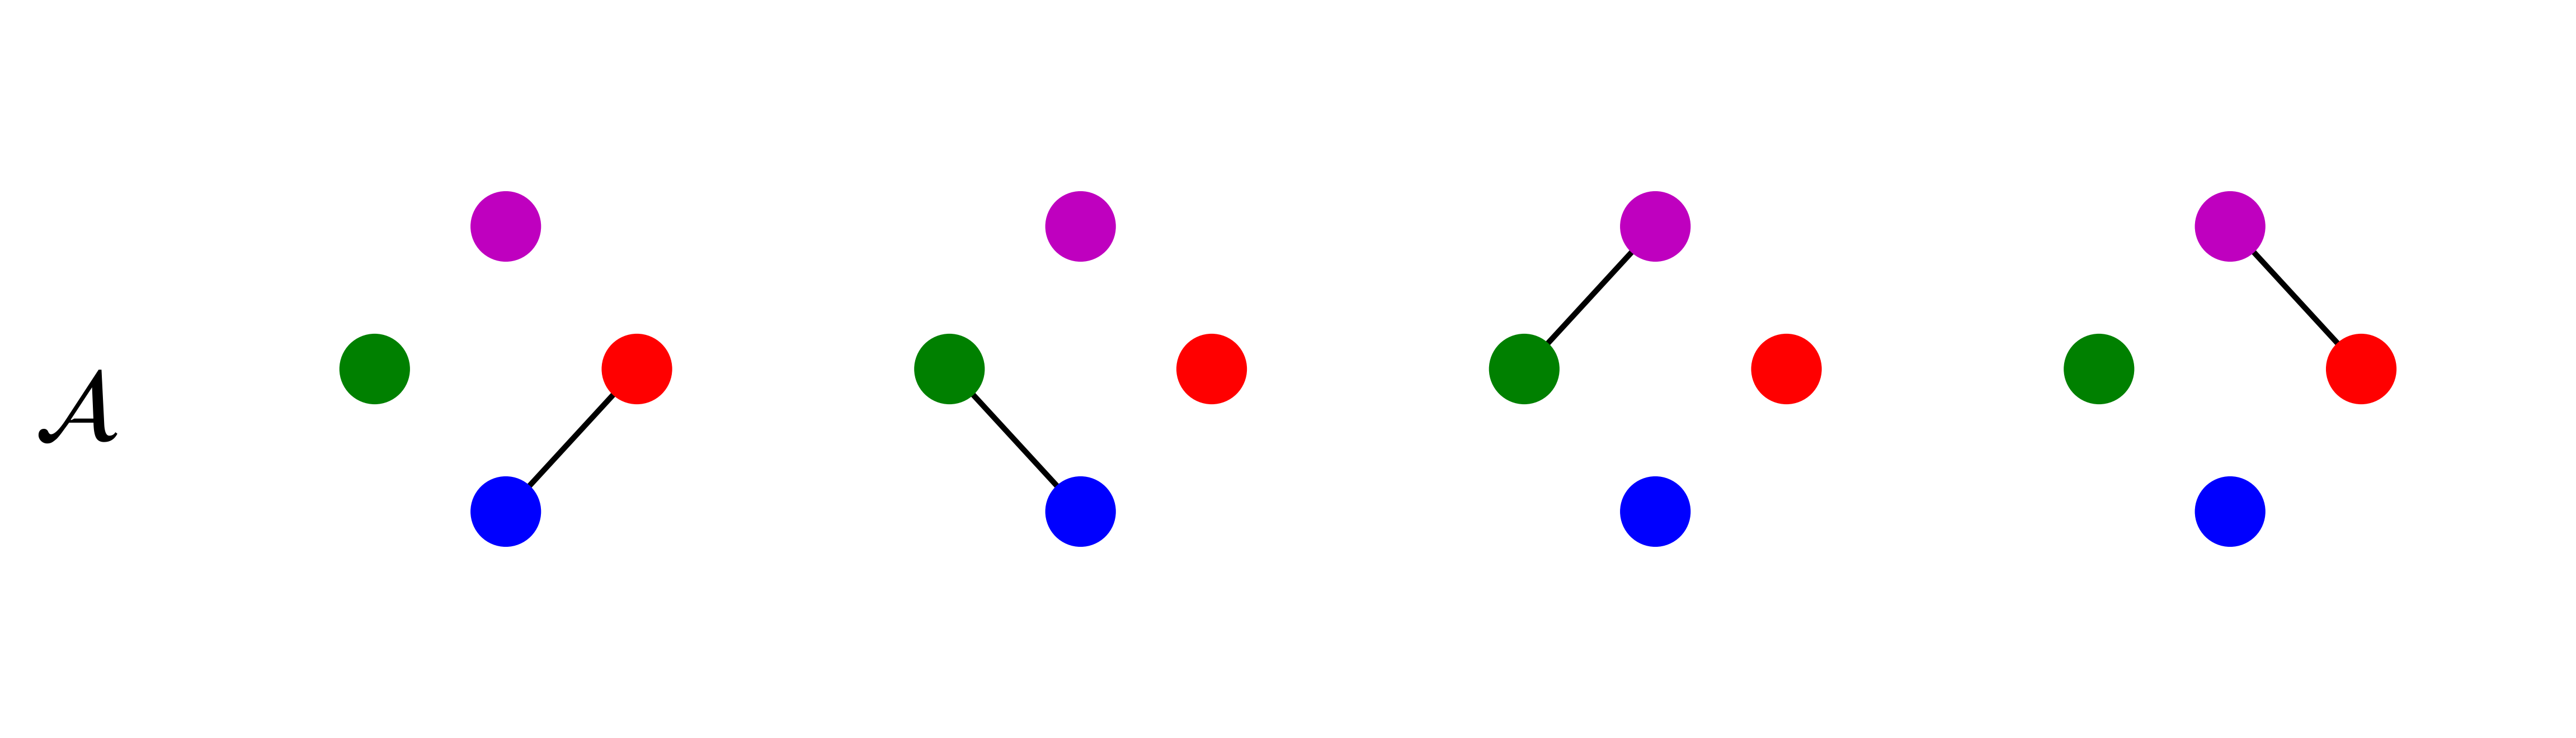
\includegraphics[width=0.48\textwidth]{fig/I0.png}
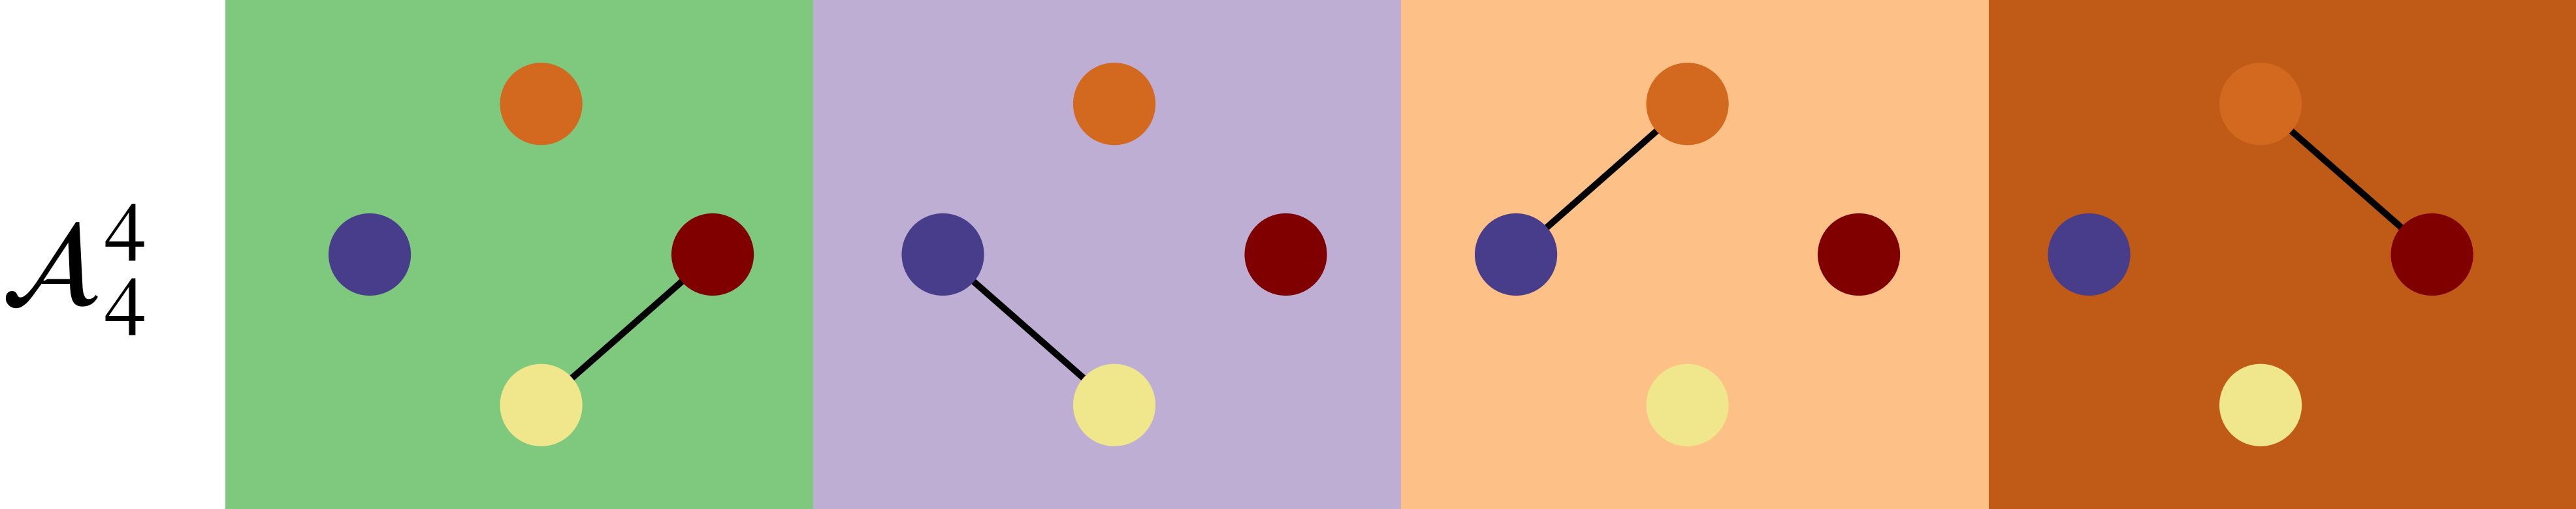
\includegraphics[width=0.48\textwidth]{fig/I4.png}
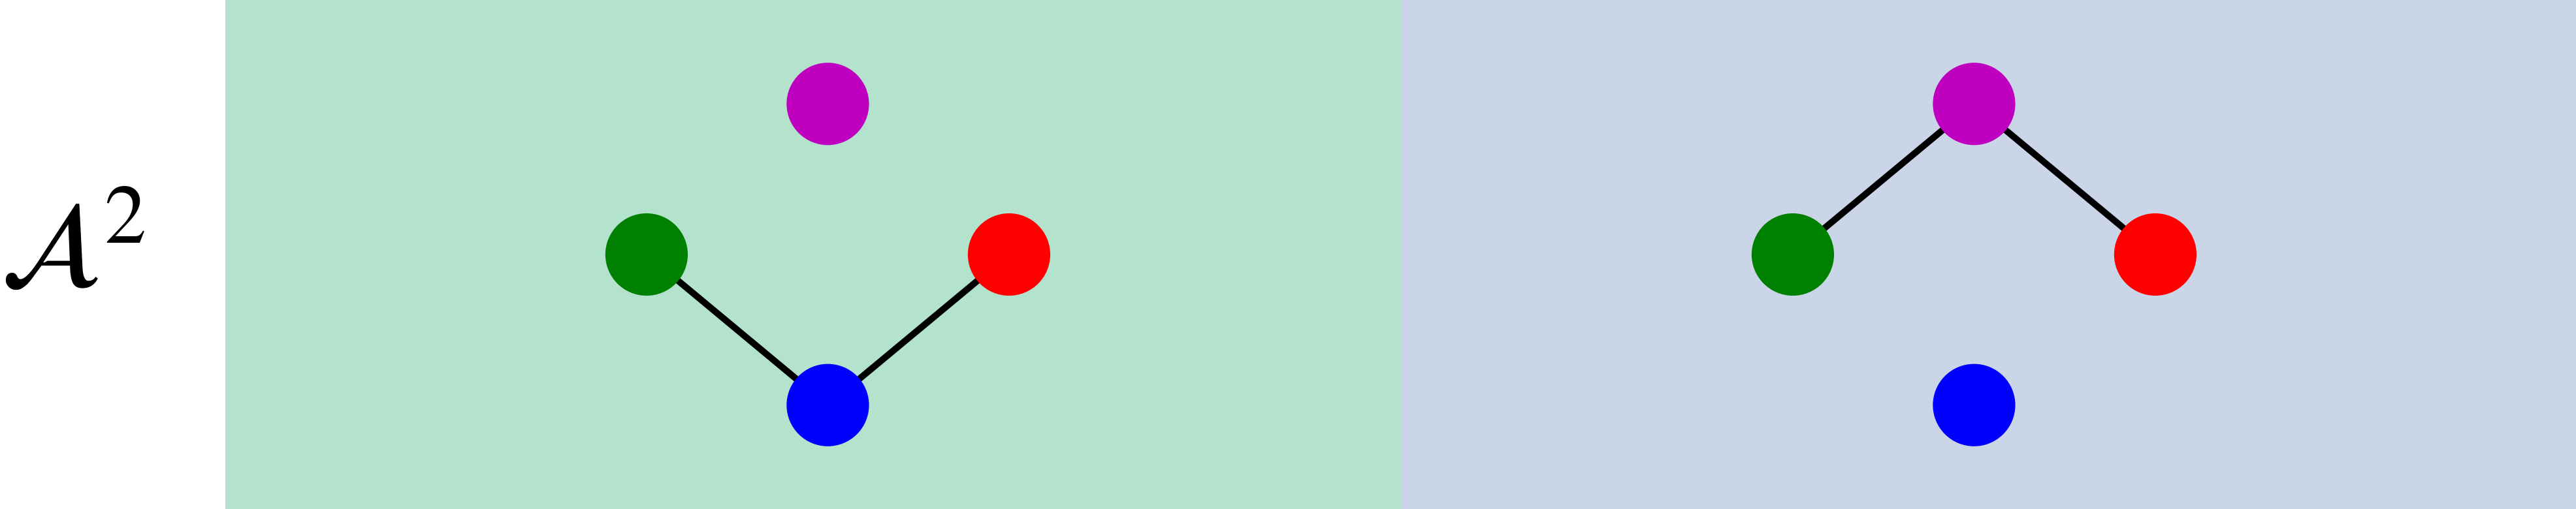
\includegraphics[width=0.48\textwidth]{fig/I2.png}
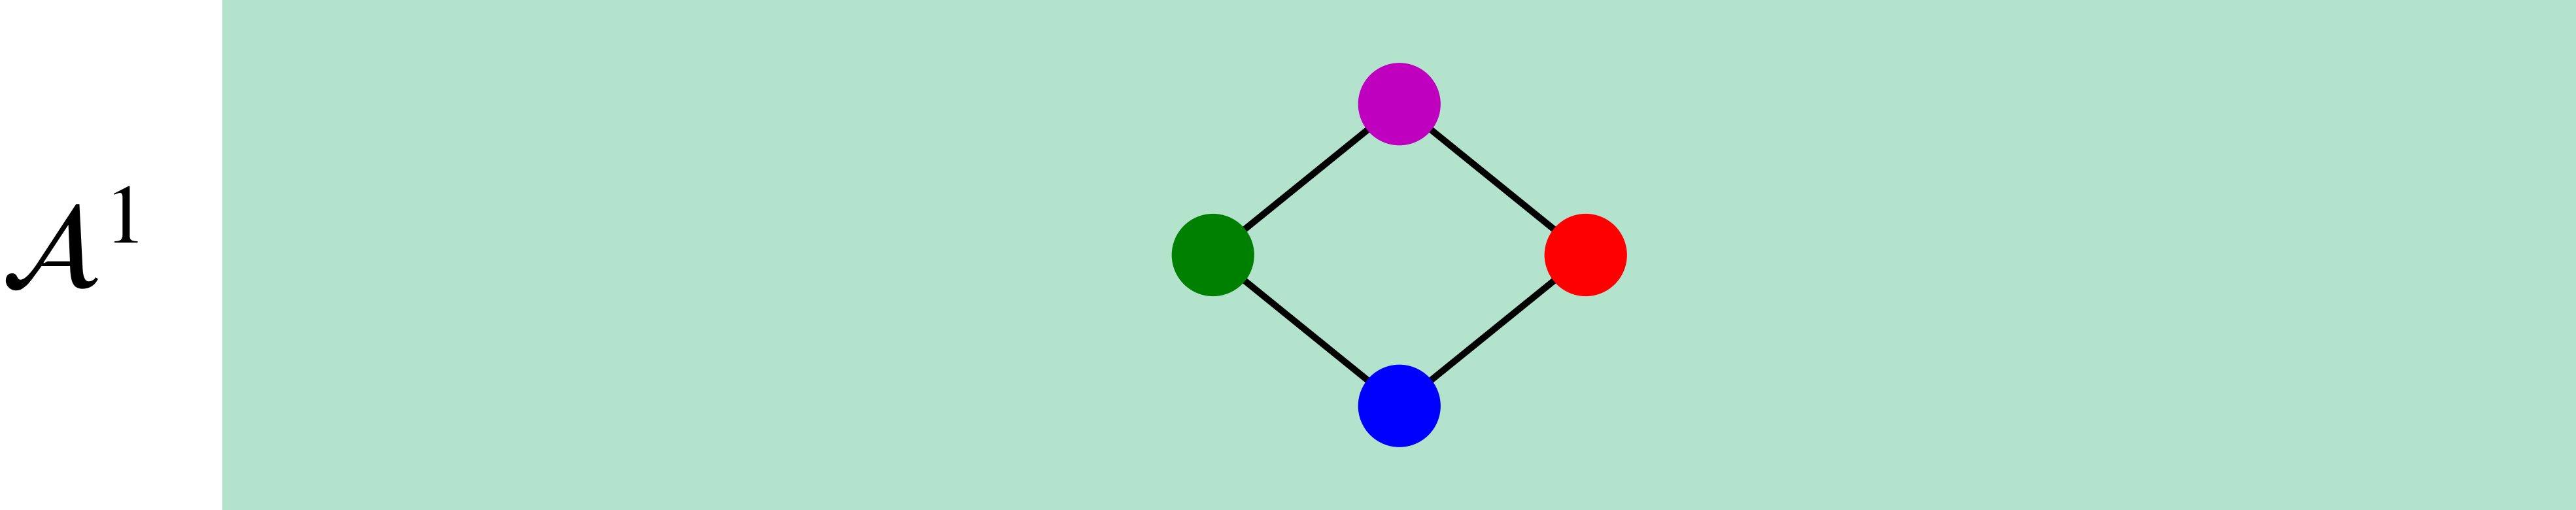
\includegraphics[width=0.48\textwidth]{fig/I1.png}
\caption{\label{fig:EXsub}Example of sub aggregated temporal networks $\mathcal{A}^I_T$ of an original temporal network $\mathcal{A}_4$ with four nodes and four snapshots for different aggregation intervals $I=\{1,2,4\}$.
}
\end{figure}

To calculate the accessibility $\mathcal{P}_{T}^{I}$ of the sub-aggregated temporal network $\mathcal{A}^I_T$, we allow for paths of same maximal length as in the accessibility $\mathcal{P}_{T}$ of %the original temporal network 
$\mathcal{A}_T$. Since each snapshot of $\mathcal{A}^I_T$ represents $T/I$ original snapshots, we allow for paths of maximal length $T/I$ in each snapshot of $\mathcal{A}^I_T$, i.e. treating each sub-aggregated adjacency matrix $\mathbb{A}_i$ as if it had occurred $T/I$ times, yielding
\begin{align} 
\mathcal{P}_{T}^{I} 
% = \hbox{sign}(\prod_{i=1}^{I} (\mathbf{1} + \mathbf{P}_{i,L})) 
= \hbox{sign}(\prod_{i=1}^{I} (\mathbf{1} + \mathbb{A}_i)^{T/I}) .
\label{eq:PAI}
\end{align}
% where $\mathbf{P}_{i,L}$ is the accessibility of $\mathbf{A}_i$ considering paths of maximal length $L$. 

Since sub aggregation only adds accessibility edges, the edge-set of $\mathcal{P}_T$ is a subset of the edge-set of $\mathcal{P}^I_T$, making  their union simplifying to the edge-set of $\mathcal{P}^I_T$, and their intersection to the edge-set of $\mathcal{P}_T$. Thus, the generalized causal fidelity for  $\mathcal{A}_T' = \mathcal{A}^I_T$  reduces to 
\begin{align}
\mathtt{C}(\mathcal{A}_T,\mathcal{A}^I_T) = \frac{|\mathcal{P}_T |}{|\mathcal{P}^I_T|}=\frac{\rho (\mathcal{P}_T )}{\rho (\mathcal{P}^I_T)},
\end{align}
where $\rho (\mathcal{P}_T)=N^{-2}\sum_{ij} (\mathcal{P}_T)_{ij}$ is the density of the accessibility matrix $\mathcal{P}_T$.
%The generalized causal fidelity measuring how well $\mathcal{A}^I_T$ represents $\mathcal{A}_T$ regarding its accessibility then reduces to $\mathtt{C}(\mathcal{A}_T,\mathcal{A}^I_T)%=J(\mathcal{P}_T, \mathcal{P}^I_T) =\frac{|\mathcal{P}_T \cap \mathcal{P}^I_T|}{|\mathcal{P}_T \cup \mathcal{P}^I_T|} =\frac{|\mathcal{P}_T |}{|\mathcal{P}^I_T|}$ which is equivalent to $\frac{\rho (\mathcal{P}_T )}{\rho (\mathcal{P}^I_T)}$ where $\rho (\cdot )$ is the density of the accessibility matrix. 

%%%%%%%% Limit Cases
The original temporal network $\mathcal{A}_T$ and the fully aggregated static network $\mathbf{A}$ are limit-cases of $\mathcal{A}^I_T$. 
In the limiting case of no aggregation ($I=T$), we have $\mathcal{A}^T_T = \mathcal{A}_T$ and $\mathbb{A}_i = \mathbf{A}_i$ for all $i$.
%For the former, by considering $T$ intervals ($I=T$) each snapshot gets its own interval and nothing is aggregated.
The generalized causal fidelity then compares the original temporal network $\mathcal{A}_T$ with itself, resulting in $\mathtt{C}(\mathcal{A}_T,\mathcal{A}^T_T)=\mathtt{C}(\mathcal{A}_T,\mathcal{A}_T)=1$. 
Contrary, when only one interval ($I=1$) is considered the whole temporal network $\mathcal{A}_T$ is aggregated. In this case the accessibility $\mathcal{P}^1_T$ of $\mathcal{A}^1_T$  coincides with the accessibility $\mathbf{P}_T$ of the fully aggregated static network $\mathbf{A}$, 
resulting in the causal fidelity $\mathtt{C}(\mathcal{A}_T,\mathcal{A}_T^1)= \frac{\rho (\mathcal{P}_T )}{\rho (\mathbf{P}_T)}$ introduced in  \cite{lentz2013unfolding}. 

Throughout the paper we limit ourselves to the analysis of the generalized causal fidelity of sub aggregated temporal networks.  For the sake of simplicity, in the following we set $\mathtt{C}^I_T \equiv \mathtt{C}(\mathcal{A}_T,\mathcal{A}^I_T)$.




%%%%%%%
\section{\label{sec:results}Results}


\subsection{\label{sec:ANAresults}
Emerging accessibility in uncorrelated temporal networks}

% In this section, we provide an analytical estimation of the range of temporal network lengths for which aggregation leads to maximal information loss in random temporal networks. To do this, we leverage on the 
% connection between path saturation in the aggregated network and the temporal network length.

Let us consider random temporal network defined as a set of $T$ snapshots each with a probability for edge occurrence fixed to $q$ and $N$ nodes.
If the snapshots are independent, and the process is memory-less, we can establish a connection between the aggregated static network $\mathbf{A}$, or $\mathcal{A}^I_T$ with $I=1$, and the probability for temporal edge occurrence $q$.
In particular, each edge in $\mathbf{A}$ is present if it is present in at least one of the $T$ snapshots. Therefore an edge in the aggregated static network is present with probability $p=1-(1-q)^T$, which is the complementary probability that an edge never occurs in $T$ snapshots. Thus, the aggregated static network can be seen as a static random network with edge-probability $p=\braket{k}/N$, where $\braket{k}=N^{-1}\sum_{ij}\mathbf{A}_{ij}$ is the average degree of the fully aggregated network.
% For $I=1$, the generalized causal fidelity $\mathtt{C}^1_T$ measures wrong accessibility caused by wrongly implied paths in the aggregated static network $\mathbf{A}$ that are not present in the temporal network $\mathcal{A}_T$.
% Eq. \eqref{eq:pagg} shows that the edge-probability $p$ of the aggregated network increases as the temporal network length $T$ increases, given a fixed $q$. 
By inverting the previous relation we get  
\begin{eqnarray}
T(p,q)=\frac{\ln(1-p)}{\ln(1-q)}
\label{eq:Tagg},
\end{eqnarray}
which expresses the temporal network length as function of the edge creation probabilities of the single snapshots $q$ and of the fully aggregated network $p$.
Thus, given $q$, there is a \emph{critical length} of a temporal network  $T_c={\ln(1-p_c)}/{\ln(1-q)}$ for which a giant connected component emerges in the aggregated network. 
By inserting the critical value $p_c=1/N$ \cite{ERevolution} in eq. \eqref{eq:Tagg}, we get
\begin{eqnarray}
T_c=\frac{\ln(1-{1}/{N})}{\ln(1-q)}
\label{eq:TC1},
\end{eqnarray}
which provides a lower bound for the emergence of a giant connected component in the underlying aggregated network.

Analogously, we can find an upper bound corresponding to the saturation of a giant connected component in the fully aggregated temporal network. 
A static random graph can be expected to almost surely be fully connected for $p\ge p_f = {\ln(N)}/{N}$  as the giant component probability saturates \cite{ERevolution}. If the aggregated network is fully connected and  $T>N$, the accessibility graph is fully connected and full accessibility is reached, i.e. $\mathbf{P}_T$ is the matrix of all ones. The corresponding temporal network length $T_f$ where the edge-probability in the aggregated network satisfies $p = p_f$ is then
\begin{eqnarray}
T_f=\frac{\ln(1-{\ln(N)}/{N})}{\ln(1-q)} 
\label{eq:TC2}.
\end{eqnarray}

Since a path between two nodes can only exist if they belong to the same connected component, the accessibility in the aggregated network $\mathbf{A}$  directly relates to connectedness. 
Within the giant connected component of size $G$ each node can reach all other nodes and it contributes $G^2$ accessibility edges to the accessibility graph.
Fig.~\ref{fig:ERgiantsq} shows the comparison between the relative size of largest connected component squared $G^2$ and the density $\rho_T^1 \equiv \rho(\mathcal{P}_T^1)$ of the fully-aggregated accessibility graph defined by eq. \eqref{eq:PAI} with $T_c$ (blue vertical line) and $T_f$ (red vertical line). The comparison shows that for $T>T_c$, the increase of the density of the accessibility graph is mainly driven by the largest connected component. 
In the next sections, we validate numerically this model for synthetic and empirical temporal networks and identify the temporal network length interval $T_c<T<T_f$ for which the causal fidelity displays a global minimum corresponding to maximal information loss due to aggregation.
To avoid sample specific effects, we average our results from the considered baseline temporal network $\mathcal{A}_T$ over time intervals of the same length. 
This means that for temporal network lengths $(T)$ we sample from the baseline temporal network intervals of the form  $[\mathbf{A}_t,\mathbf{A}_{t+T-1}]$ at different values of $t$. 
Thus, the results have to be understood as averages and single temporal networks might deviate substantially.



\begin{figure}[]
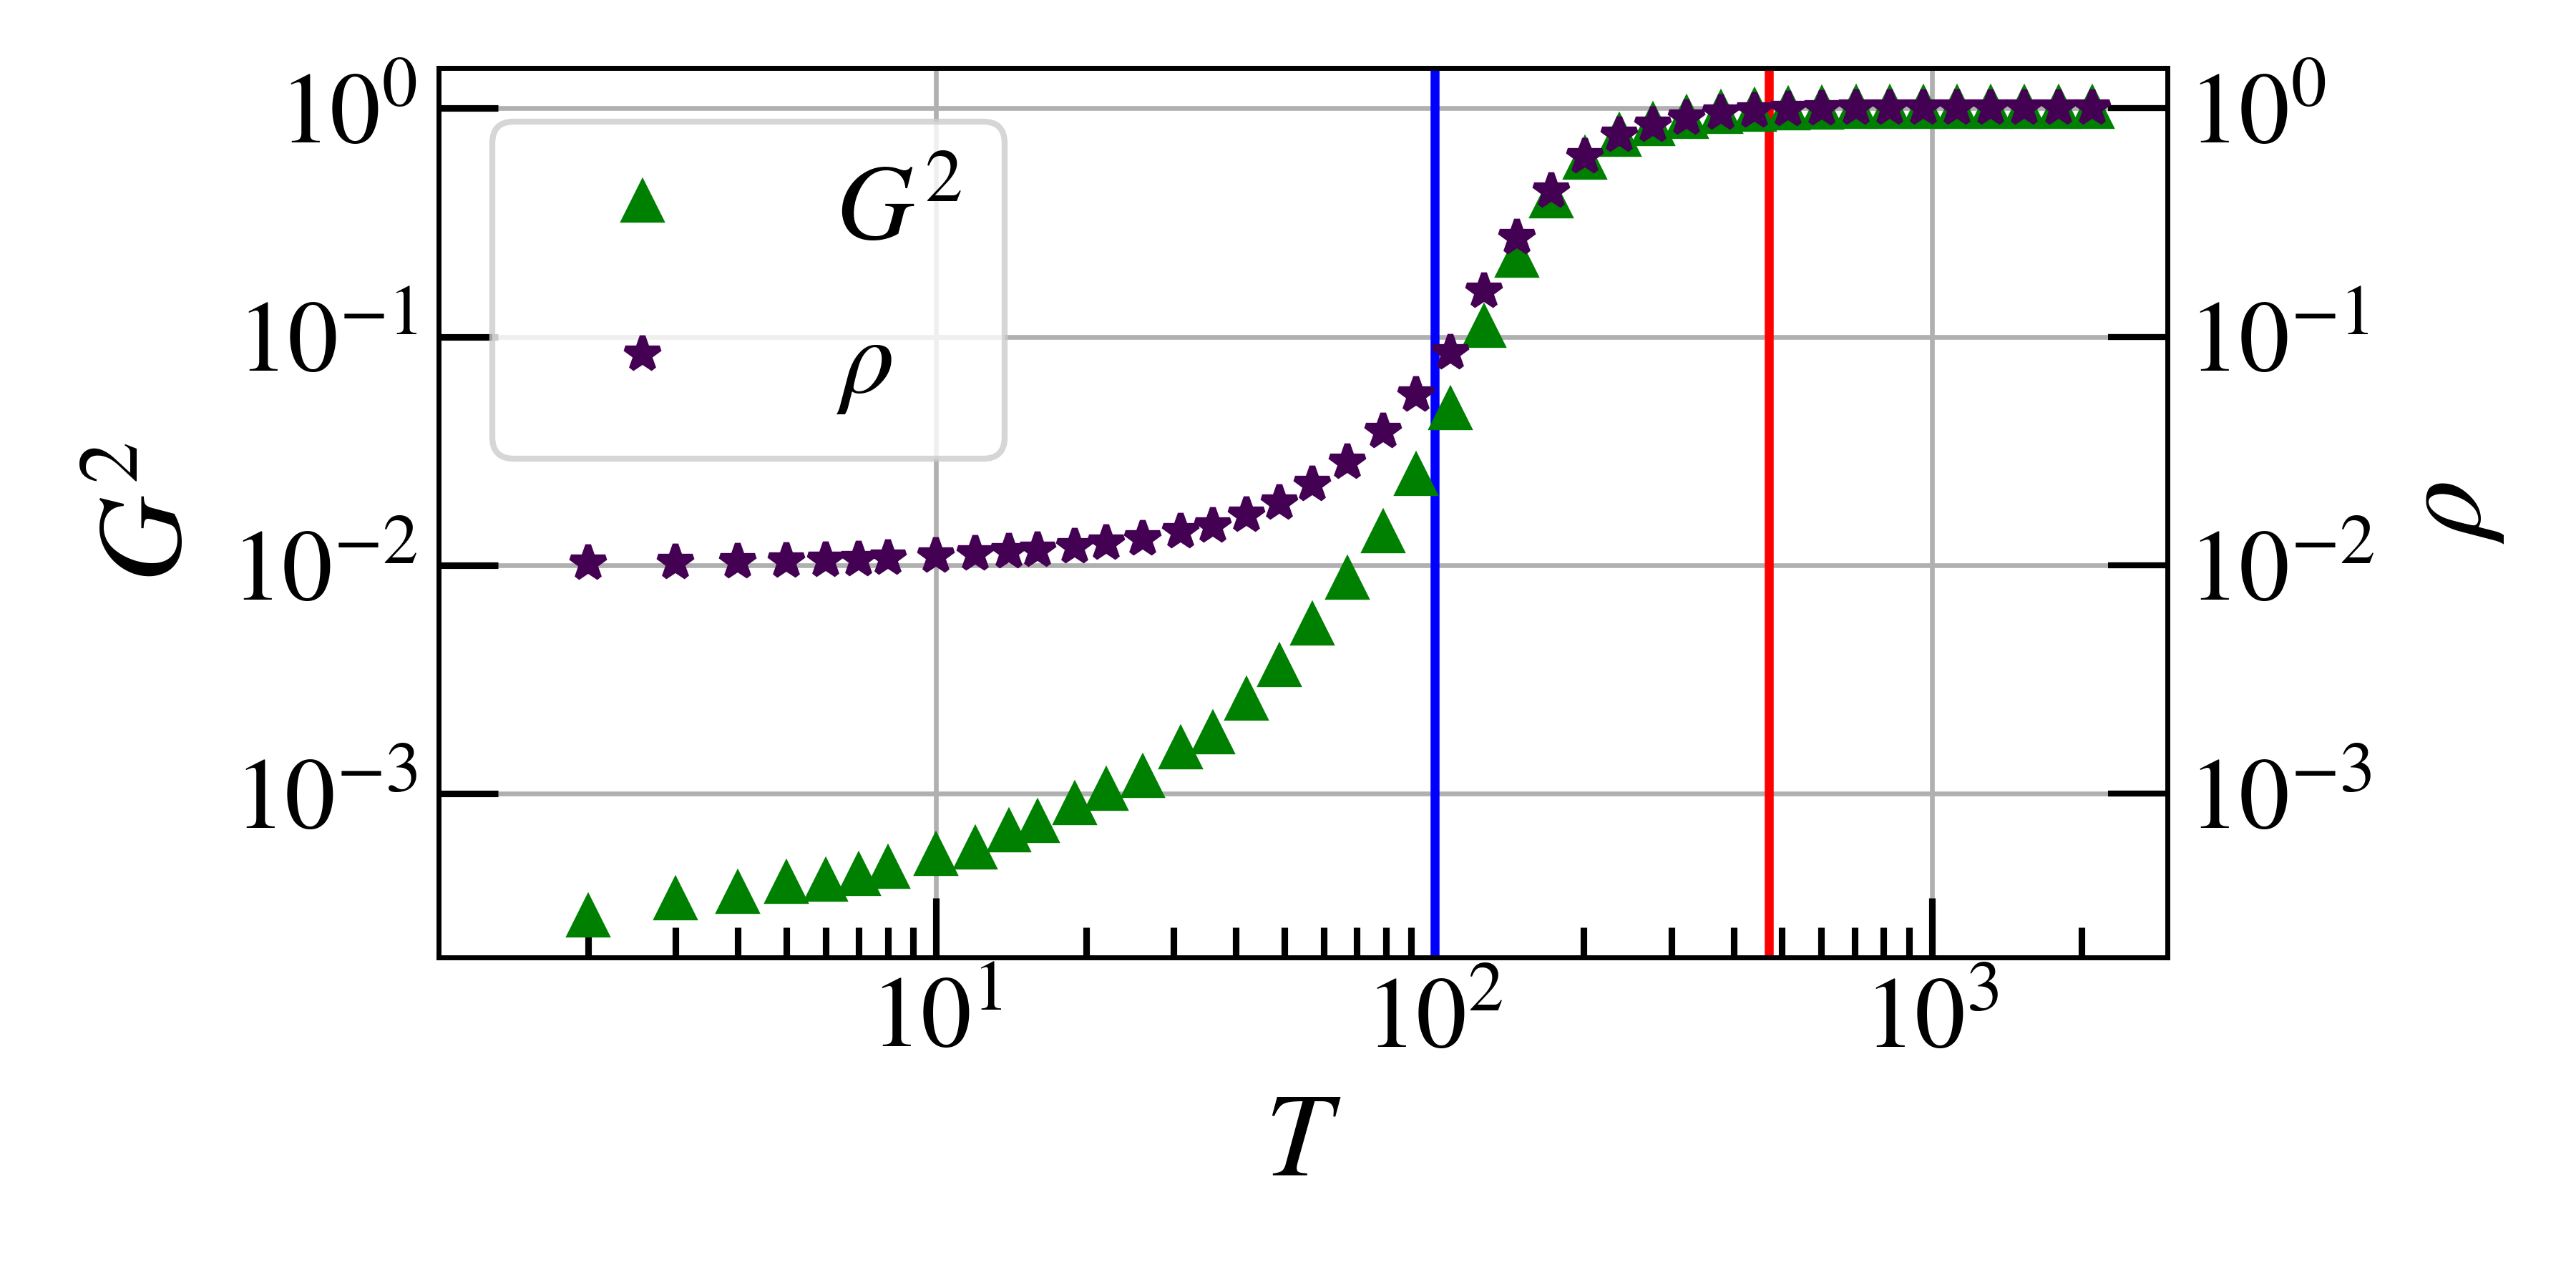
\includegraphics[width=0.48\textwidth]{fig/ER_G_ana2_log.png}
\caption{\label{fig:ERgiantsq} Relative size of the largest connected component squared $G^2$ (stars) and density of the accessibility matrix (triangles) for the full aggregate ($I=1$), for artificially generated random temporal networks with $N=100$ nodes and  edge probability $q= 0.0001$. The vertical blue line marks the critical value $T_c$ defined by eq. \eqref{eq:TC1} corresponding to the emergence of the giant component in the fully aggregated network, while the red vertical line marks the temporal network length $T_f$ defined by eq. \eqref{eq:TC2} where the probability for giant components saturates to the maximum value. 
}
\end{figure}






\subsection{\label{sec:ERresults} Poisson random networks}


\begin{figure}[]
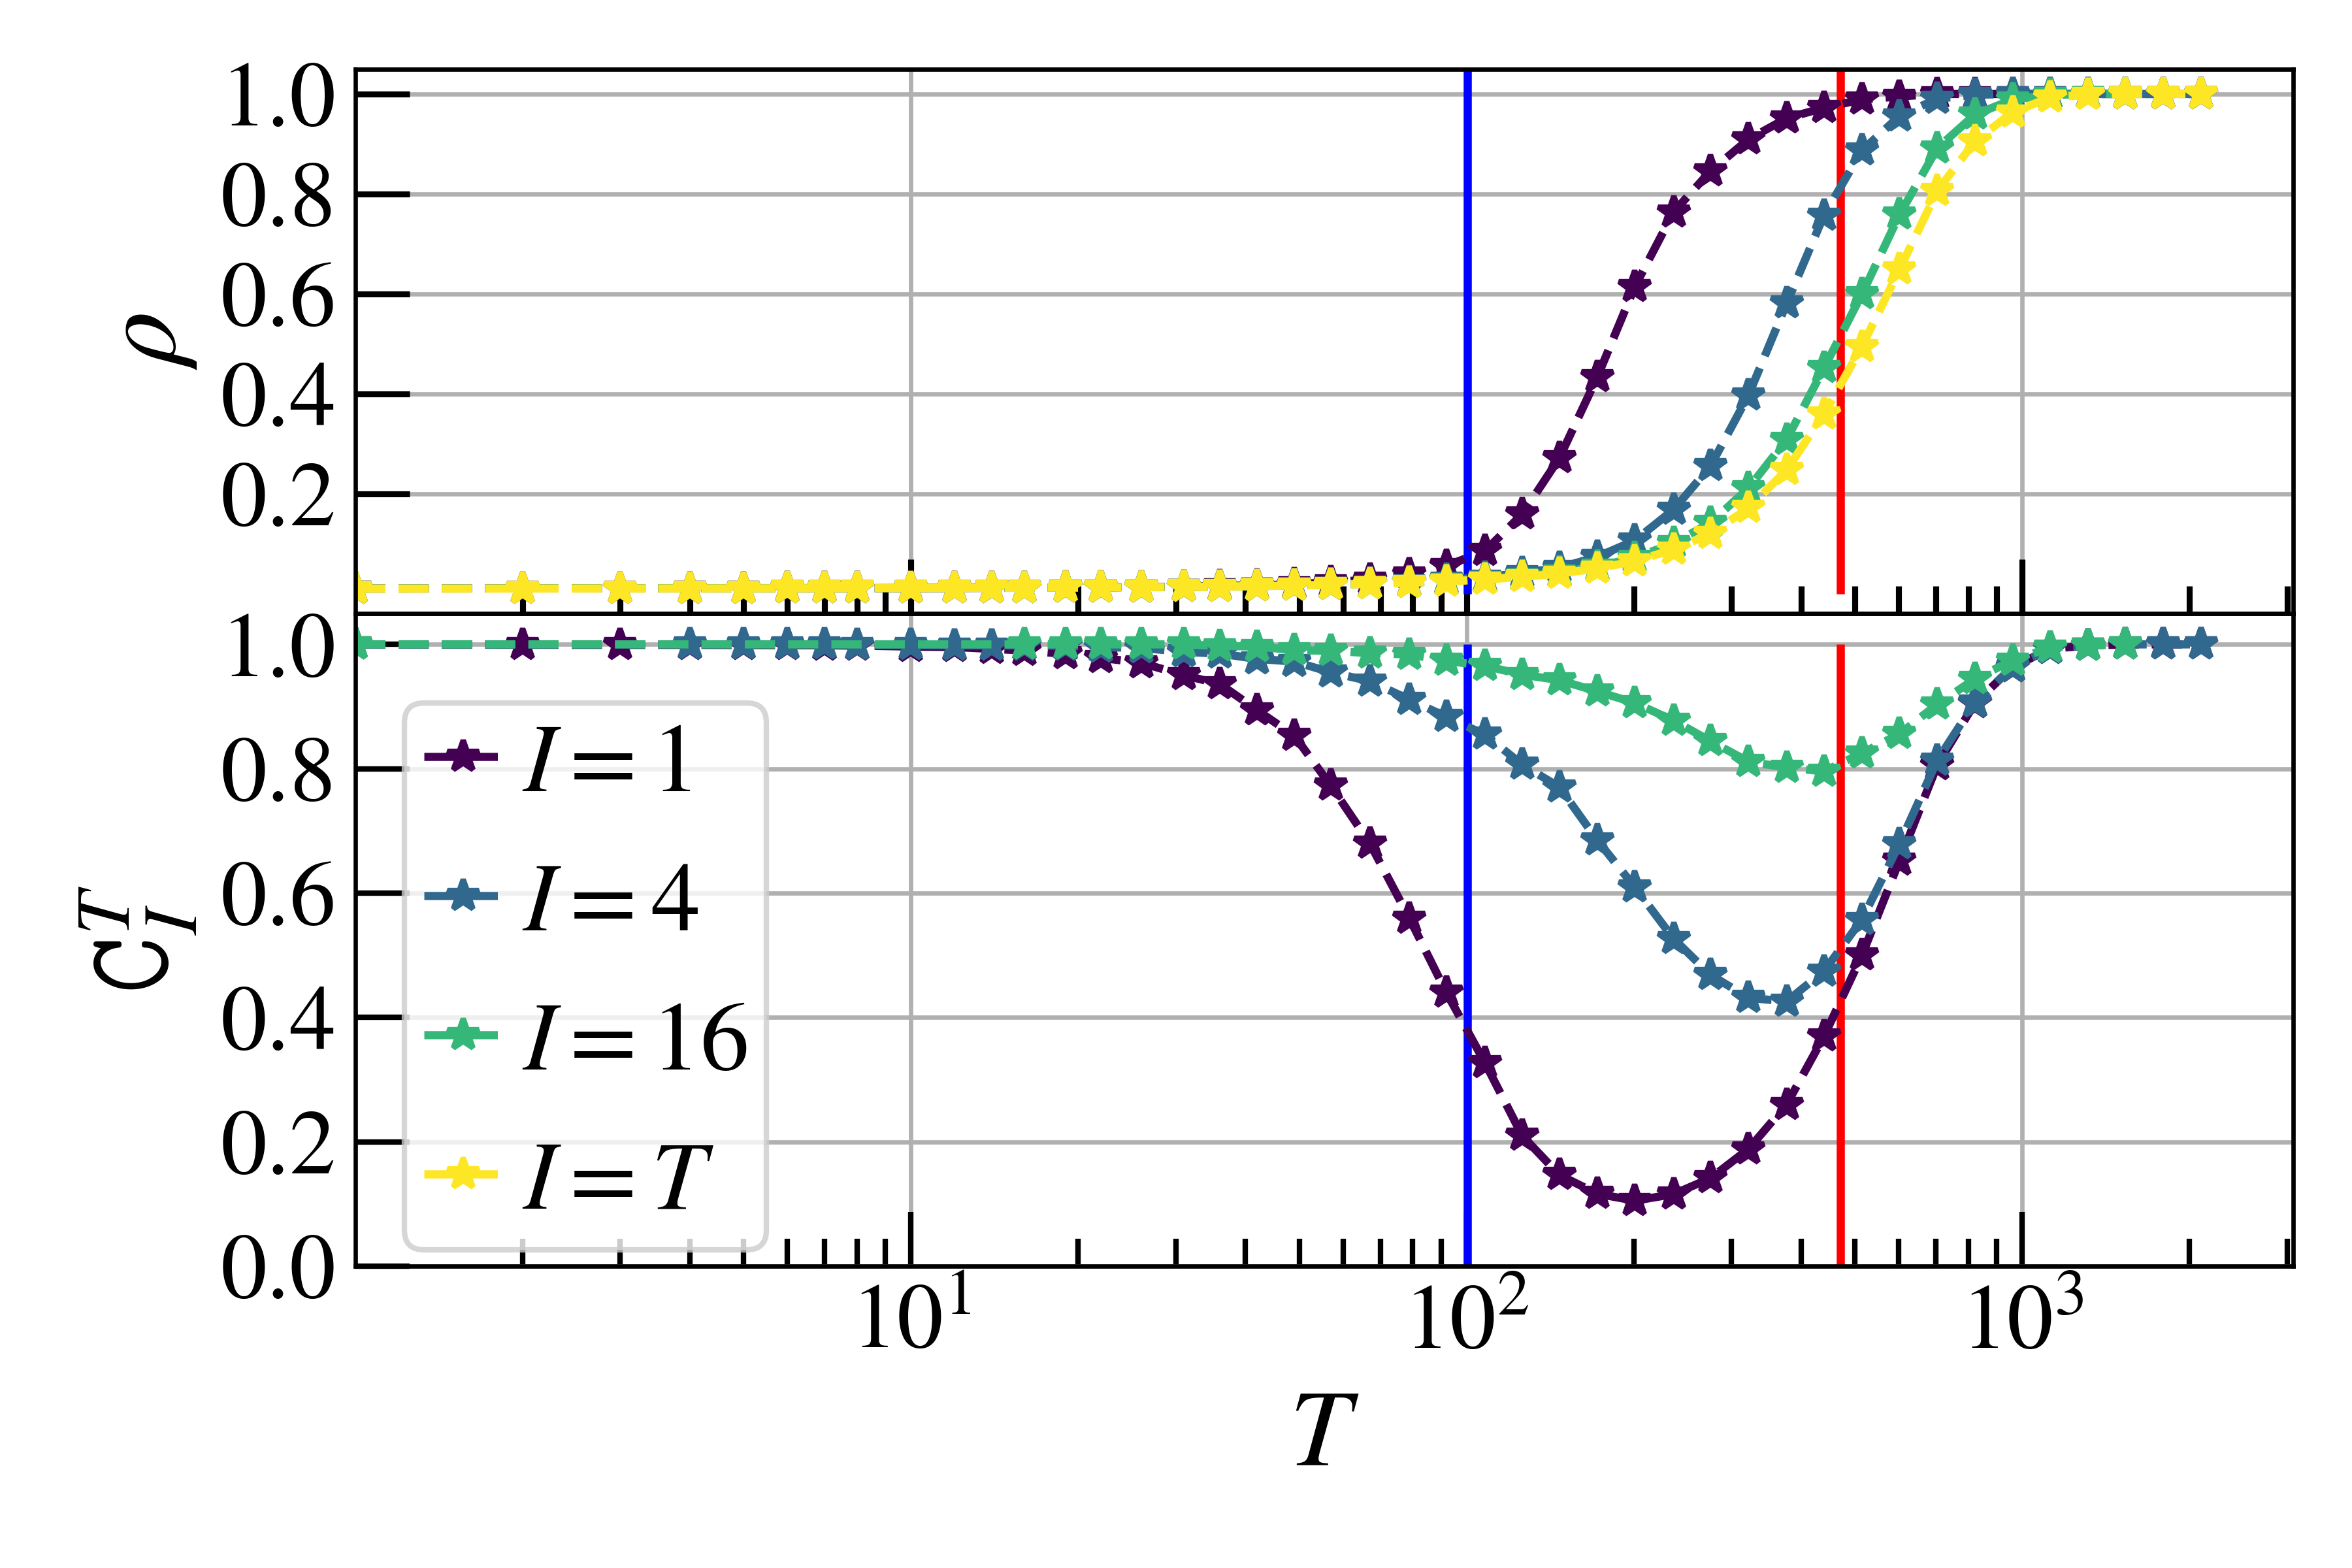
\includegraphics[width=0.48\textwidth]{fig/ER_cr.png}
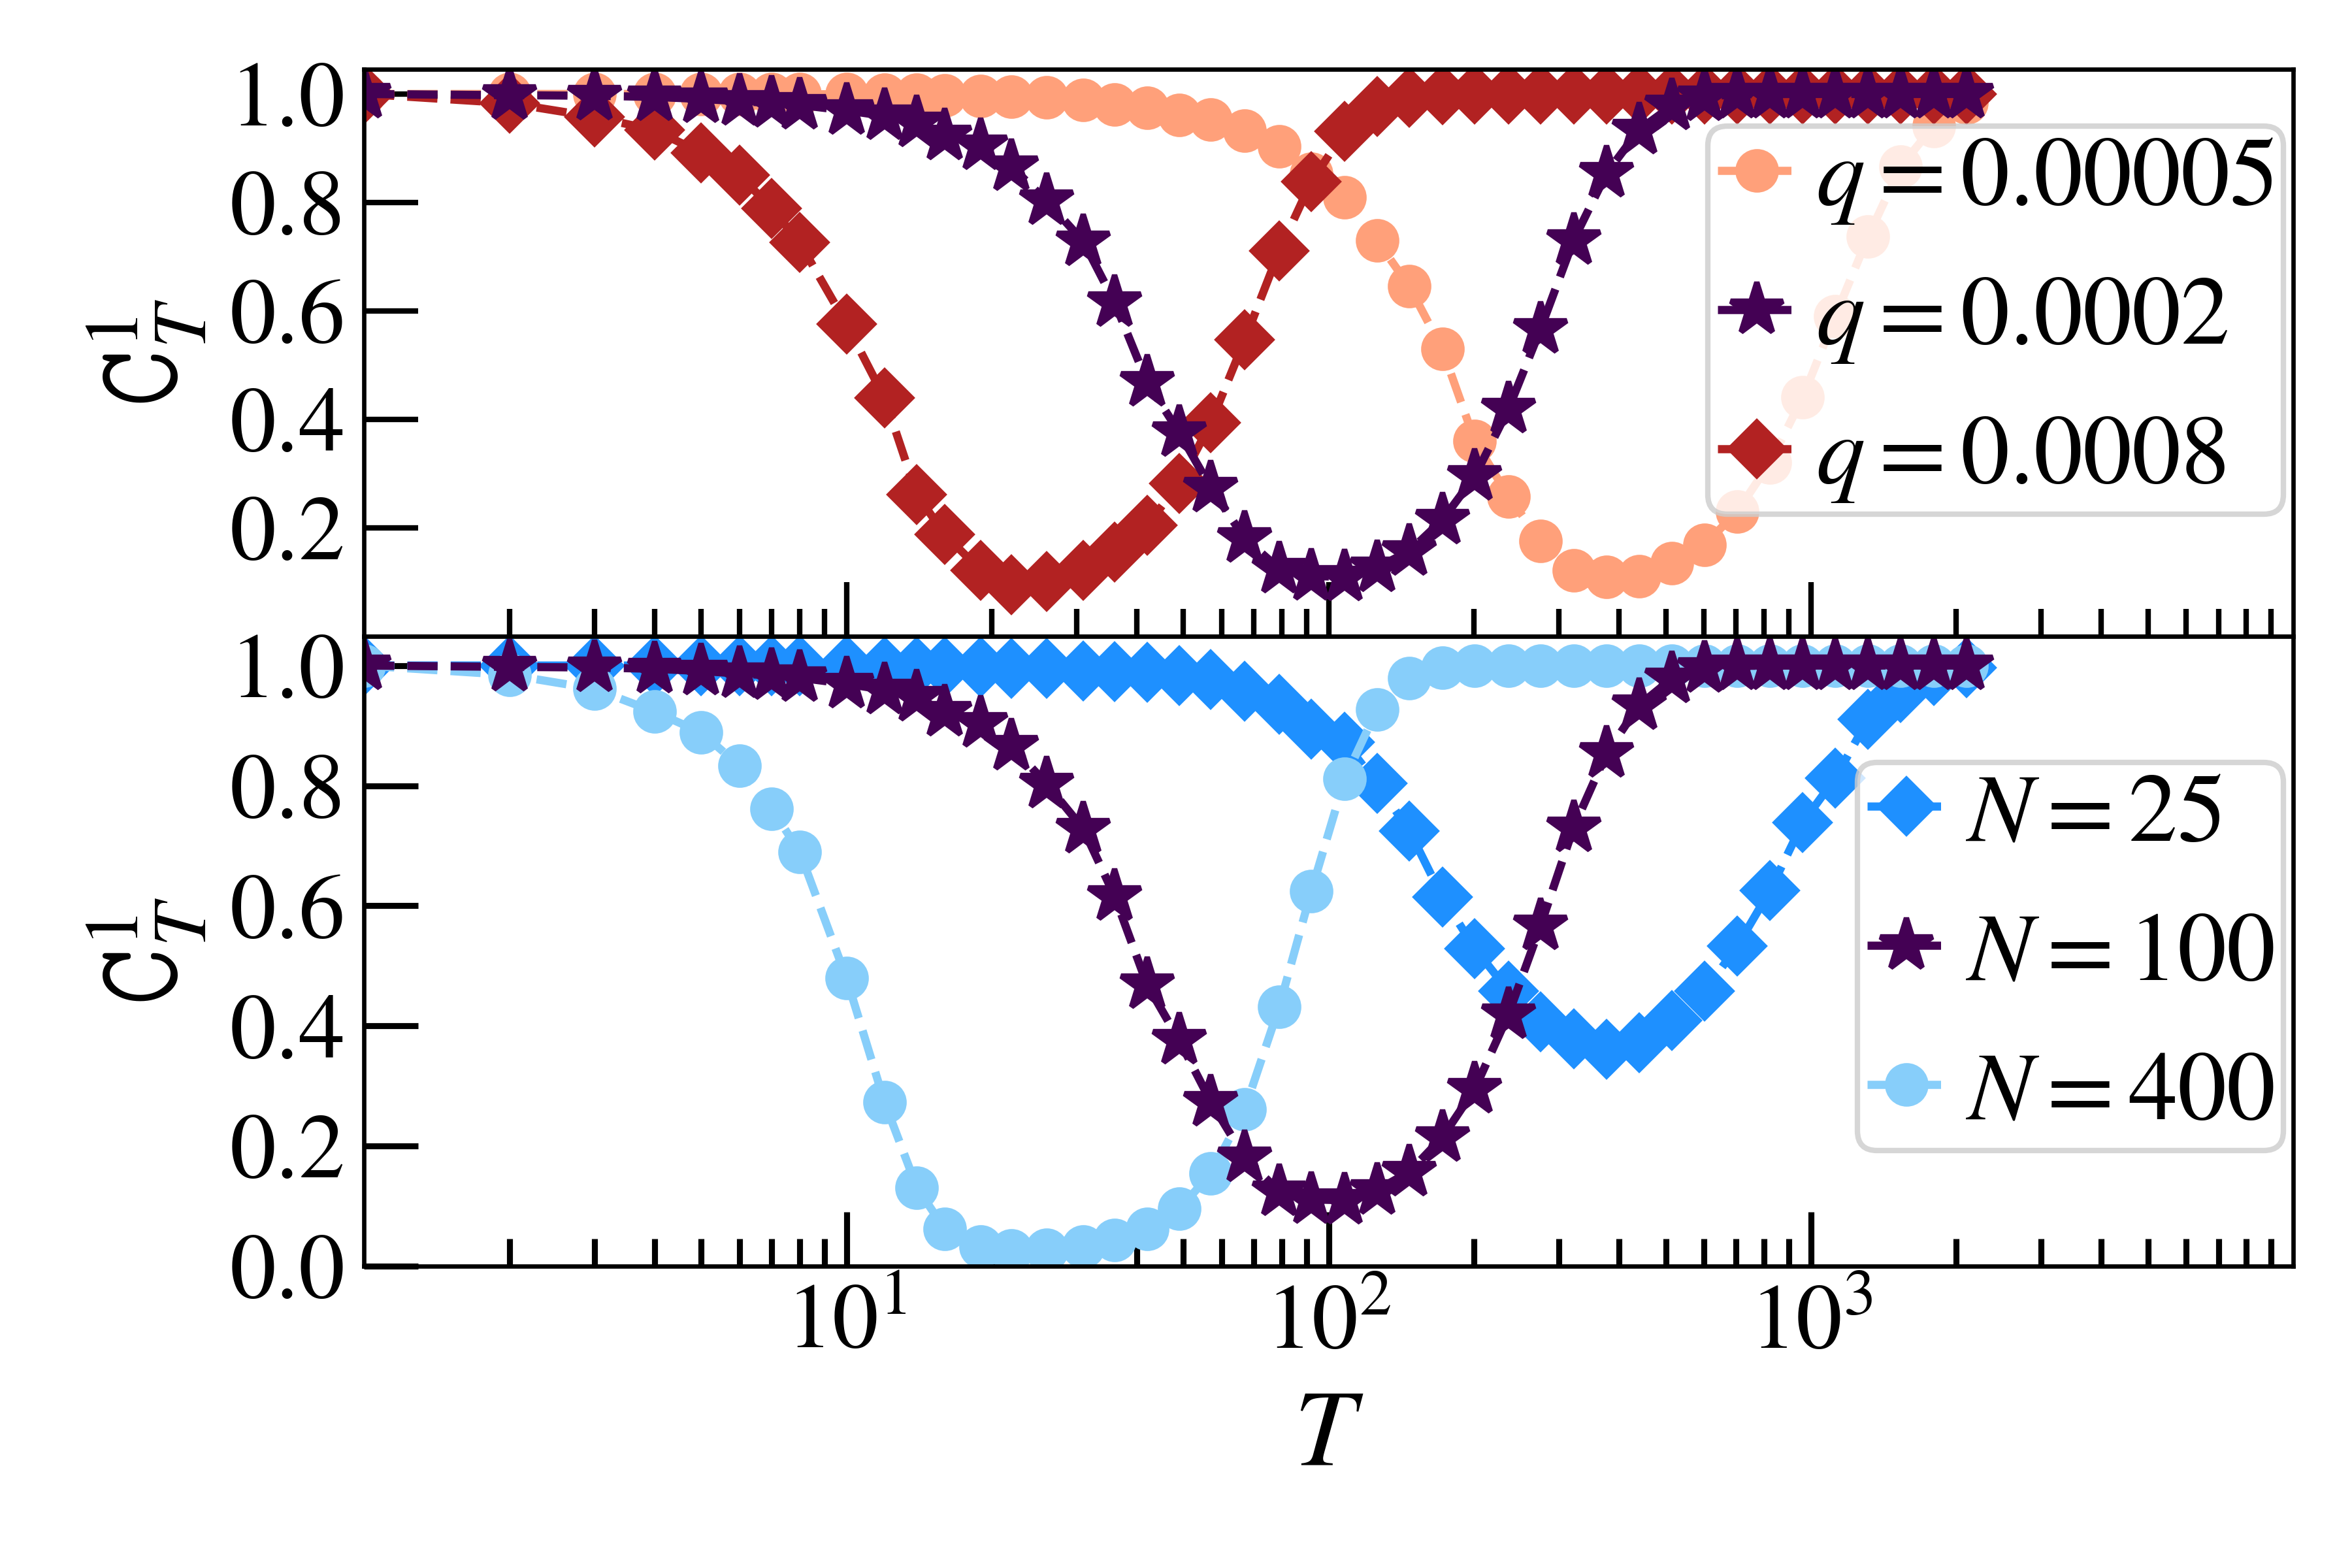
\includegraphics[width = 0.48\textwidth]{fig/ER_Nq.png}
\caption{\label{fig:ERcf} Upper panel: Results for artificially generated random temporal networks with $N=100$ nodes and  edge probability $q= 0.0002$ as a function of the temporal network length $T$ for different number of aggregation intervals $I$.
Comparison between density of the accessibility matrix $\rho(\mathcal{P}^I_T)$ and 
generalized causal fidelity $\mathtt{C}^I_T$. 
Different colors refer to different sub-aggregation interval numbers $I$.
The blue vertical line marks the critical value $T_c$ for the emergence of a giant component in the fully aggregated network, while the red vertical marks the value  $T_f$ for which the fully aggregated network saturates to a fully connected graph, see eq. \eqref{eq:TC1} and eq. \eqref{eq:TC2}. Lower panel: Generalized causal fidelity for different values of the snapshot edge probability $q$ with $N=100$ and different number of nodes $N$ with $q=0.0002$. 
}
\end{figure}

Let us first consider random temporal networks where each snapshot is an Erd\"os-R\'enyi (ER) graph. We study how the generalized causal fidelity $\mathtt{C}^I_T$ for sub-aggregated temporal networks  $\mathcal{A}^I_T$ depends on the length $T$ and on the aggregation interval number $I$.

In the upper panel of Fig.~\ref{fig:ERcf} we show the density $\rho_T^I$ of the accessibility $\mathcal{P}^I_T$, and the generalized causal fidelity $\mathtt{C}^I_T$, as function of the temporal network length $T$, for ER temporal networks with $N=100$ nodes and snapshot edge probability $q=0.0002$.
Different colors represent different aggregation interval numbers  $I$ and the vertical lines mark the analytical estimations given by $T_c$ and $T_f$. 
% From above we know that $\mathtt{C}^I_T= \frac{\rho (\mathcal{P}_T )}{\rho (\mathcal{P}^I_T)}$, that is the ratio between the density of the accessibility of the baseline temporal network%$\rho (\mathcal{P}_T)$
% , corresponding to $I=T$, and the density  of the accessibility of the sub aggregated temporal network%$\rho (\mathcal{P}^I_T)$ 
% . 
Different $I$ curves of causal fidelity corresponds to the ratio between the density at $I=T$ and the density at the same value of $I$. 
For $I=1$, i.e. when we aggregate the whole temporal network, we find that at low values of $T$ the sub aggregated temporal network perfectly represents the underlying baseline network, and no information is lost.  As $T$ increases, $\mathtt{C}^1_T$ decreases, indicating that the sub aggregated temporal network is a worse representation for the underlying baseline network.
Interestingly, we find a global minimum where the baseline network is represented worst. $\mathtt{C}^1_T$ then increases until a perfect representation is reached. $\rho_T^I$ shows that the density of the accessibility of the aggregated temporal network saturates faster then for the non-aggregated network. This shows the origin of the information loss: the aggregation causes more nodes to be connected by paths which may not be present in the underlying baseline network. Only once full saturation is reached for the underlying baseline network, implying that there exists a temporal path between all nodes, the generalized causal fidelity reaches its maximum value $\mathtt{C}^I_T=1$. The interval $T_c<T<T_f$, where the minimum of $\mathtt{C}^1_T$ is found, quantifies the range in temporal network lengths for which the aggregated static network is a poor representation of the original temporal network. 
For different values of $I$ the minimum of $\mathtt{C}^I_T$ appears for higher values of $T$ and it is less pronounced as expected, since more aggregation intervals correspond to less overall aggregation. The density behavior shows that the saturation of the accessibility matrix appears closer to the one in the baseline network compared to $I=1$.  

In the lower panel of Fig.~\ref{fig:ERcf} we plot the curves for $\mathtt{C}^1_T$ of the full aggregate for different values of the snapshot edge probability $q$, fixing the number of nodes to $N= 100$, and varying the number of nodes $N$, with fixed $q= 0.0002$.
Interestingly, the minima of the casual fidelity only shift in time when we vary the snapshot edge probability $q$, but their value remain constant $\mathtt{C}^1_T\approx 0.1$.
Contrary, there is a clear dependence on the size of the network, with lower values corresponding to a shift toward higher values of $T$ for the location of the minima but to a lower drop in causal fidelity. For $q= 0.0002$, it is sufficient to have $N=400$ to practically have vanishing casual fidelity between the original temporal network and the fully aggregated one, resulting in complete loss of information. 


This analytical point of view gives  us the insight that the generalized causal fidelity is mainly driven by connected components, and the emergence of such components is directly related to the activity of the nodes.
The emergence of connected components happens earlier in aggregated networks than in non-aggregated. This shift leads to low generalized causal fidelity until the underlying network catches up with the connectedness of the aggregated one. 
%%%%%%%
% Finally, it turns out that we can estimate the location of the minimum $T_m$ of the generalized causal fidelity by $T_m=\exp((\ln T_c+\ln T_f)/2) = \sqrt{T_c T_f}$. \fla{we need an alternative argument to justify this or to provide in the appendix the results of the log-normal fits on synthetic and real networks} Using the expressions of the previous estimators $T_c$ and $T_f$ for the emergence of the giant component at $p_c$ and for the saturation probability $p_G=\ln(N)/N$, we find 
% \begin{eqnarray}
% T_m= \frac{\sqrt{\ln(1-{\ln(N)}/{N}){\ln(1-{1}/{N}})}}{\ln(1-q)}
% \label{eq:TC3}.
% \end{eqnarray}
% \fla{thermodynamic limit expansion leads to $T_m\approx \sqrt{\ln N}/(N\ln(1-q))$}


%%%%%%% generalization to SBM
% \subsubsection{\label{sec:ERresults}Random temporal network with two blocks}

\begin{figure}[]
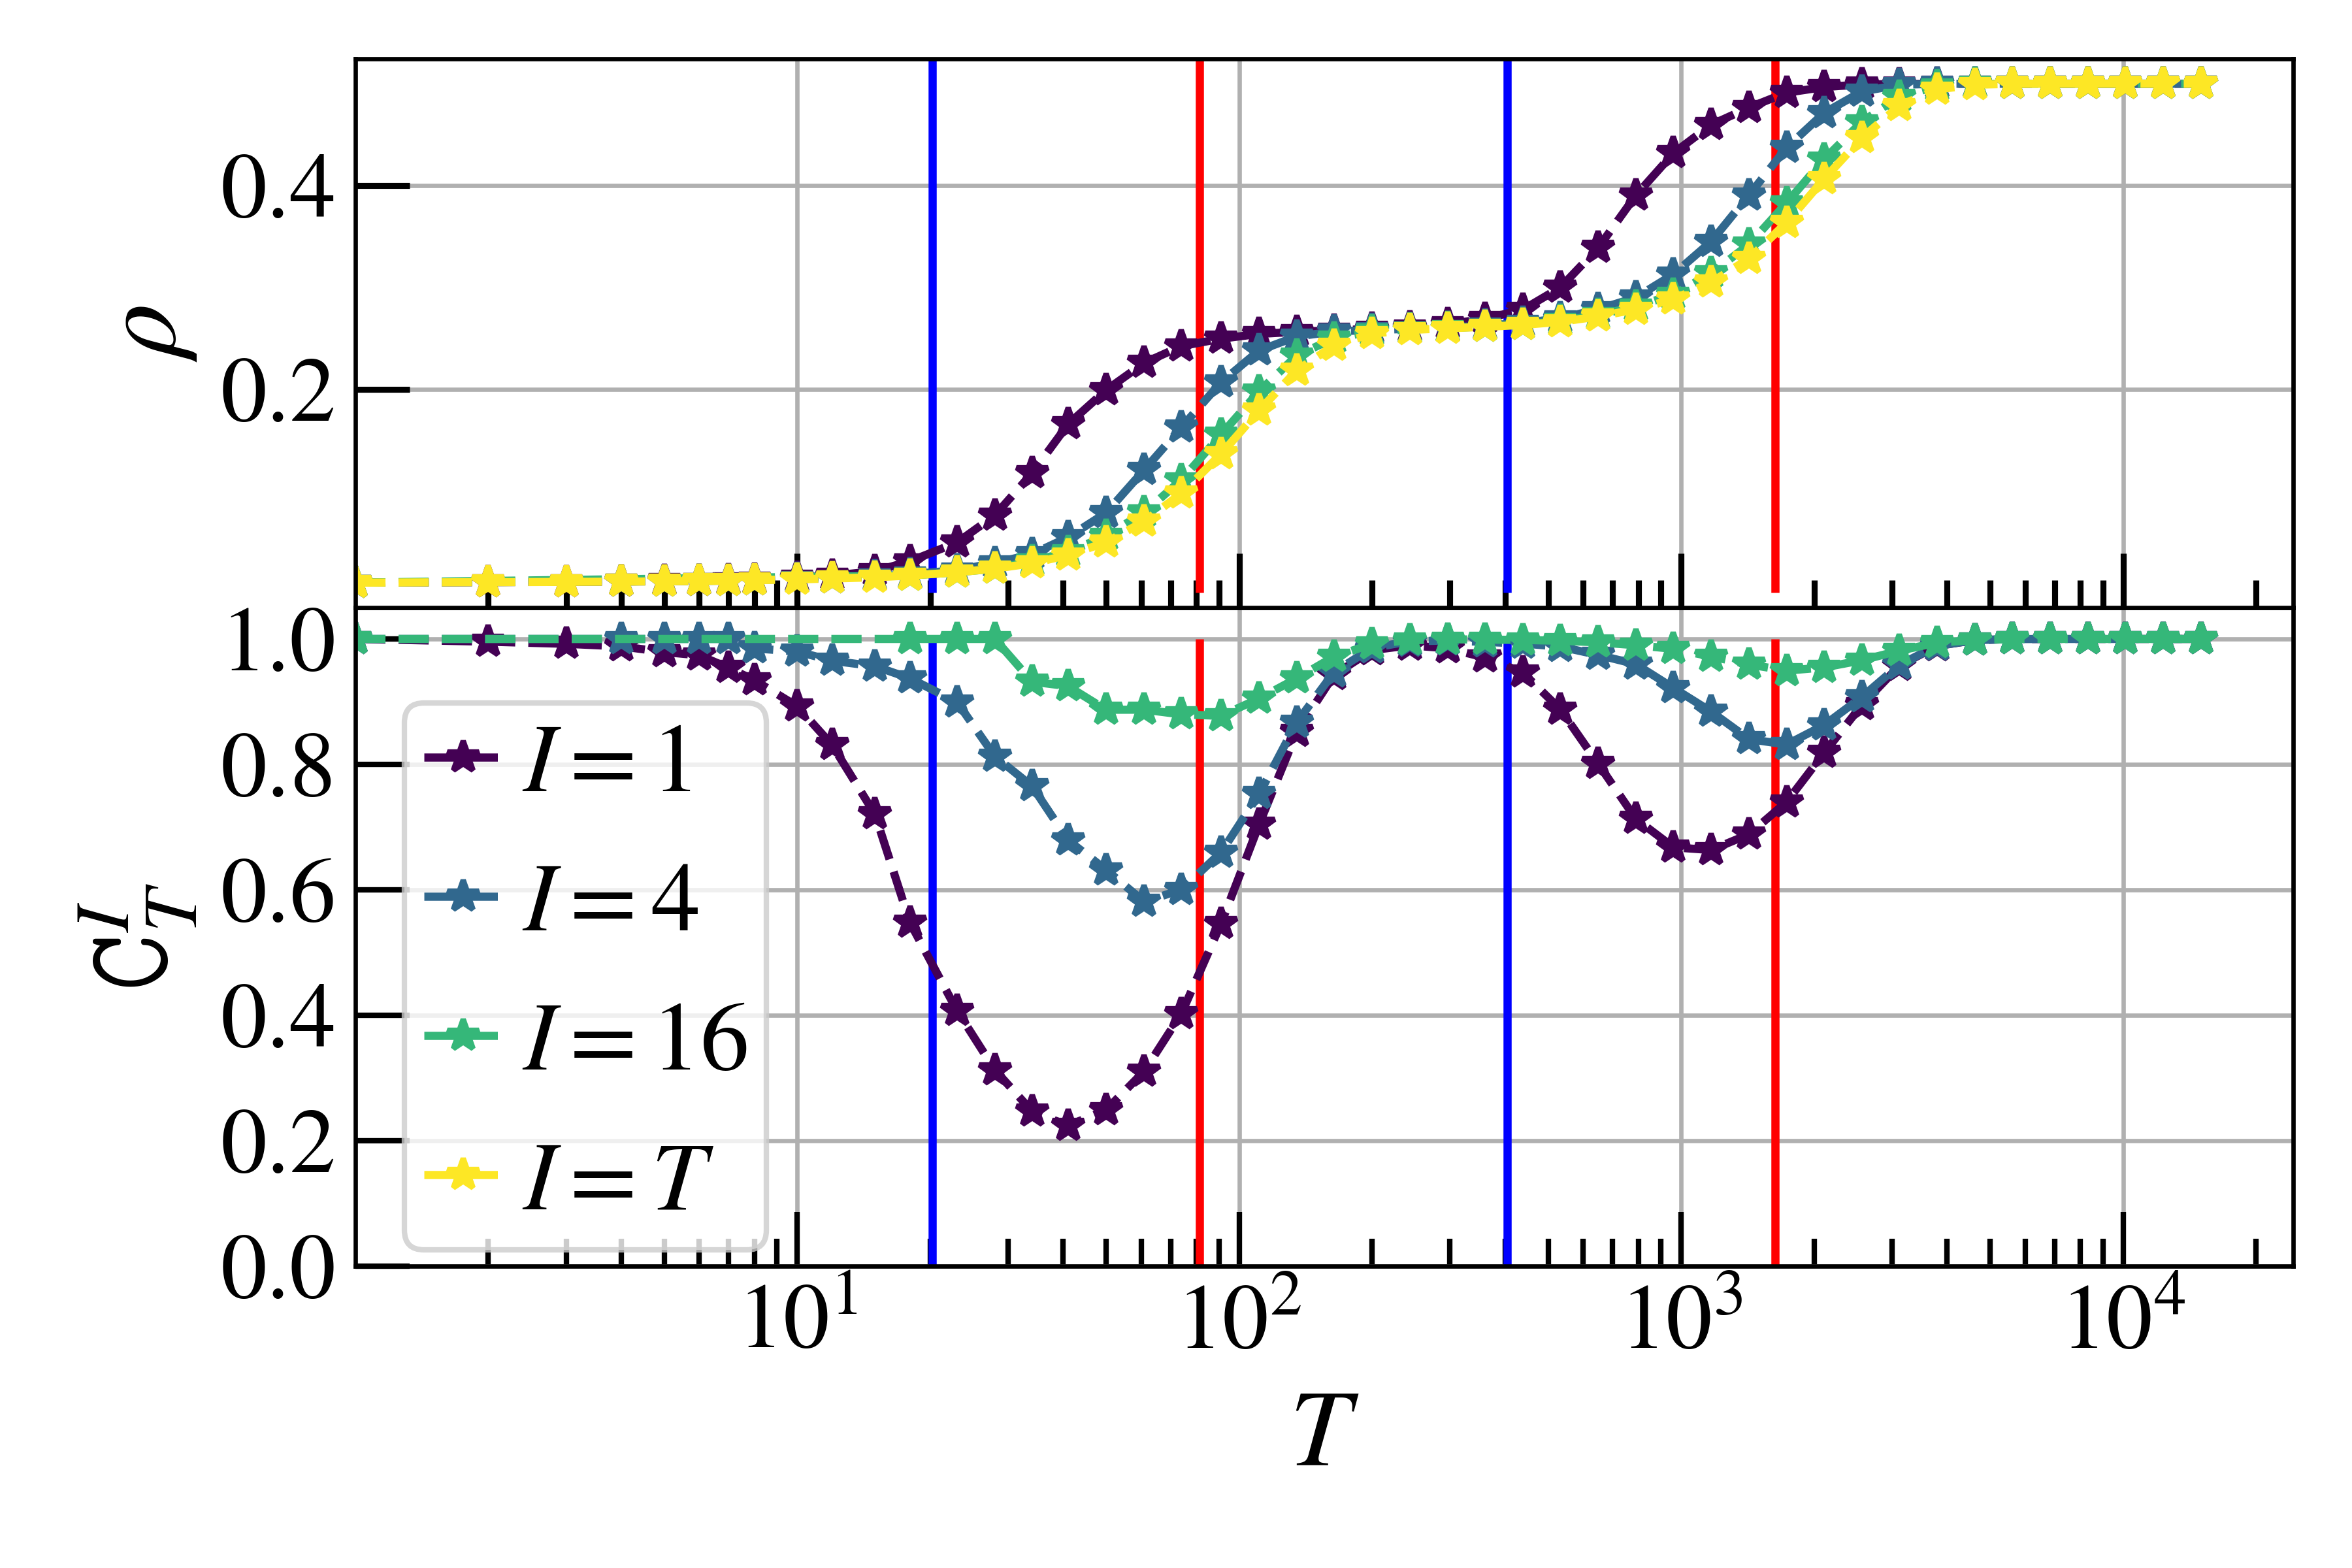
\includegraphics[width=0.48\textwidth]{fig/SBM_cr.png}
% 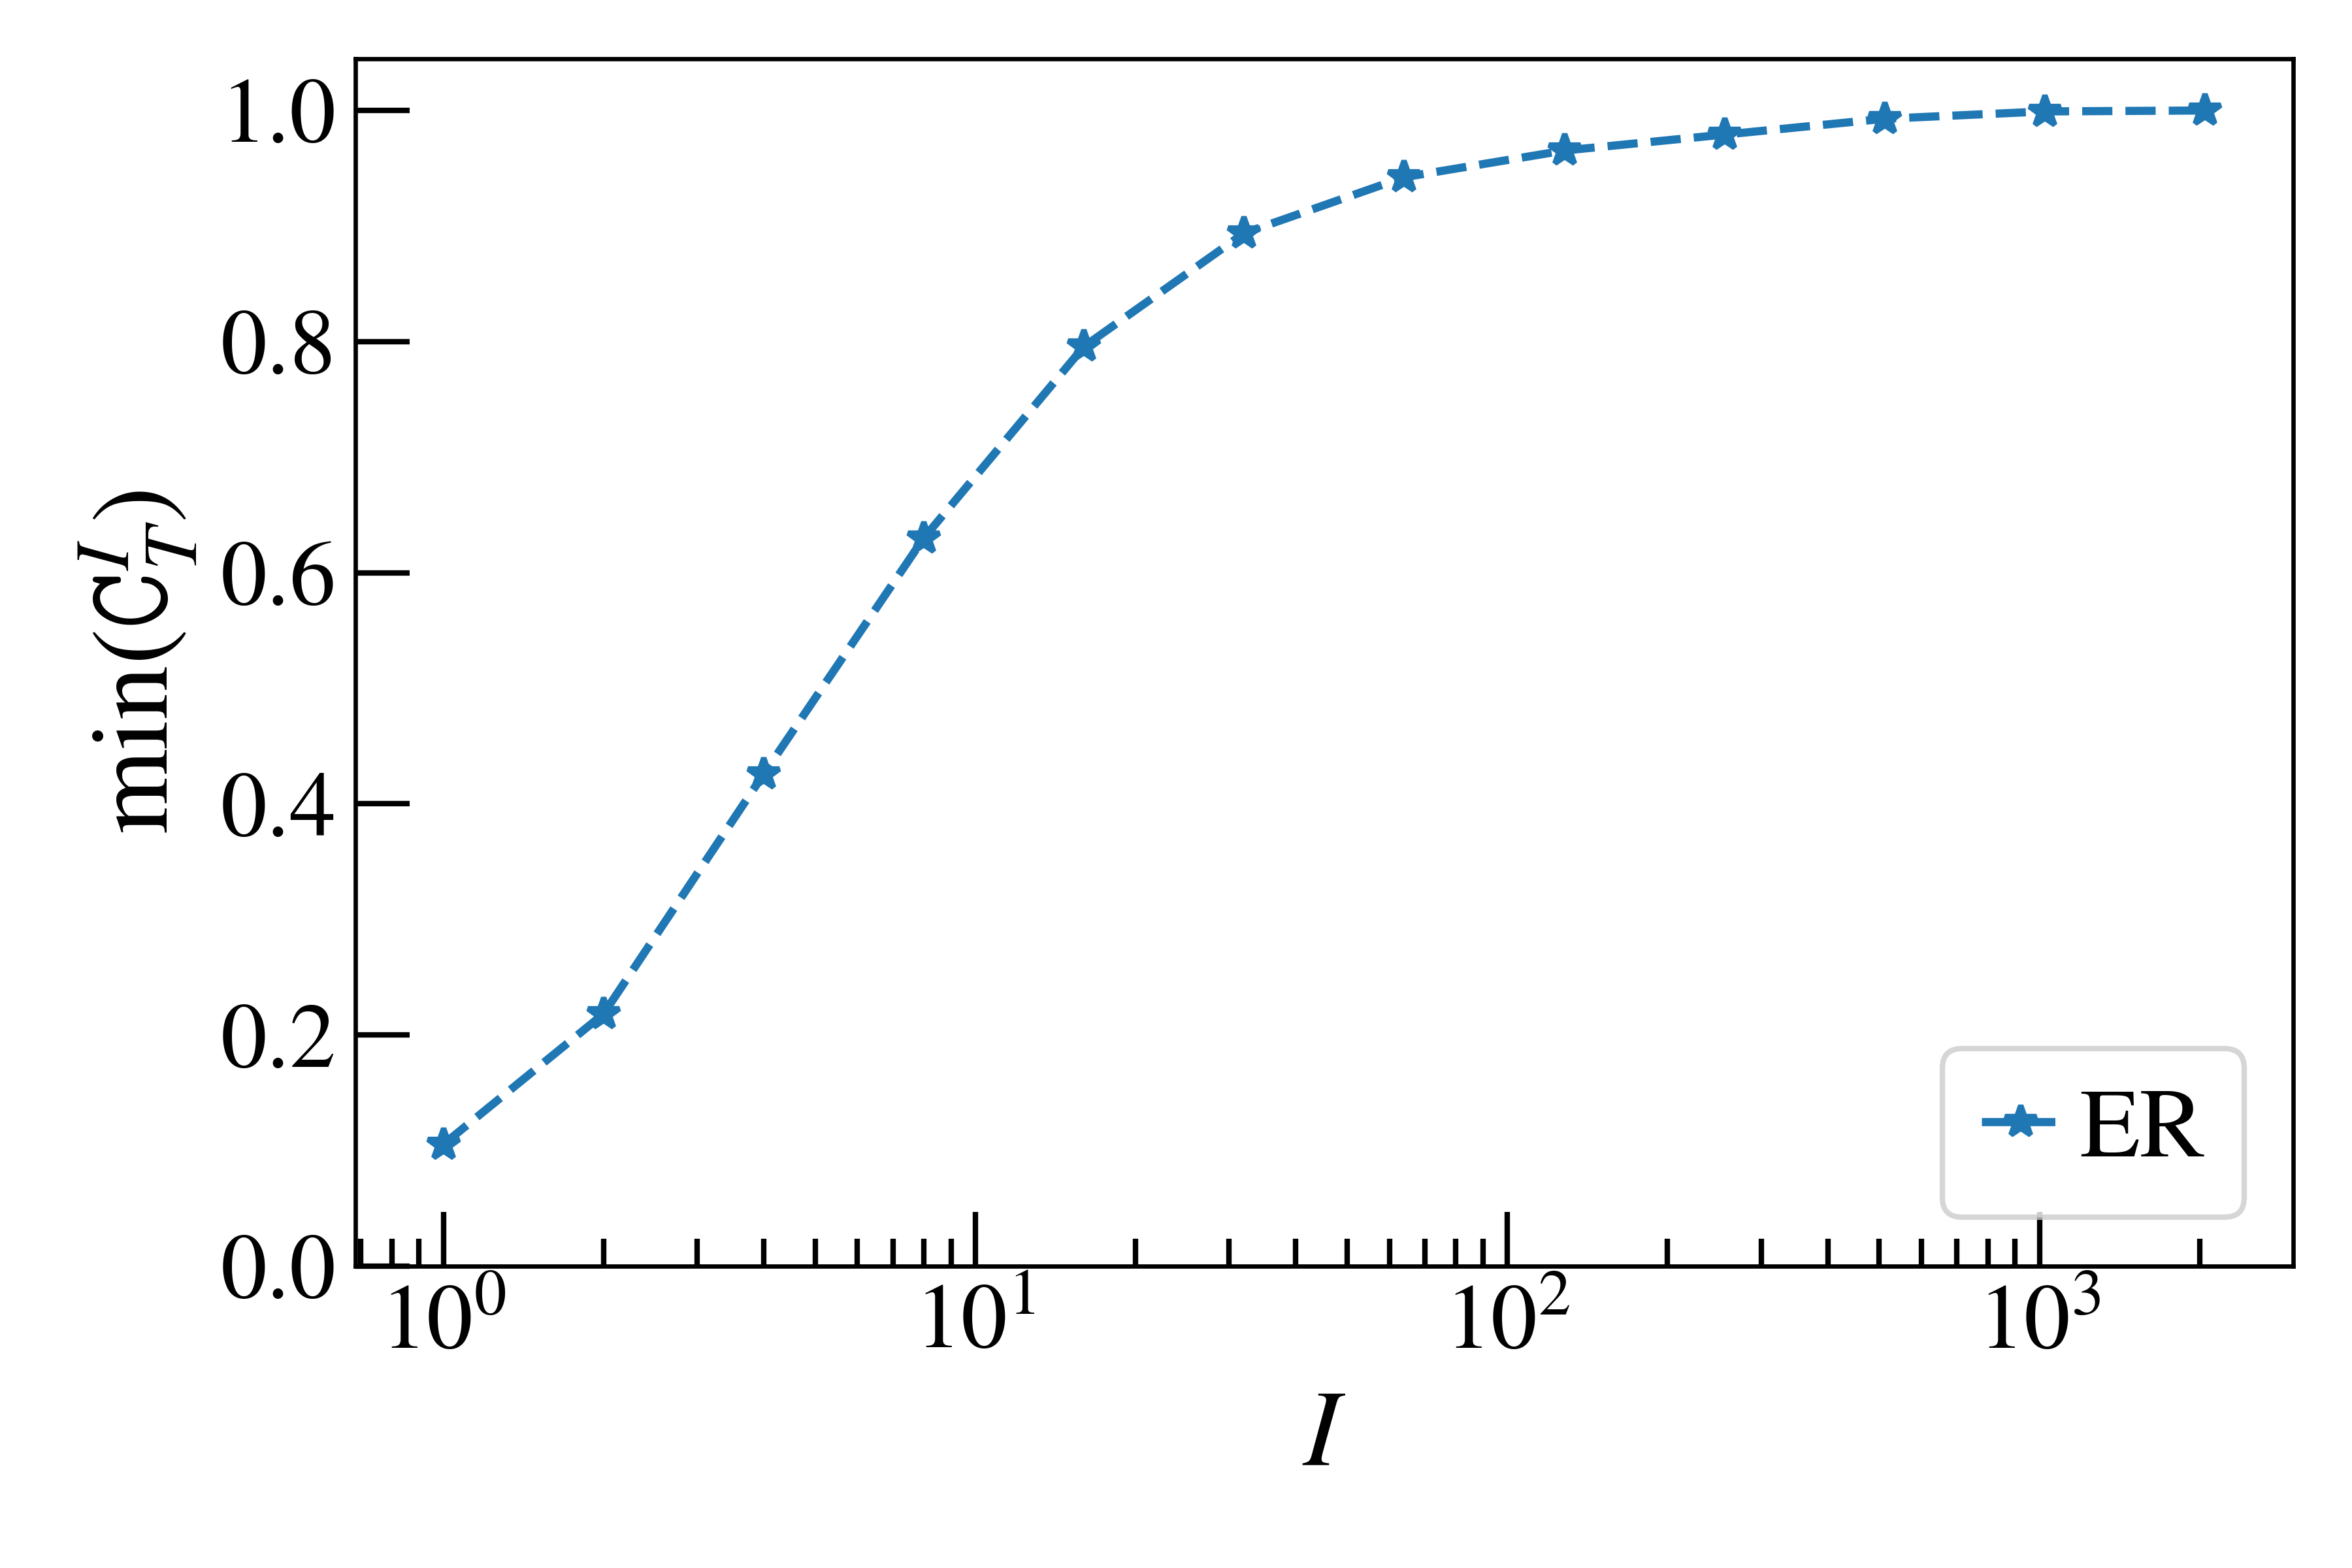
\includegraphics[width=0.48\textwidth]{fig/rnd_min_line.png}

\caption{\label{fig:SBMcf} 
Density of the accessibility matrix and
generalized causal fidelity for artificially generated random temporal network with two blocks with $N_1=N_2=50$ nodes and edge probabilities $q_{11}=0.001 $ and $q_{22}=0.00005$ as a function of the temporal network length $T$ for different number of aggregation intervals $I$.
The vertical lines show the analytical estimators $T_c$ (blue) and $T_f$ (red) for each block.
% Lower panel: Minima of the generalized causal fidelity $\mathtt{C}^I_T$ at different aggregation intervals $I$ for ER and SBM temporal networks with two blocks.
% \fla{N=..., T=..., q=...}
% \fla{add (4-5) curves for different $N$}
}
\end{figure}

Before considering more realistic degree distributions, it is instructive to see the effect of well defined temporal communities using the same temporal network model in two separate blocks. The two blocks do not interact, i.e. there are no inter-block edges. Further, they differ in their activity, meaning that the edge-probabilities within the two blocks differ.  
Each snapshot is the realization of a stochastic block model (SBM) with two blocks of equal size $(N_1=N_2)$ and edge probability  $q_{11},q_{22},q_{12},q_{21}$ with $q_{11}\neq q_{22}$ and $q_{12}=q_{21}=0$.  Each block can be seen as an individual random temporal network as above, but the two are represented in the same network. Thus, we can use the previous results obtained for Poisson random network, eq. \ref{eq:TC1}  and eq.  \ref{eq:TC2}, for each block separately by using the respective intra-block edge probability.  

In the upper panel of Fig.~\ref{fig:SBMcf} we show the accessibility density and the generalized causal fidelity with the analytical estimators $T_c$ and $T_f$ for both blocks. The results are fore
$N_1=N_2=50$ nodes and edge probabilities $q_{11}=0.001 $ and $q_{22}=0.00005$.
Since the two blocks follow a different activity rate, the emergence of connected components does not happen uniformly in the whole network but at different times in each block. Compared to the ER temporal network, the different temporal community blocks result in a double-well for the generalized causal fidelity, as well as in a stair pattern for the density of the accessibility. 
As for the ER case, the analytical estimators $T_c$ and $T_f$ correctly identify the critical range when the lowest causal fidelity is obtained for  the two blocks.

We conclude that the emergence of connectedness in a aggregated temporal network might happen at different ranges of $T$ for different communities and thus, for a given temporal network length $T$, the goodness of representation must not hold uniformly over the whole network but might differ between communities depending on their activity.   
% Fig.~\ref{fig:rndmin} also shows the expected worst case behavior of $\mathtt{C}^I_T$ for this more general model, showing  again that an initial increase of $I$ substantially reduces the information loss but the marginal effect decreases rapidly.



\subsection{\label{sec:EDSresults}
Scale-free random networks}

To test the solidity of the results obtained for Poisson degree distributions and to understand the influence of network topology on the generalized causal fidelity, we consider temporal networks with a scale-free (SF) degree distributions \cite{calda}. 
The probability for a node to have degree $k$ is $P(k)\sim k^{-\gamma}$, for constant $\gamma$. 
First, we generate a power-law degree sequence  $\{k_1,k_2,...,k_N\}$, and then we draw for each temporal snapshot a graph. Each snapshot is constructed using the Chung-Lu model \cite{chung2002connected}, which gives each edge $(u,v,t)$ from node $u$ to node $v$  in snapshot $t$ the probability $q_{uv} = k_u k_v/\sum_i k_i$, where $k_i$ is the expected degree of node $i$. This model gives each node $i$ in expectation the degree $k_i$, i.e., in expectation the degree sequence $\{k_1,k_2,...,k_N\}$ is realized in each snapshot.
For a perfectly SF network with exponent $\gamma$ we have $\braket{k (\gamma)} = (1-\gamma) (k_M^{2-\gamma}-1)/((2-\gamma)(k_M^{1-\gamma}-1))$, where $k_M$ is the maximum degree in the network.
Then for large networks, where finite size effects are negligible, the analytical expression $q(\gamma) = \braket{k(\gamma)}/N$, which explicitly depends on $\gamma$, can be used. 



%As a case study, in the following we consider expected degree sequences that follow a \textit{scale-free distribution}, meaning that the probability of  node $i$ having expected degree $w_i=k$ is proportional to $k^{-\gamma}$, where $\gamma$ is a model parameter ($P(w_i=k)\sim k^{-\gamma}$) \cite{barabasi2003scale}. To build the temporal network, we created a scale-free expected degree sequence using the  $'powerlaw\_sequence(N,\gamma)'$ function from the $networkx$ python package (\cite{networkx}). Since by this function, each node has an expected degree of $w_i>1$, each snapshot would be highly active. To reduce this activity we shrink down the expected degree sequence by a factor of 150. The Chung Lu model is then applied to the shrunk scale-free degree sequences to get a network for each snapshot.If one now aggregates over $150$ time points, the aggregated temporal network has an expected degree sequence equivalent to the one created in the beginning.


\begin{figure}[]
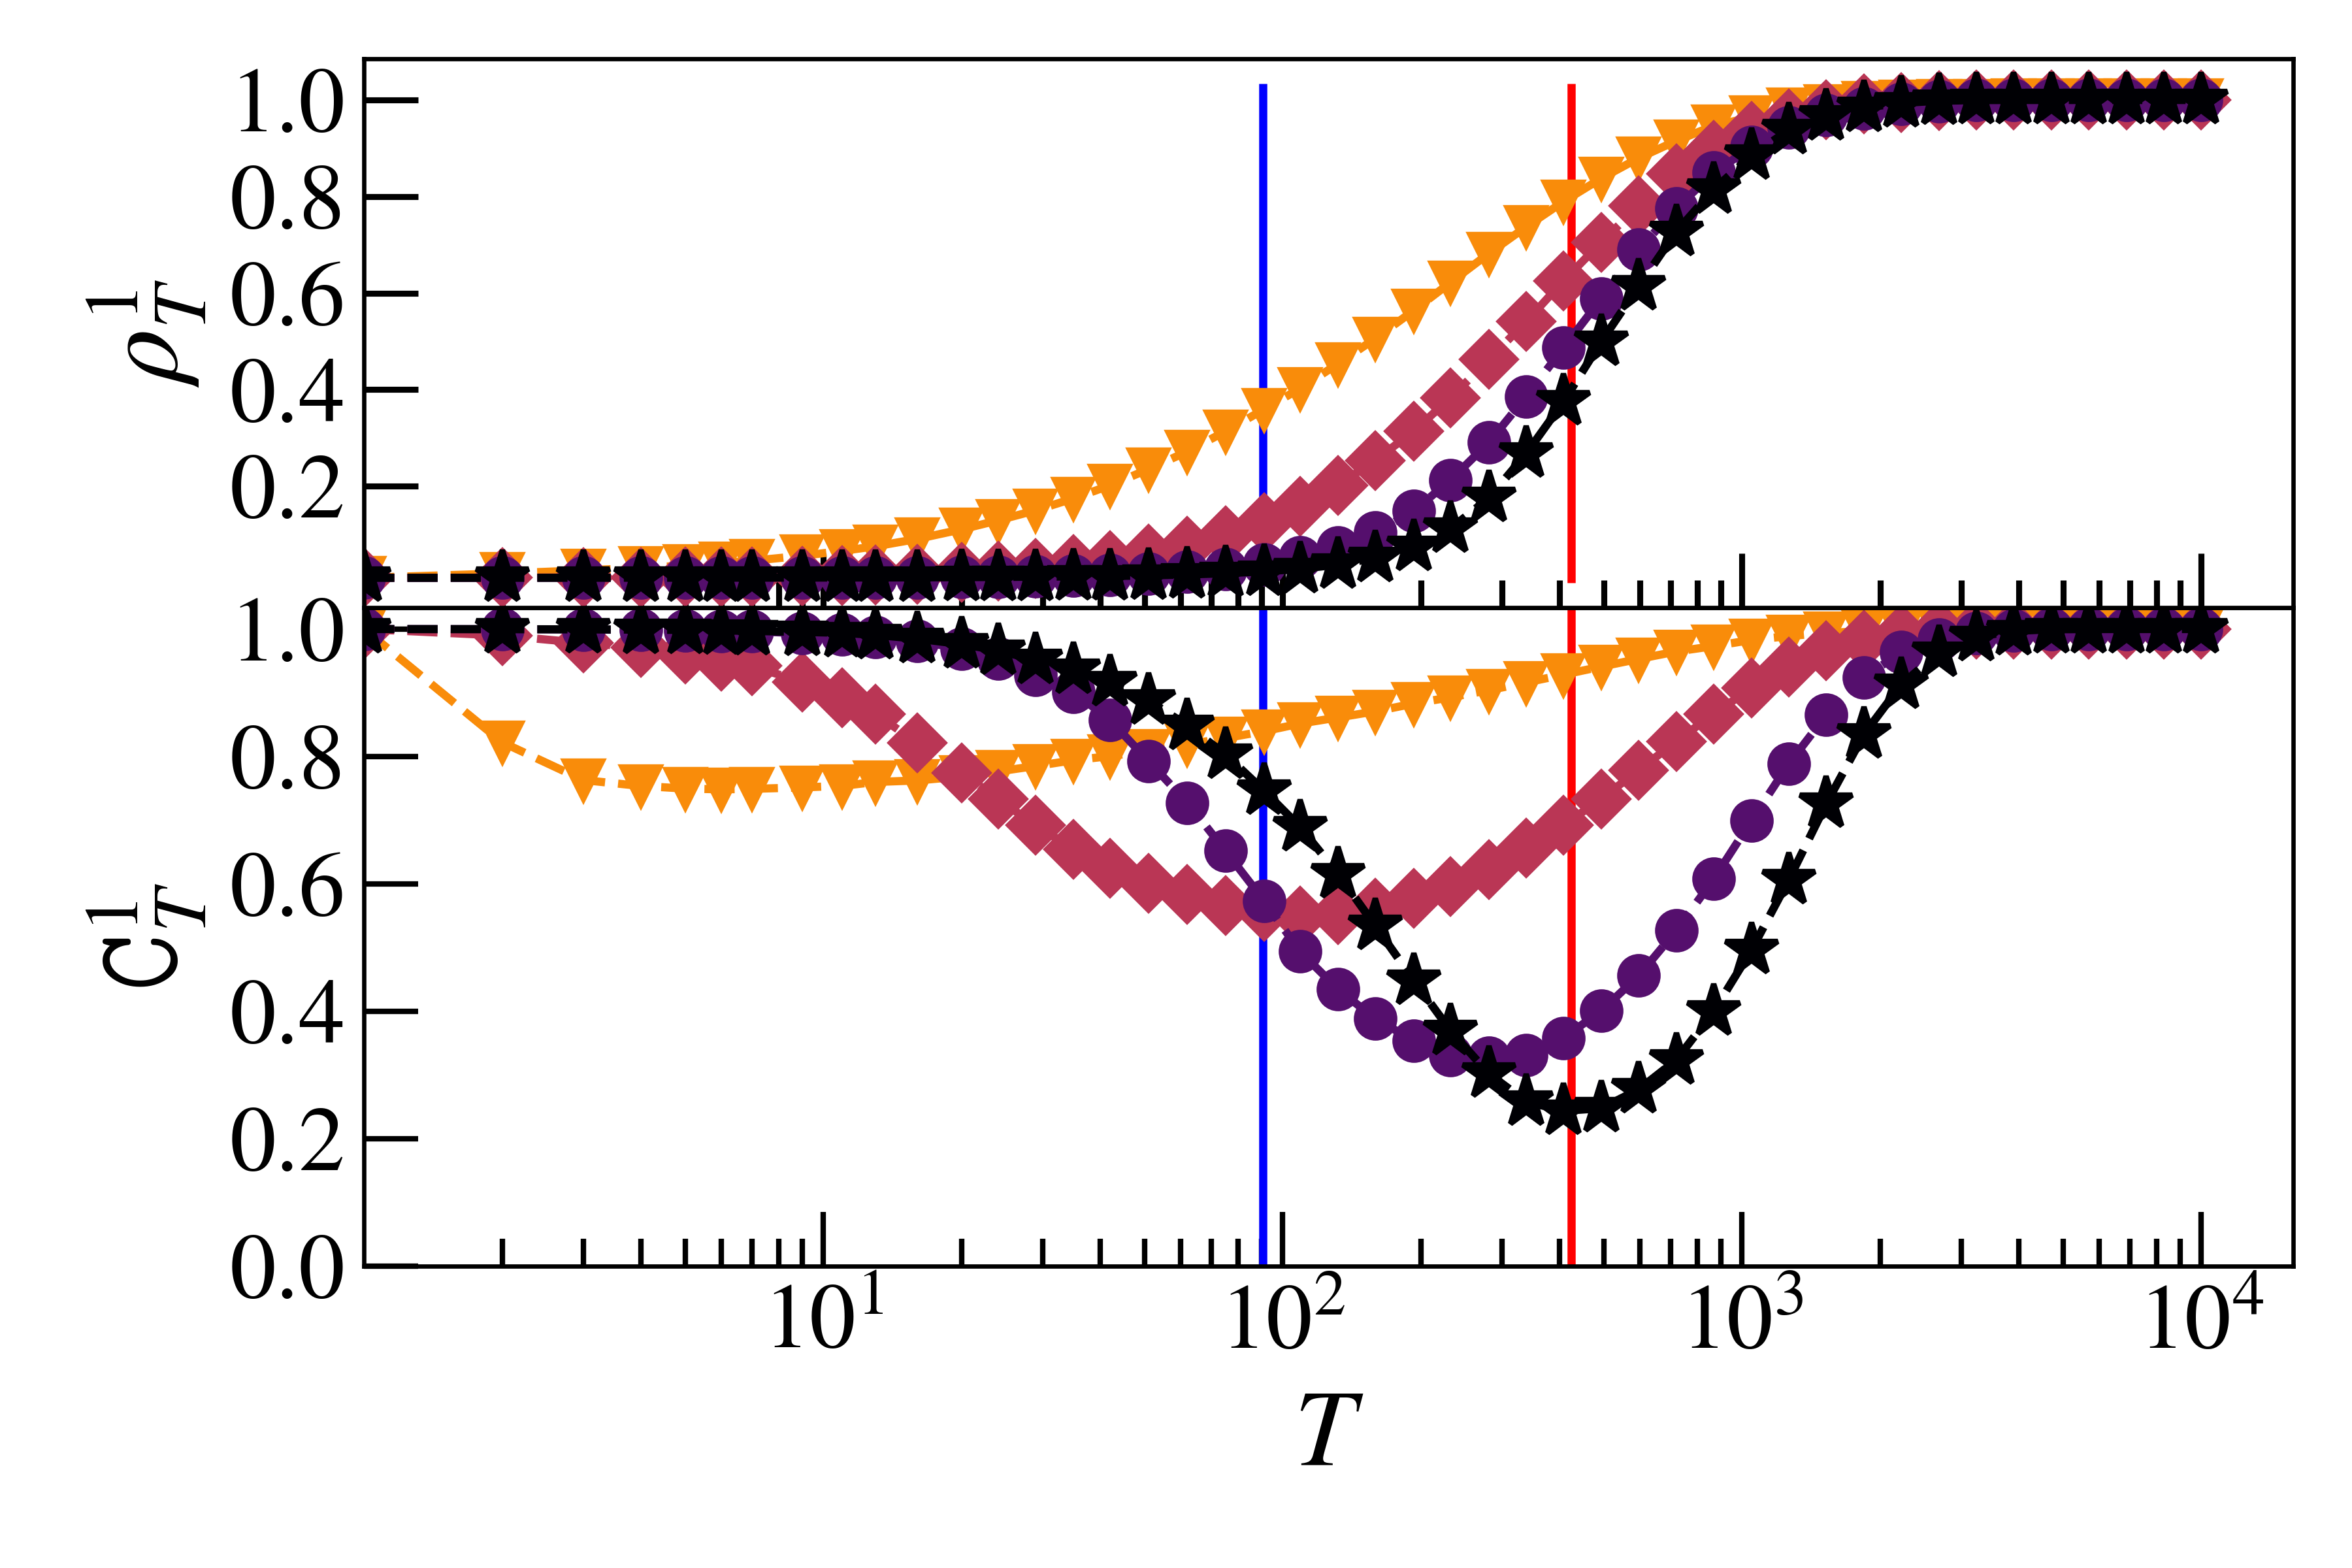
\includegraphics[width=0.48\textwidth]{fig/SF_cr_ana.png}
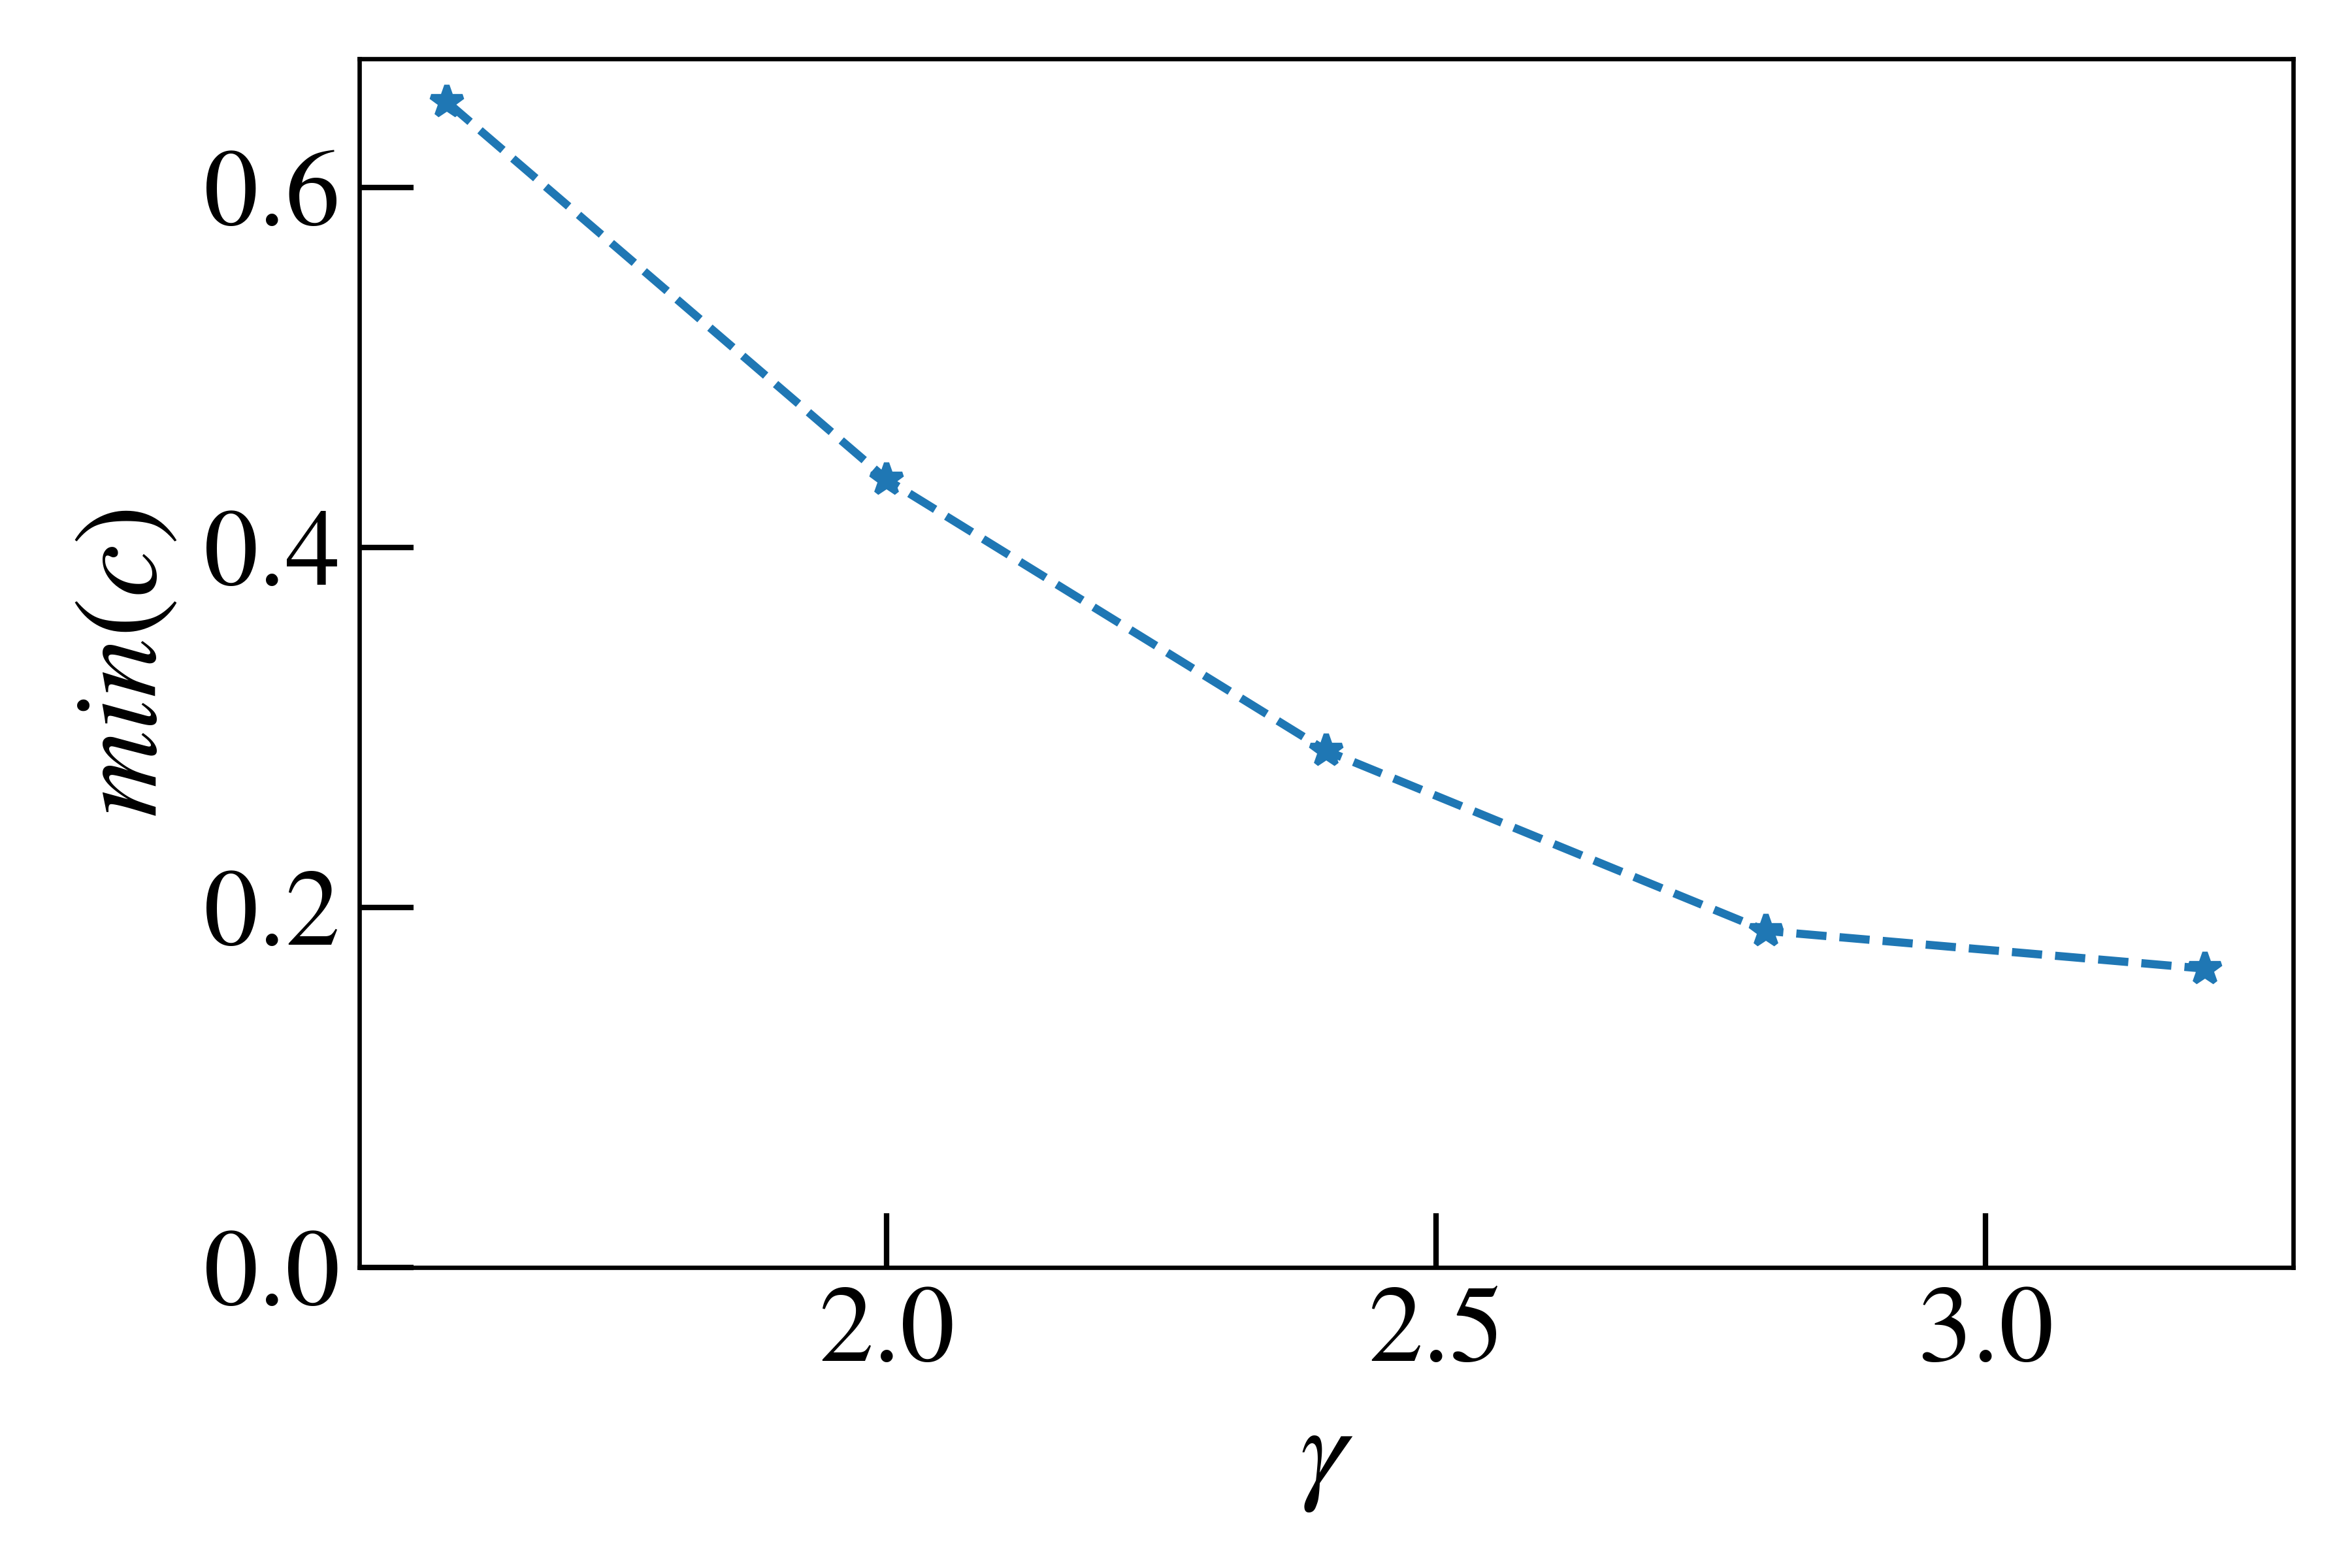
\includegraphics[width=0.48\textwidth]{fig/SF_min.png}

\caption{\label{fig:SFcf}
Upper panel: Results for SF networks with $N=100$ in the  $I=1$ case for different values of the degree distribution exponent $\gamma$. The vertical lines corresponds to the value $T_c(\gamma)={\ln(1-1/{N})}/{\ln(1-q(\gamma))}$ (blue line) and $T_f(\gamma)={\ln(1-{\ln(N)}/{N})}/{\ln(1-q(\gamma))}$ (red line) for the $\gamma=2.5$ case.
Lower panel: Minima of $\mathtt{C}^I_T$ as a function of number of aggregation intervals $I$ for SF networks with different values of $\gamma$ and ER network with the same value of $N$ and $q$.
}
\end{figure}

In the upper panel of Fig.~\ref{fig:SFcf} we show the causal fidelity $\mathtt{C}^I_T$ at $I=1$ for SF networks with $N=100$ and different values of the power-law exponent $\gamma$.
The analytical estimation of maximal information loss is given by eq.~\eqref{eq:TC1} and eq.~\eqref{eq:TC2}, using the average fraction of edges in each snapshot $q=\braket{k}/N$. 
By increasing $\gamma$, the worst case for information loss due to aggregation gets worse and shifts for higher values of $T$. Contrary,  low values of $\gamma$ give higher probabilities to nodes with higher degree, effectively freezing the interactions of active nodes around the hubs. The generalized causal fidelity decreases and reaches its minimum for lower values of $T$ and eventually saturates to its maximum value. 
% With lower $\gamma$ higher degrees are more likely, the network has more hubs. Since hubs are likely to connect to most nodes, they act as global connectors in the system and thereby improve the worst case. 
Thus, higher heterogeneity in the degree sequence of each aggregate correspond to best performance and lower information loss due to aggregation.

In the lower panel of Fig.~\ref{fig:SFcf} we show the minima of $\mathtt{C}^I_T$ as function of $I$ for different values of $\gamma$.
By considering few aggregation intervals, the expected worst case can be improved by a great margin. For further improvement, many more intervals need to be considered (note log scale). Thus, lifting the worst case to a reasonable level is well possible with some intervals, but getting a close to perfect representation takes many more intervals, i.e. increasing the number of intervals brings a diminishing improvement of the causal fidelity.
For low aggregation interval number, we obtain good improvement from the worse case for high values of $\gamma$. The gap shrinks as $\gamma$ is lowered, showing that heterogeneity and the presence of hubs in temporal networks yields an improved performance with respect to information loss when fewer intervals are used.
The limiting case $\gamma=3$, when each snapshot start to behave as an homogeneous graph, gives quantitatively similar behavior as for ER networks. 







\subsection{\label{sec:EMPresults}Real Temporal Networks}

\begin{figure*}[]
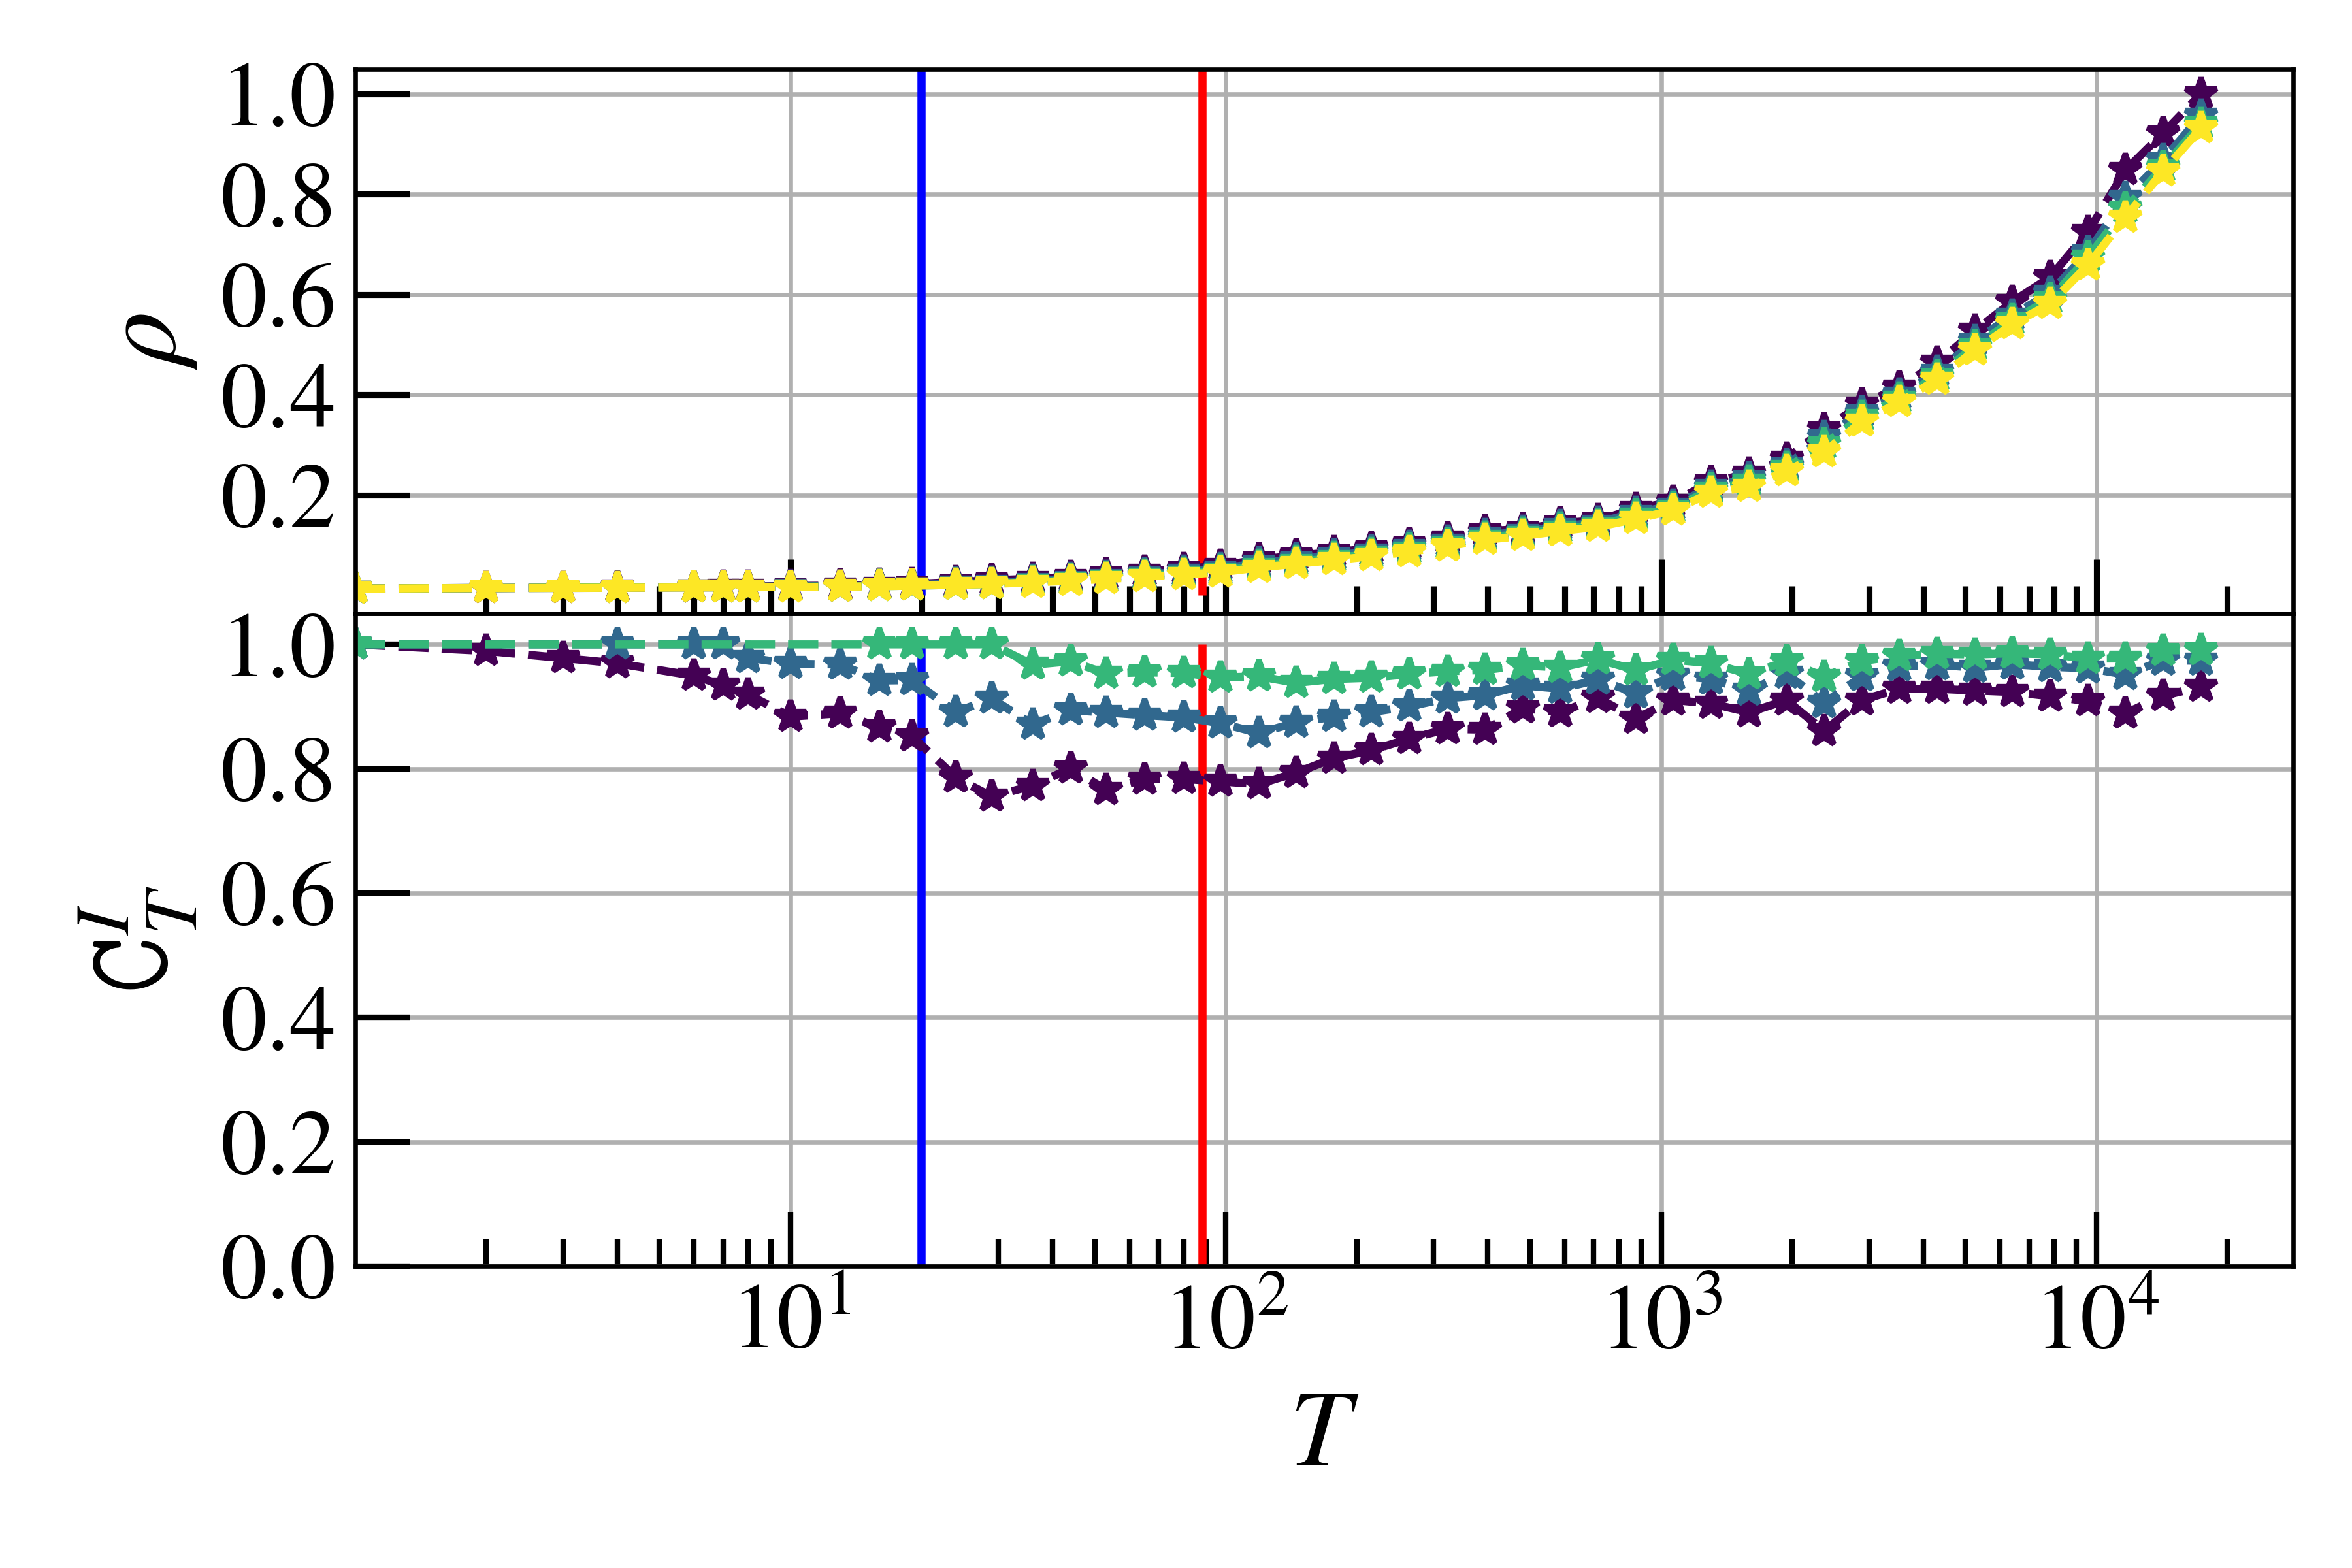
\includegraphics[width=0.48\textwidth]{fig/hospital_cr_ana.png}
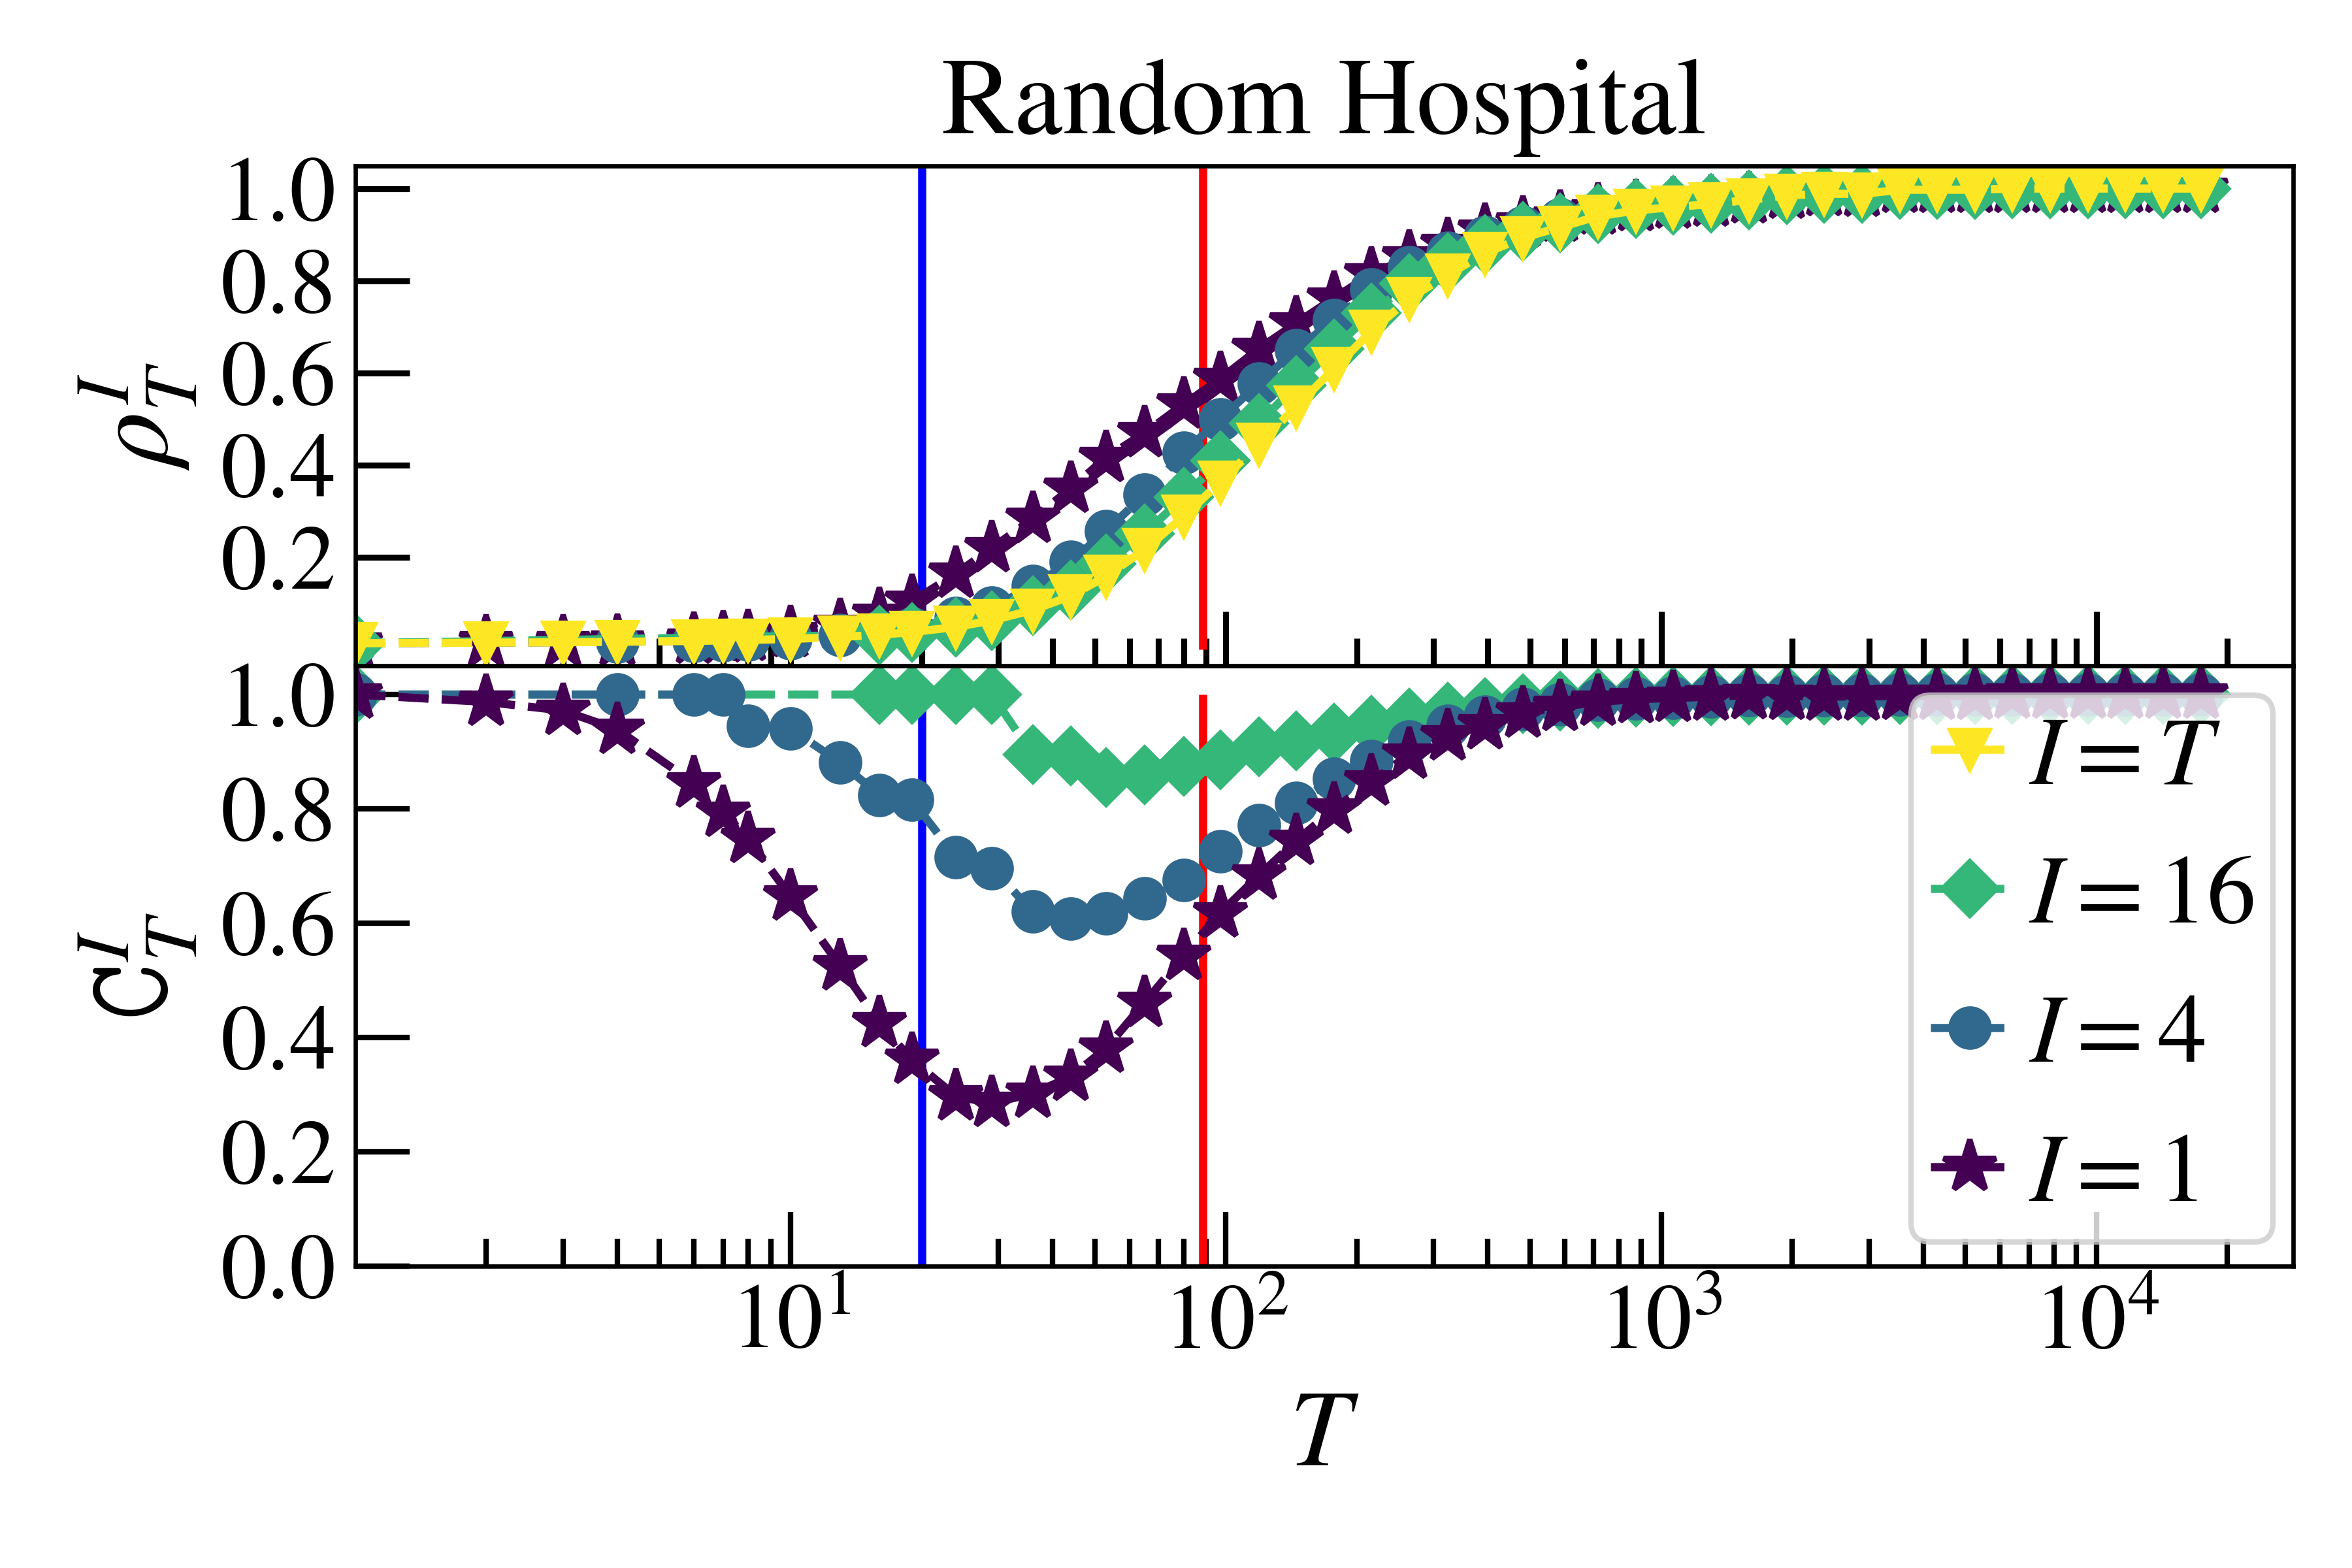
\includegraphics[width=0.48\textwidth]{fig/hospital_ET_cr_ana_leg.png}
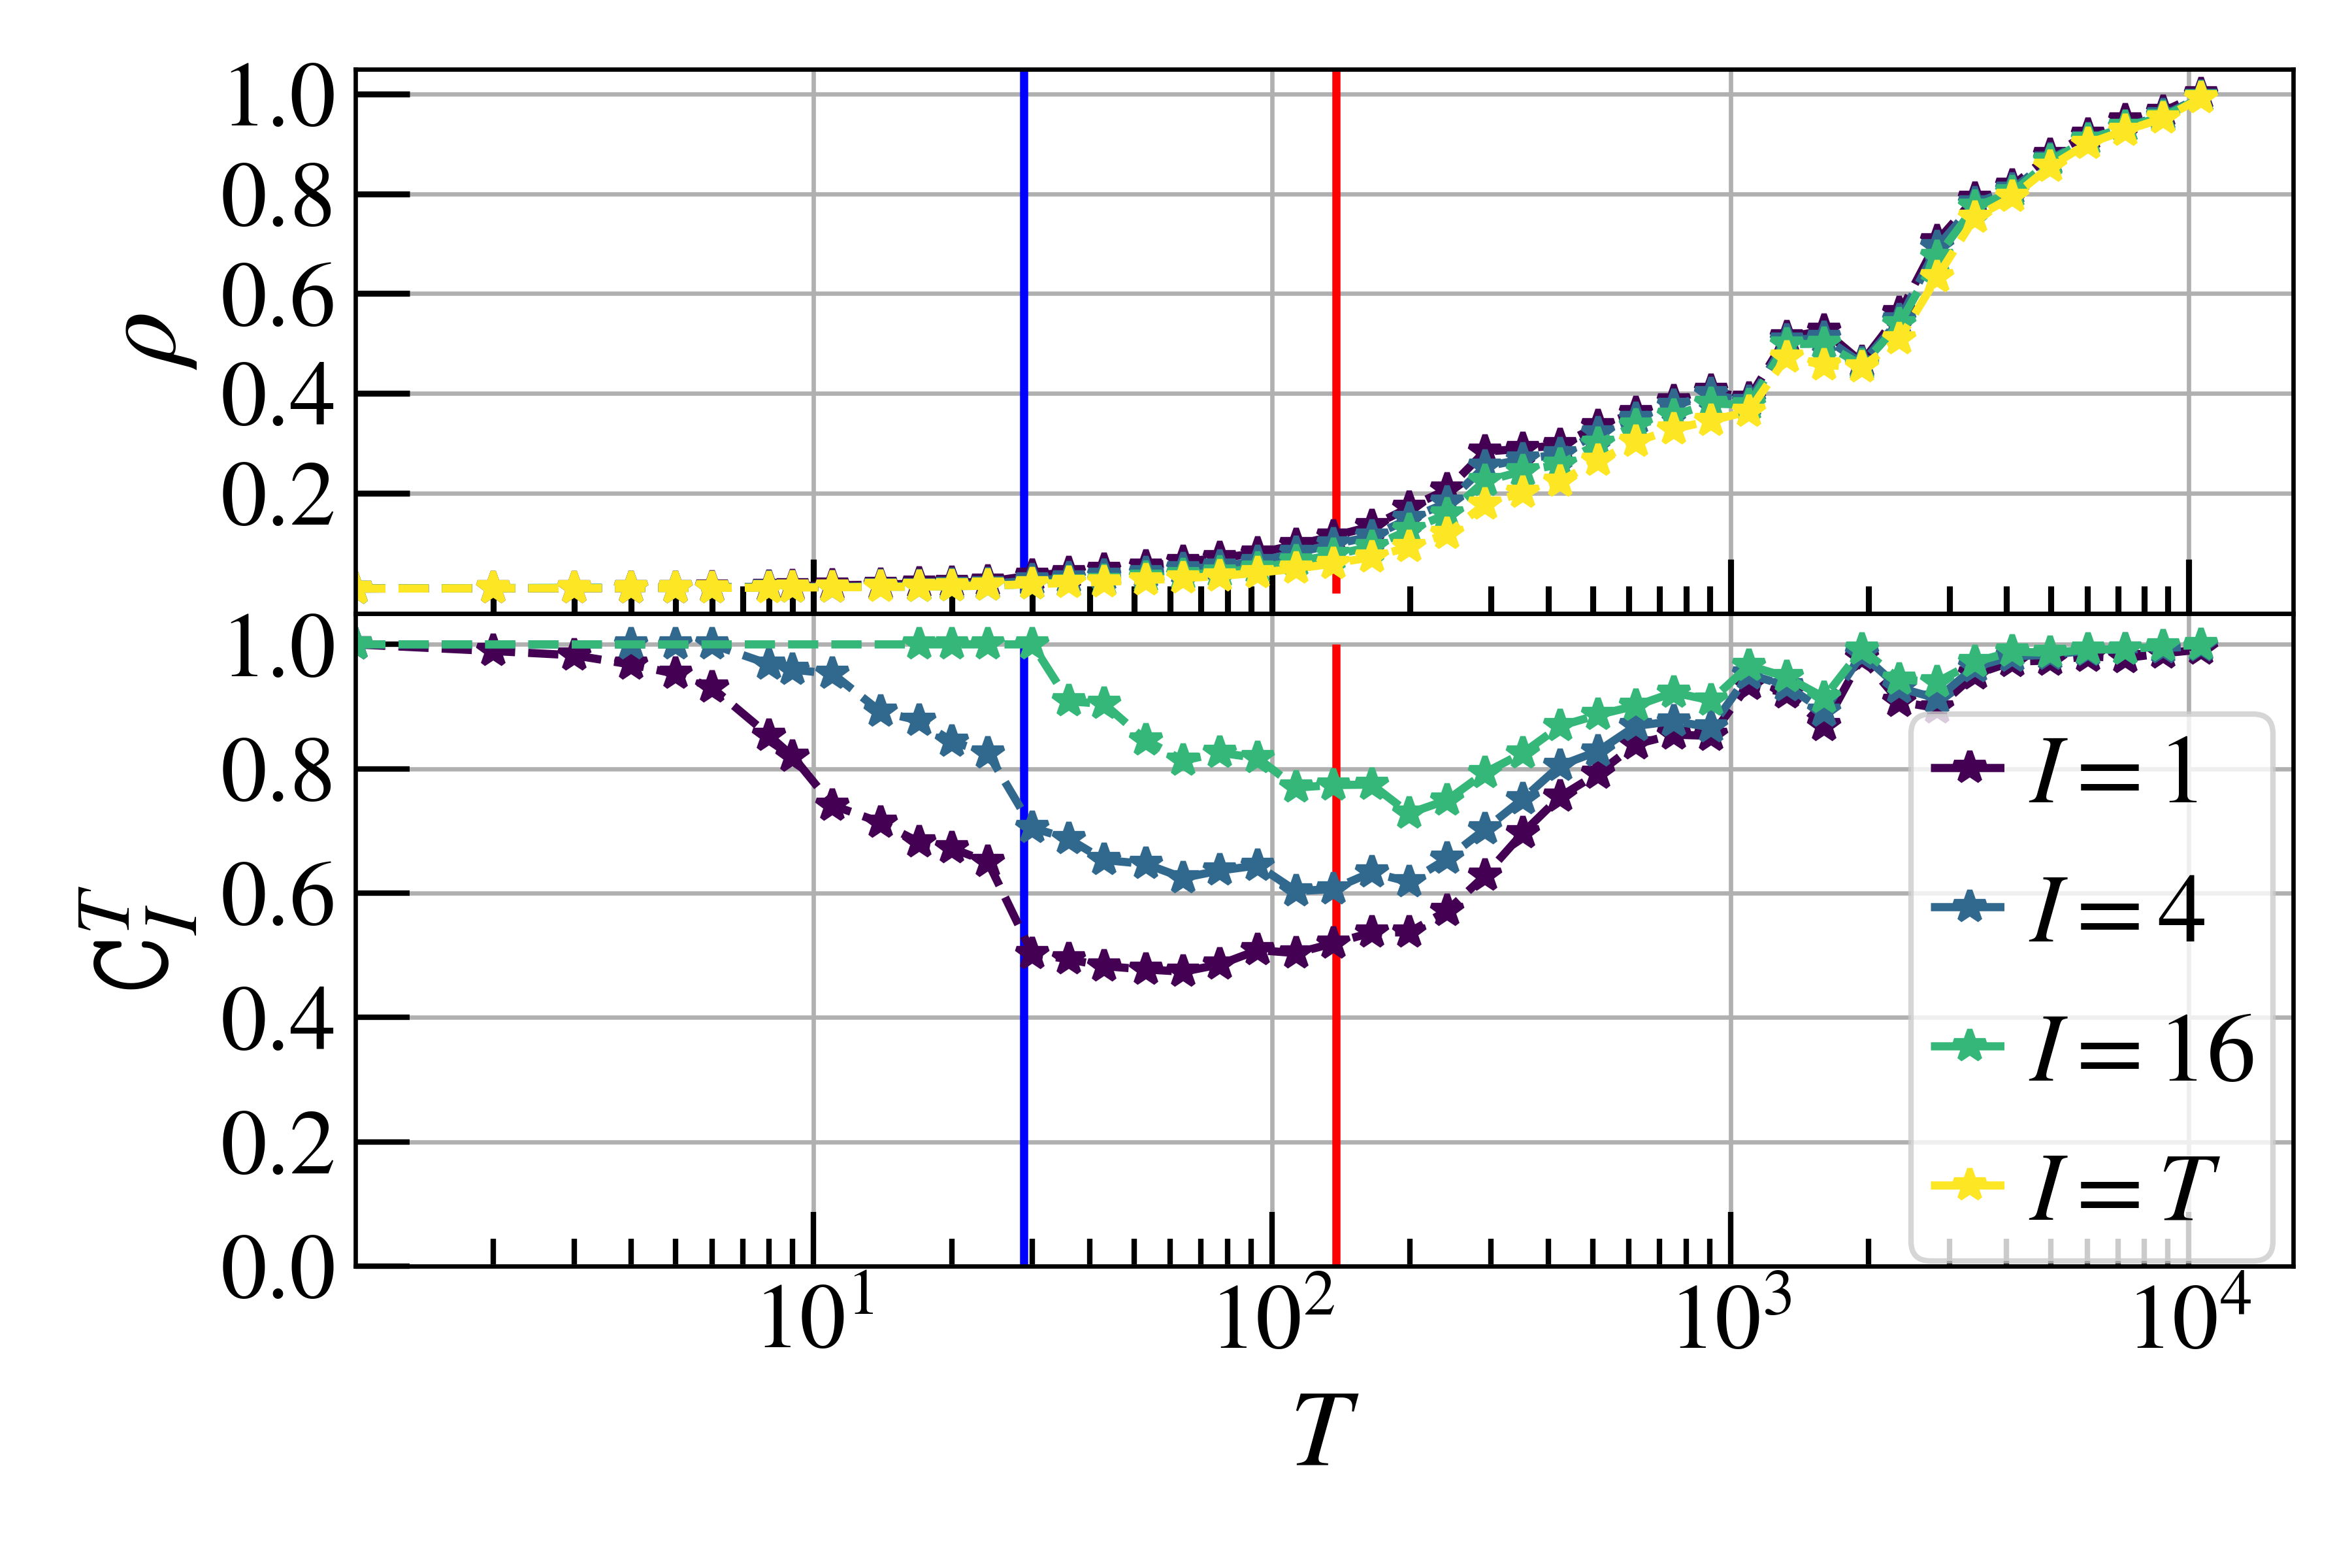
\includegraphics[width=0.48\textwidth]{fig/hypertext_cr_ana.png}
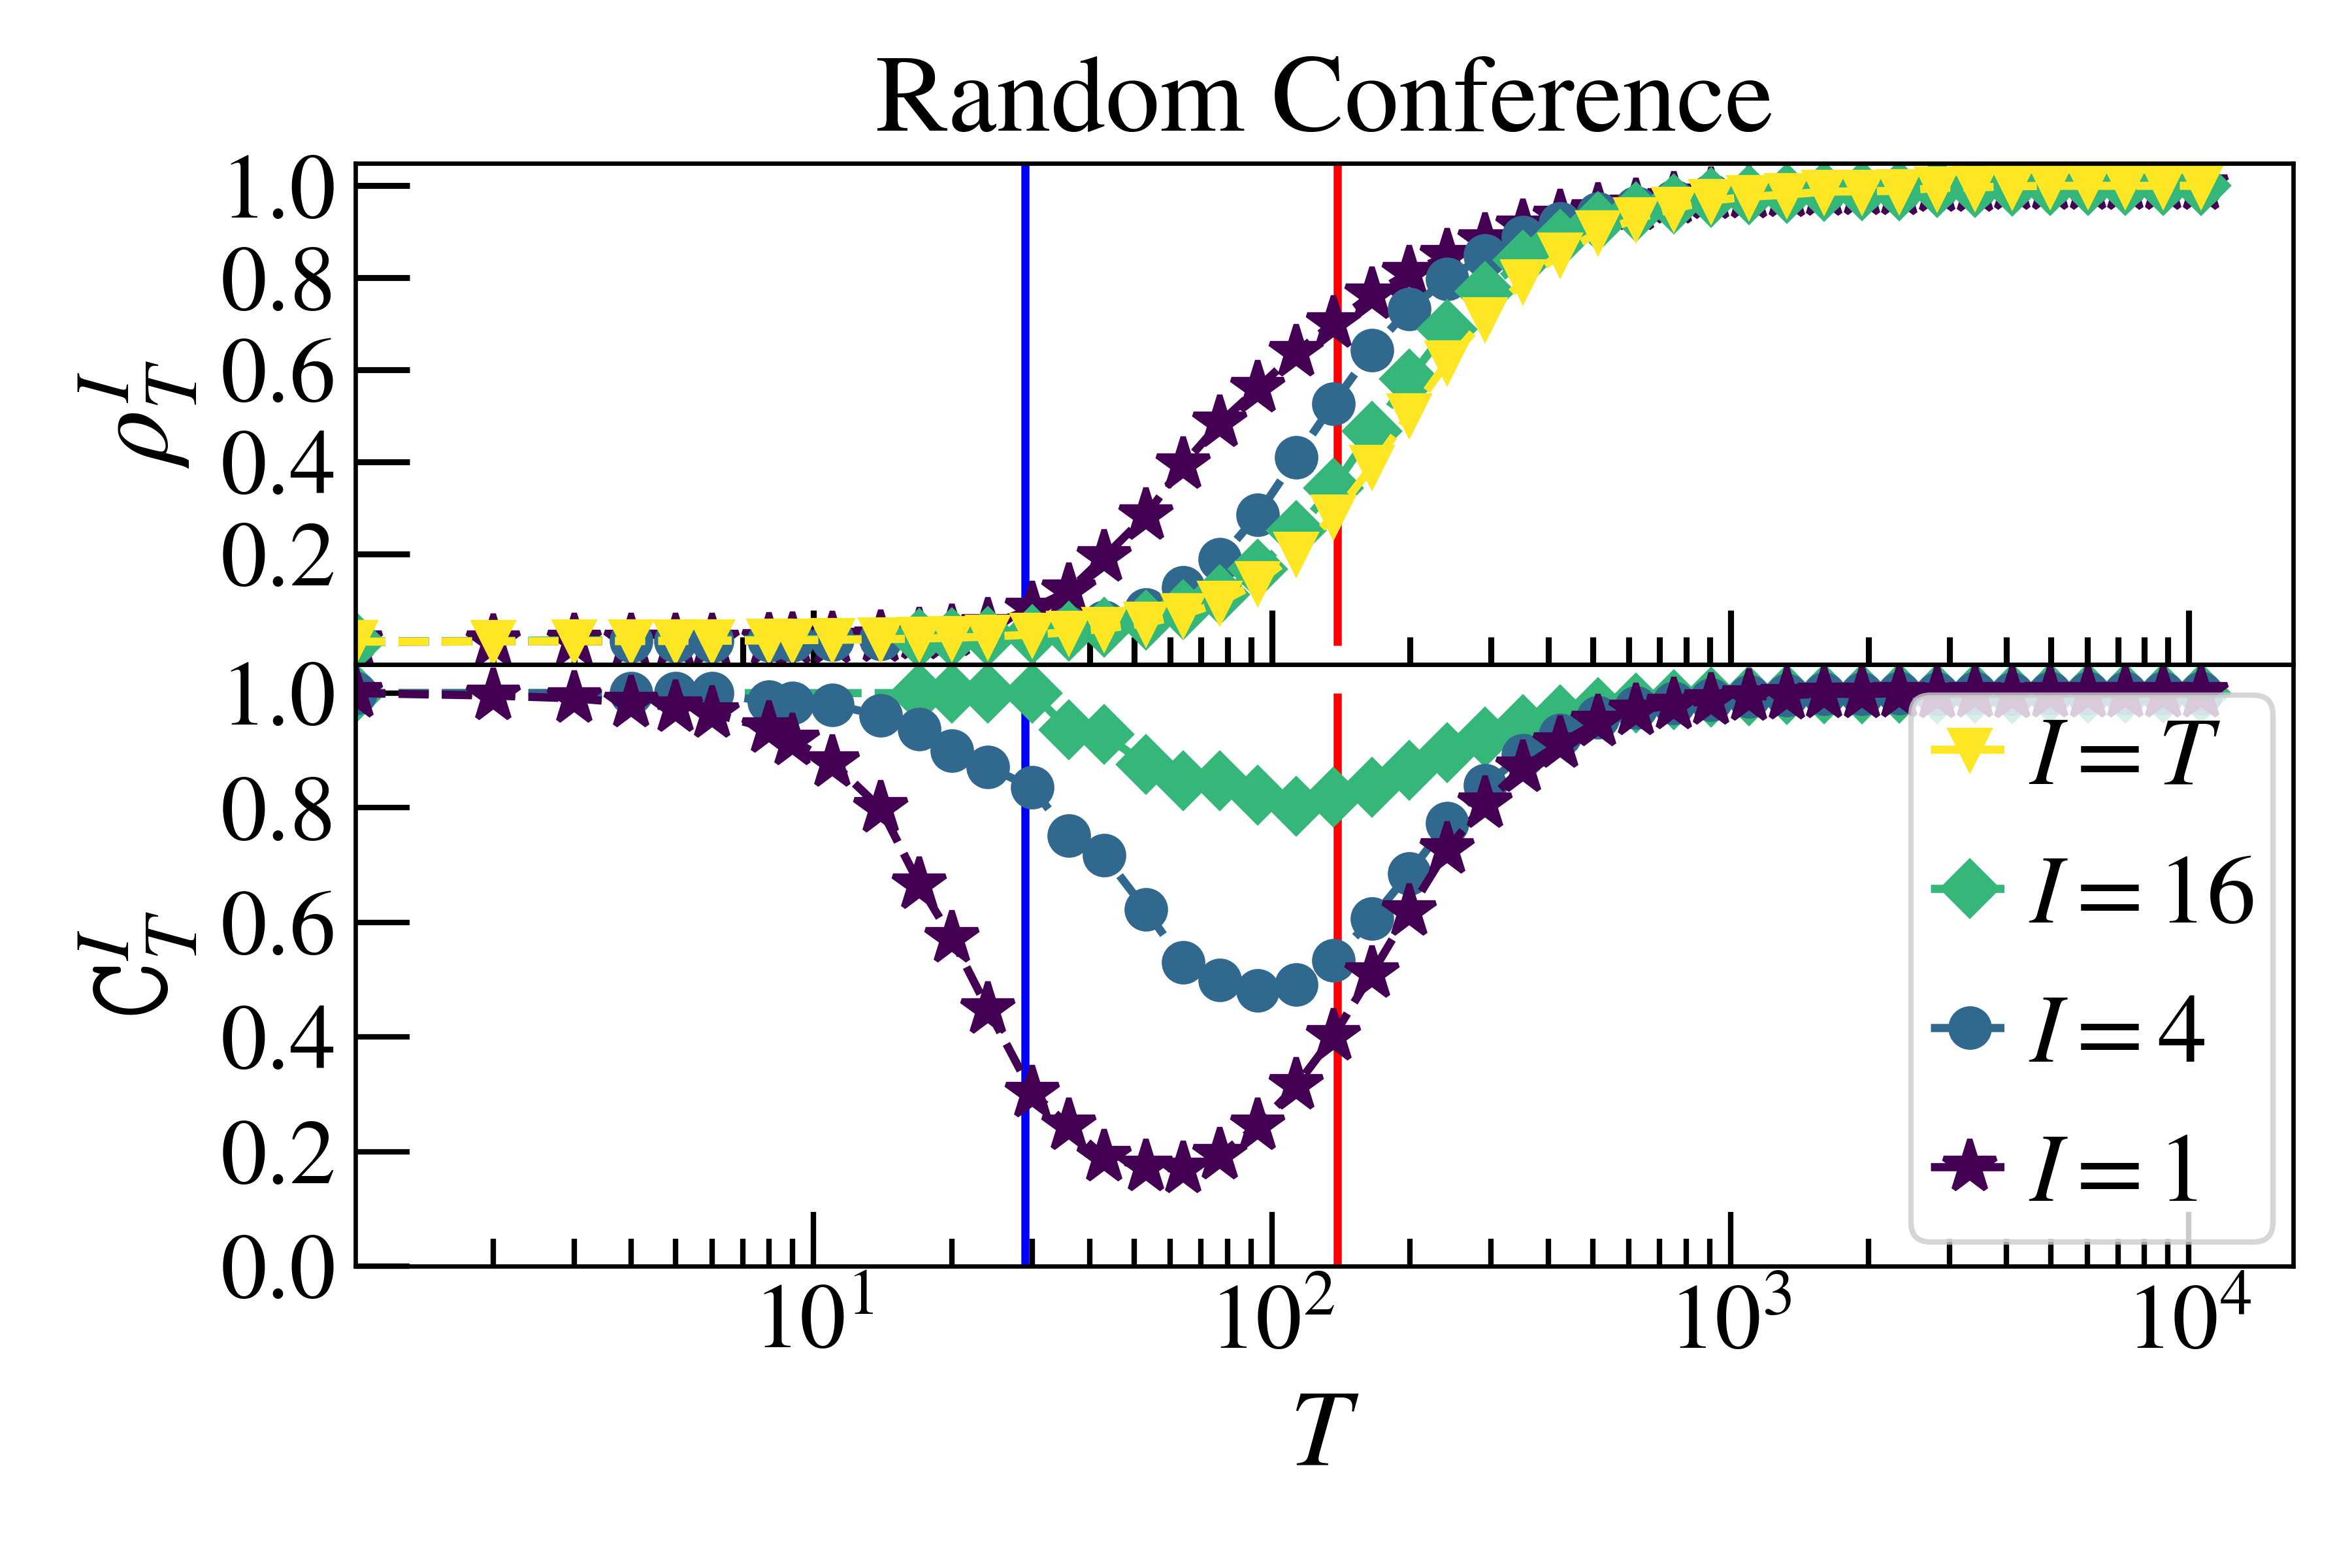
\includegraphics[width=0.48\textwidth]{fig/hypertext_ET_cr_ana_leg.png}
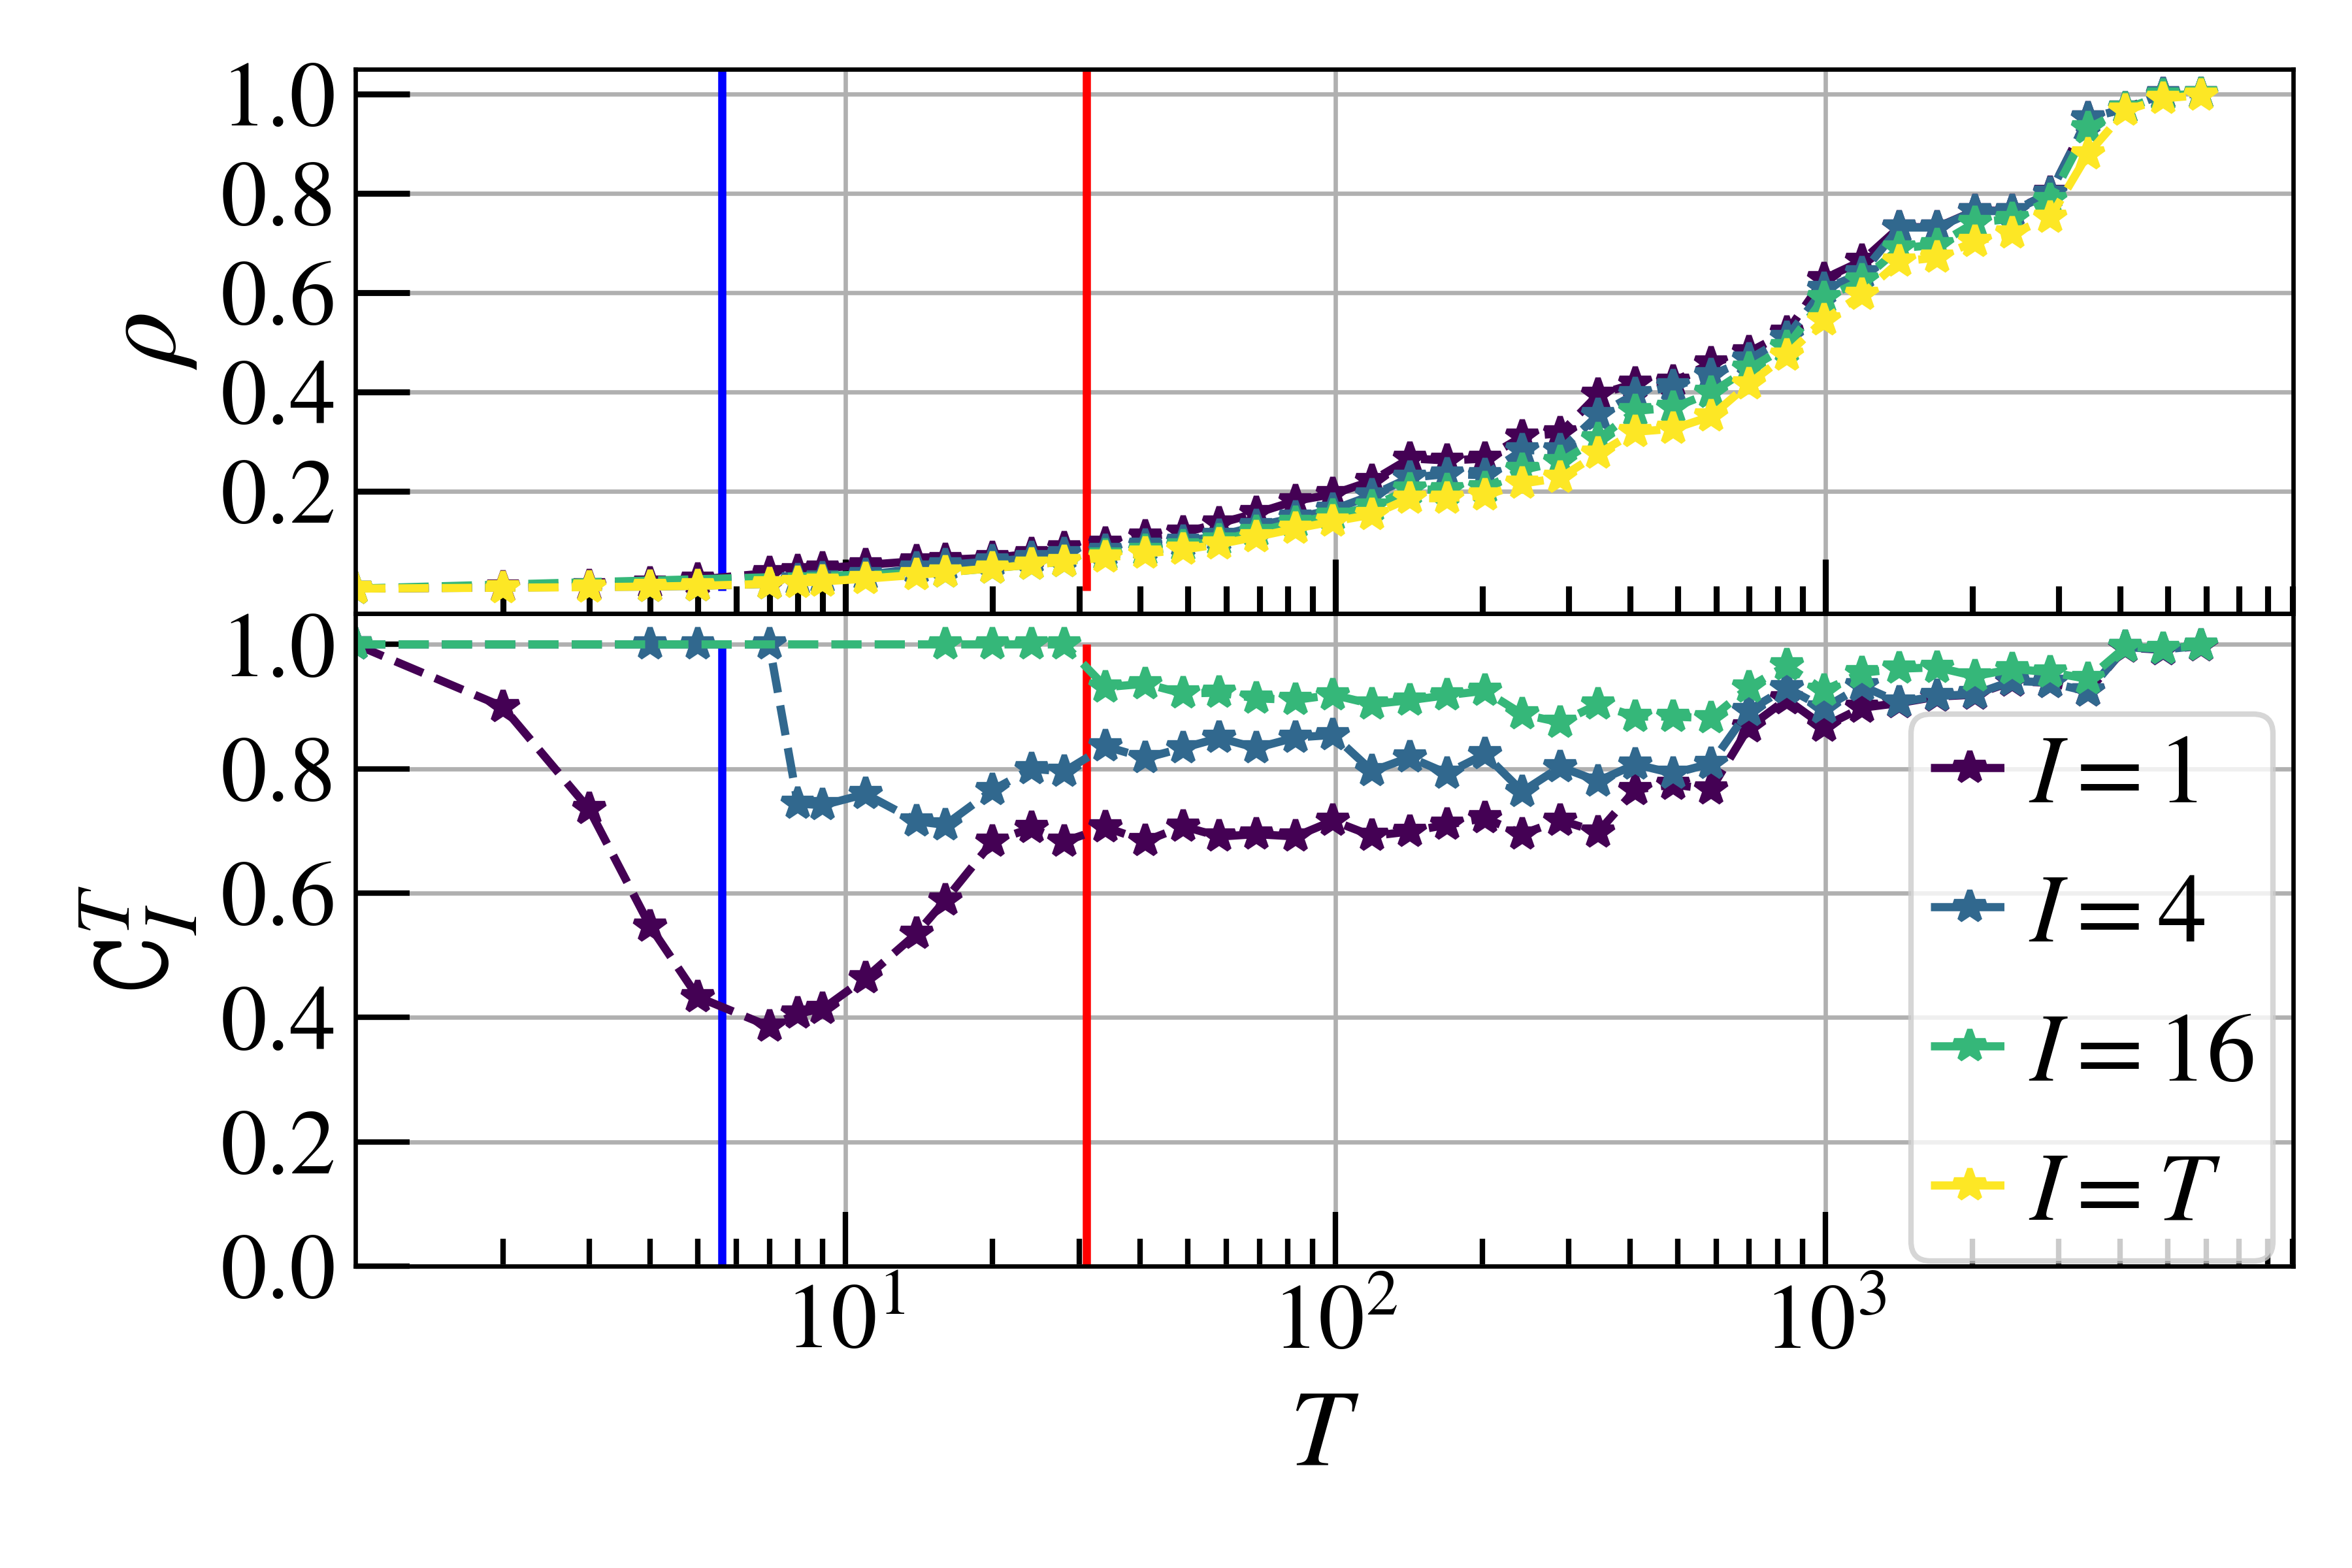
\includegraphics[width=0.48\textwidth]{fig/primaryschool_cr_ana.png}
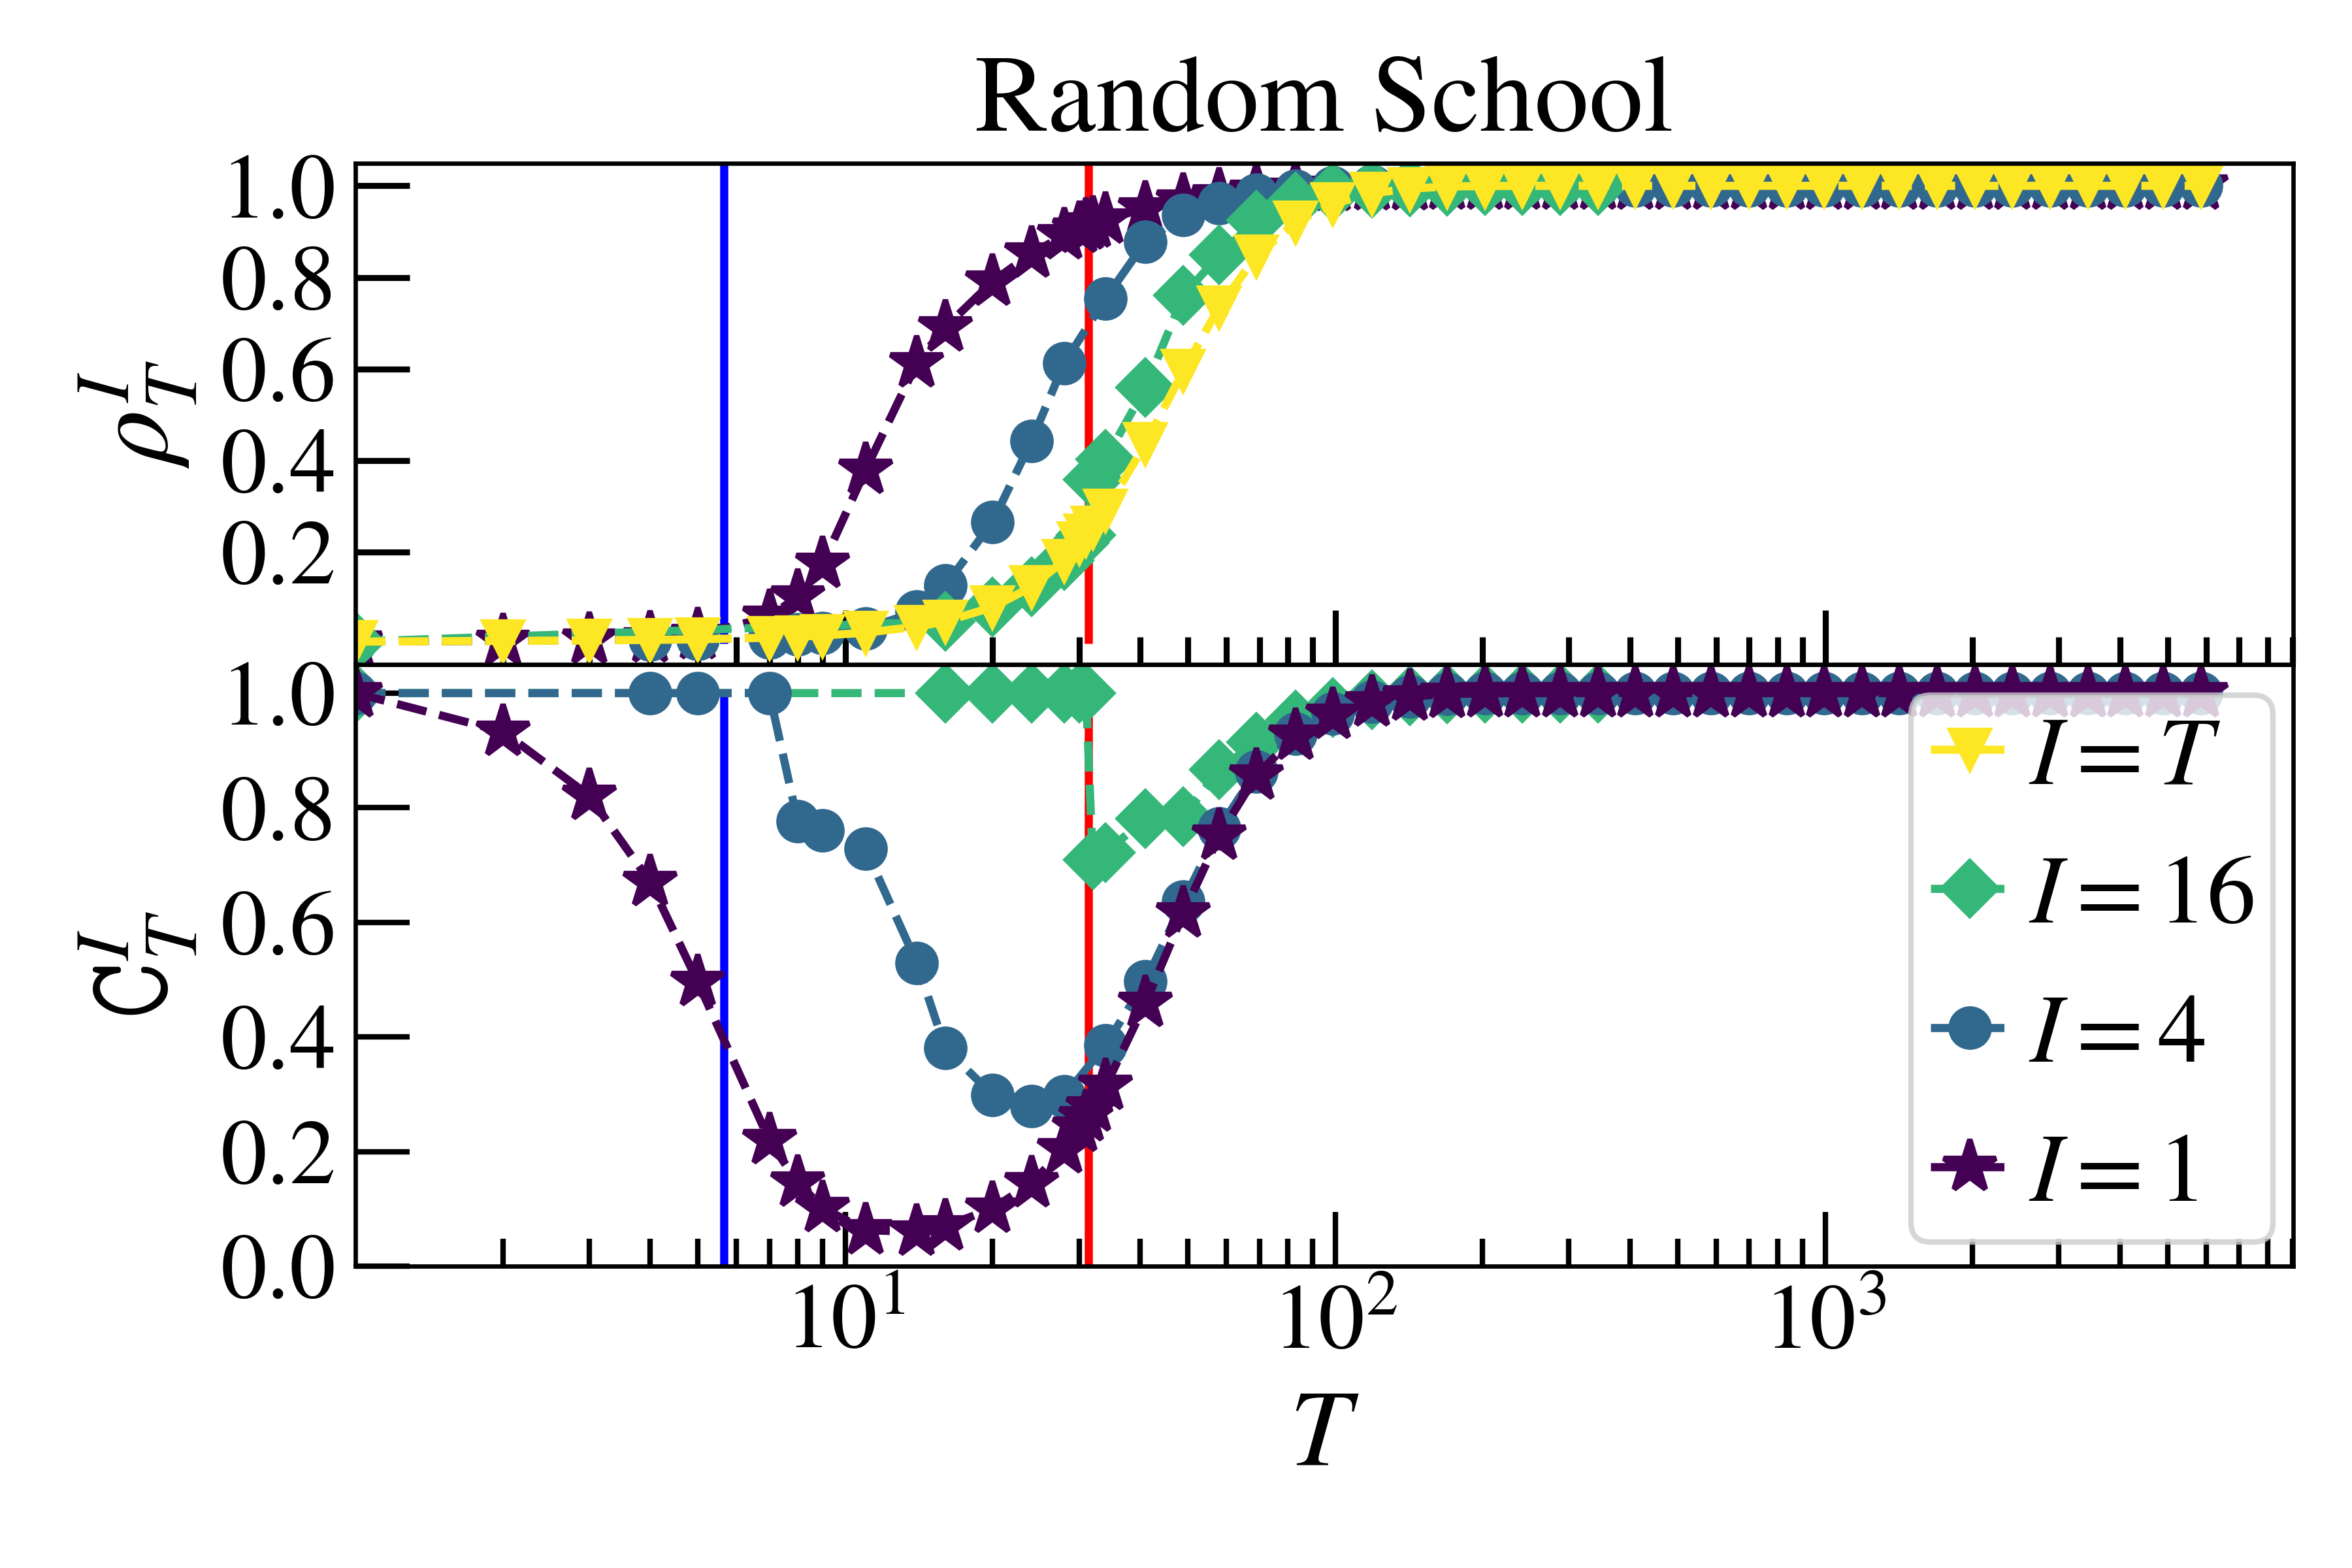
\includegraphics[width=0.48\textwidth]{fig/primaryschool_ET_cr_ana_leg.png}
\caption{\label{fig:dataPScf} 
Results for three temporal network datasets. 
In each panel we show the density of the accessibility matrix $\rho(\mathcal{P}^I_T)$ and generalized causal fidelity $\mathtt{C}^I_T$.
The vertical lines mark the analytical estimation for the range of the maximal information loss $T_c$ (blue) and $T_f$ (red).
The left panels show the results for the original datasets and the right panels show the results for the same networks with randomized temporal edges.  Different colors refer to different aggregation interval values. For the properties of the different datasets, see Table \ref{tab:datastats}.
}
\end{figure*}


In this section we show the results for three temporal network datasets containing contacts between individuals over time in three different contexts. We sample and analyze temporal networks of different lengths $T$ from the datasets and analyze these samples. Then, we create randomized temporal networks from these datasets by randomizing the edges in time. Since the datasets have a fixed given length, also our analysis is limited by this length, i.e. we can not sample and analyze any temporal network longer then the length given by the dataset. 


\begin{table}[h!]
\centering
\begin{tabular}{lrrrrrrr}
\hline
 Dataset       &   $N$  &    $E$&    $\mathcal{T}$ &  $\Delta t$ &   {$\langle k \rangle$}   & $\mathcal{G}$  & $\min (\mathtt{C}^1_T)$ \\ %&  {$\mathtt{C}^1_\mathcal{T}$}
\hline
Hospital       &       $75$ &    32424 &    17376 &    20s  &  864   & 0.28   &  0.75\\ %&  0.93
Conference      &      $113$ &    41636 &    10618 &    20s  &  368   & 0.26   &  0.47\\ %&  0.99 
School &                $242$ &   251546 &     5846 &    20s  & 1039   &  0.22  &  0.39\\  %&  0.99 
\hline
\end{tabular}
\caption{Statistical properties of the analyzed temporal networks. The different quantities are the number of nodes $N$, the total number of temporal edges $E$,  the total number of snapshots $\mathcal{T}$, the time unit between two consecutive snapshots $\Delta t$,  the average degree $\langle k \rangle$,  the minimum of the causal fidelity $\min (\mathtt{C}^1_T)$ between the temporal network and the full aggregated network and the Gini coefficient $\mathcal{G}$ of the degree distribution.\simon{I put minimum of $\mathtt{C}_T^1$ instead of $\mathtt{C}_\mathcal{T}^1$}
}
\label{tab:datastats}
\end{table}


For the numerical analysis, the following datasets are used:
(i) The \emph{Hospital} dataset contains contacts between patients and health-care workers in a hospital ward in Lyon over five days in 2010 \cite{hospital}.
(ii) The \emph{Conference} dataset contains contacts between attendees of the ACM Hypertext 2009 conference over 2.5 days \cite{hypertext}. 
(iii) The \emph{School} dataset contains contacts between children and teachers of a primary school in 2009 over two days \cite{primaryschool2,primaryschool1}. 
For all datasets, an undirected edge $(u,v,t)$ is present if person $u$ and person $v$ had an active contact in the time window $[t-20sec, t]$.
The relevant statistical properties of the datasets are reported in Table \ref{tab:datastats}.





In Fig.~\ref{fig:dataPScf} we show (left panels) the results for temporal networks sampled from the original dataset. As for synthetic networks, we find the characteristic valley containing the global minimum of causal fidelity. 
Contrary to synthetic networks, the saturation of the density of the accessibility graph is shifted at higher values of $T$. The vertical lines mark the theoretical estimators for the maximal information loss interval $T_c<T<T_f$. 
While the global minimum of casual fidelity  lies in that range consistently, the upper bound given by $T_f$ does not correspond to saturation of the accessibility density as for artificial networks. This mismatch can be explained in terms of the correlations between temporal edges that are present in real data.
By comparing with the randomized networks (right panels), the analytical estimators for maximal information loss consistently identify the minimum causal fidelity.

In Fig.~\ref{fig:dataMin} we plot the minima of $\mathtt{C}^I_T$ as function of $I$ for the original and randomized dataset, showing again a strongly diminishing marginal effects when increasing $I$.
For low interval numbers, the minima of the original datasets (upper panel) display a slow saturation compared to their randomized counterpart (lower panel).
The minima for the School dataset saturate faster compared to the other datasets. Thus, even if there is higher information loss for the worse case, there is substantial improvement obtained by considering only a few additional intervals.
For both the original and randomized datasets, the minima saturate approximately when more then $I=100$ aggregation intervals are used. This is quite surprising considering the large variation in the dataset lengths $\mathcal{T}$ for these datasets, see Table \ref{tab:datastats}. 
\fla{comment on dataset degree heterogeneity}
\simon{WATCH OUT: lower minimum could be explained by two things: - \textit{more heterogeneity}, but also \textit{more nodes} since as we saw for ER: more Nodes $\rightarrow$ lower minimum}




\begin{figure}[]
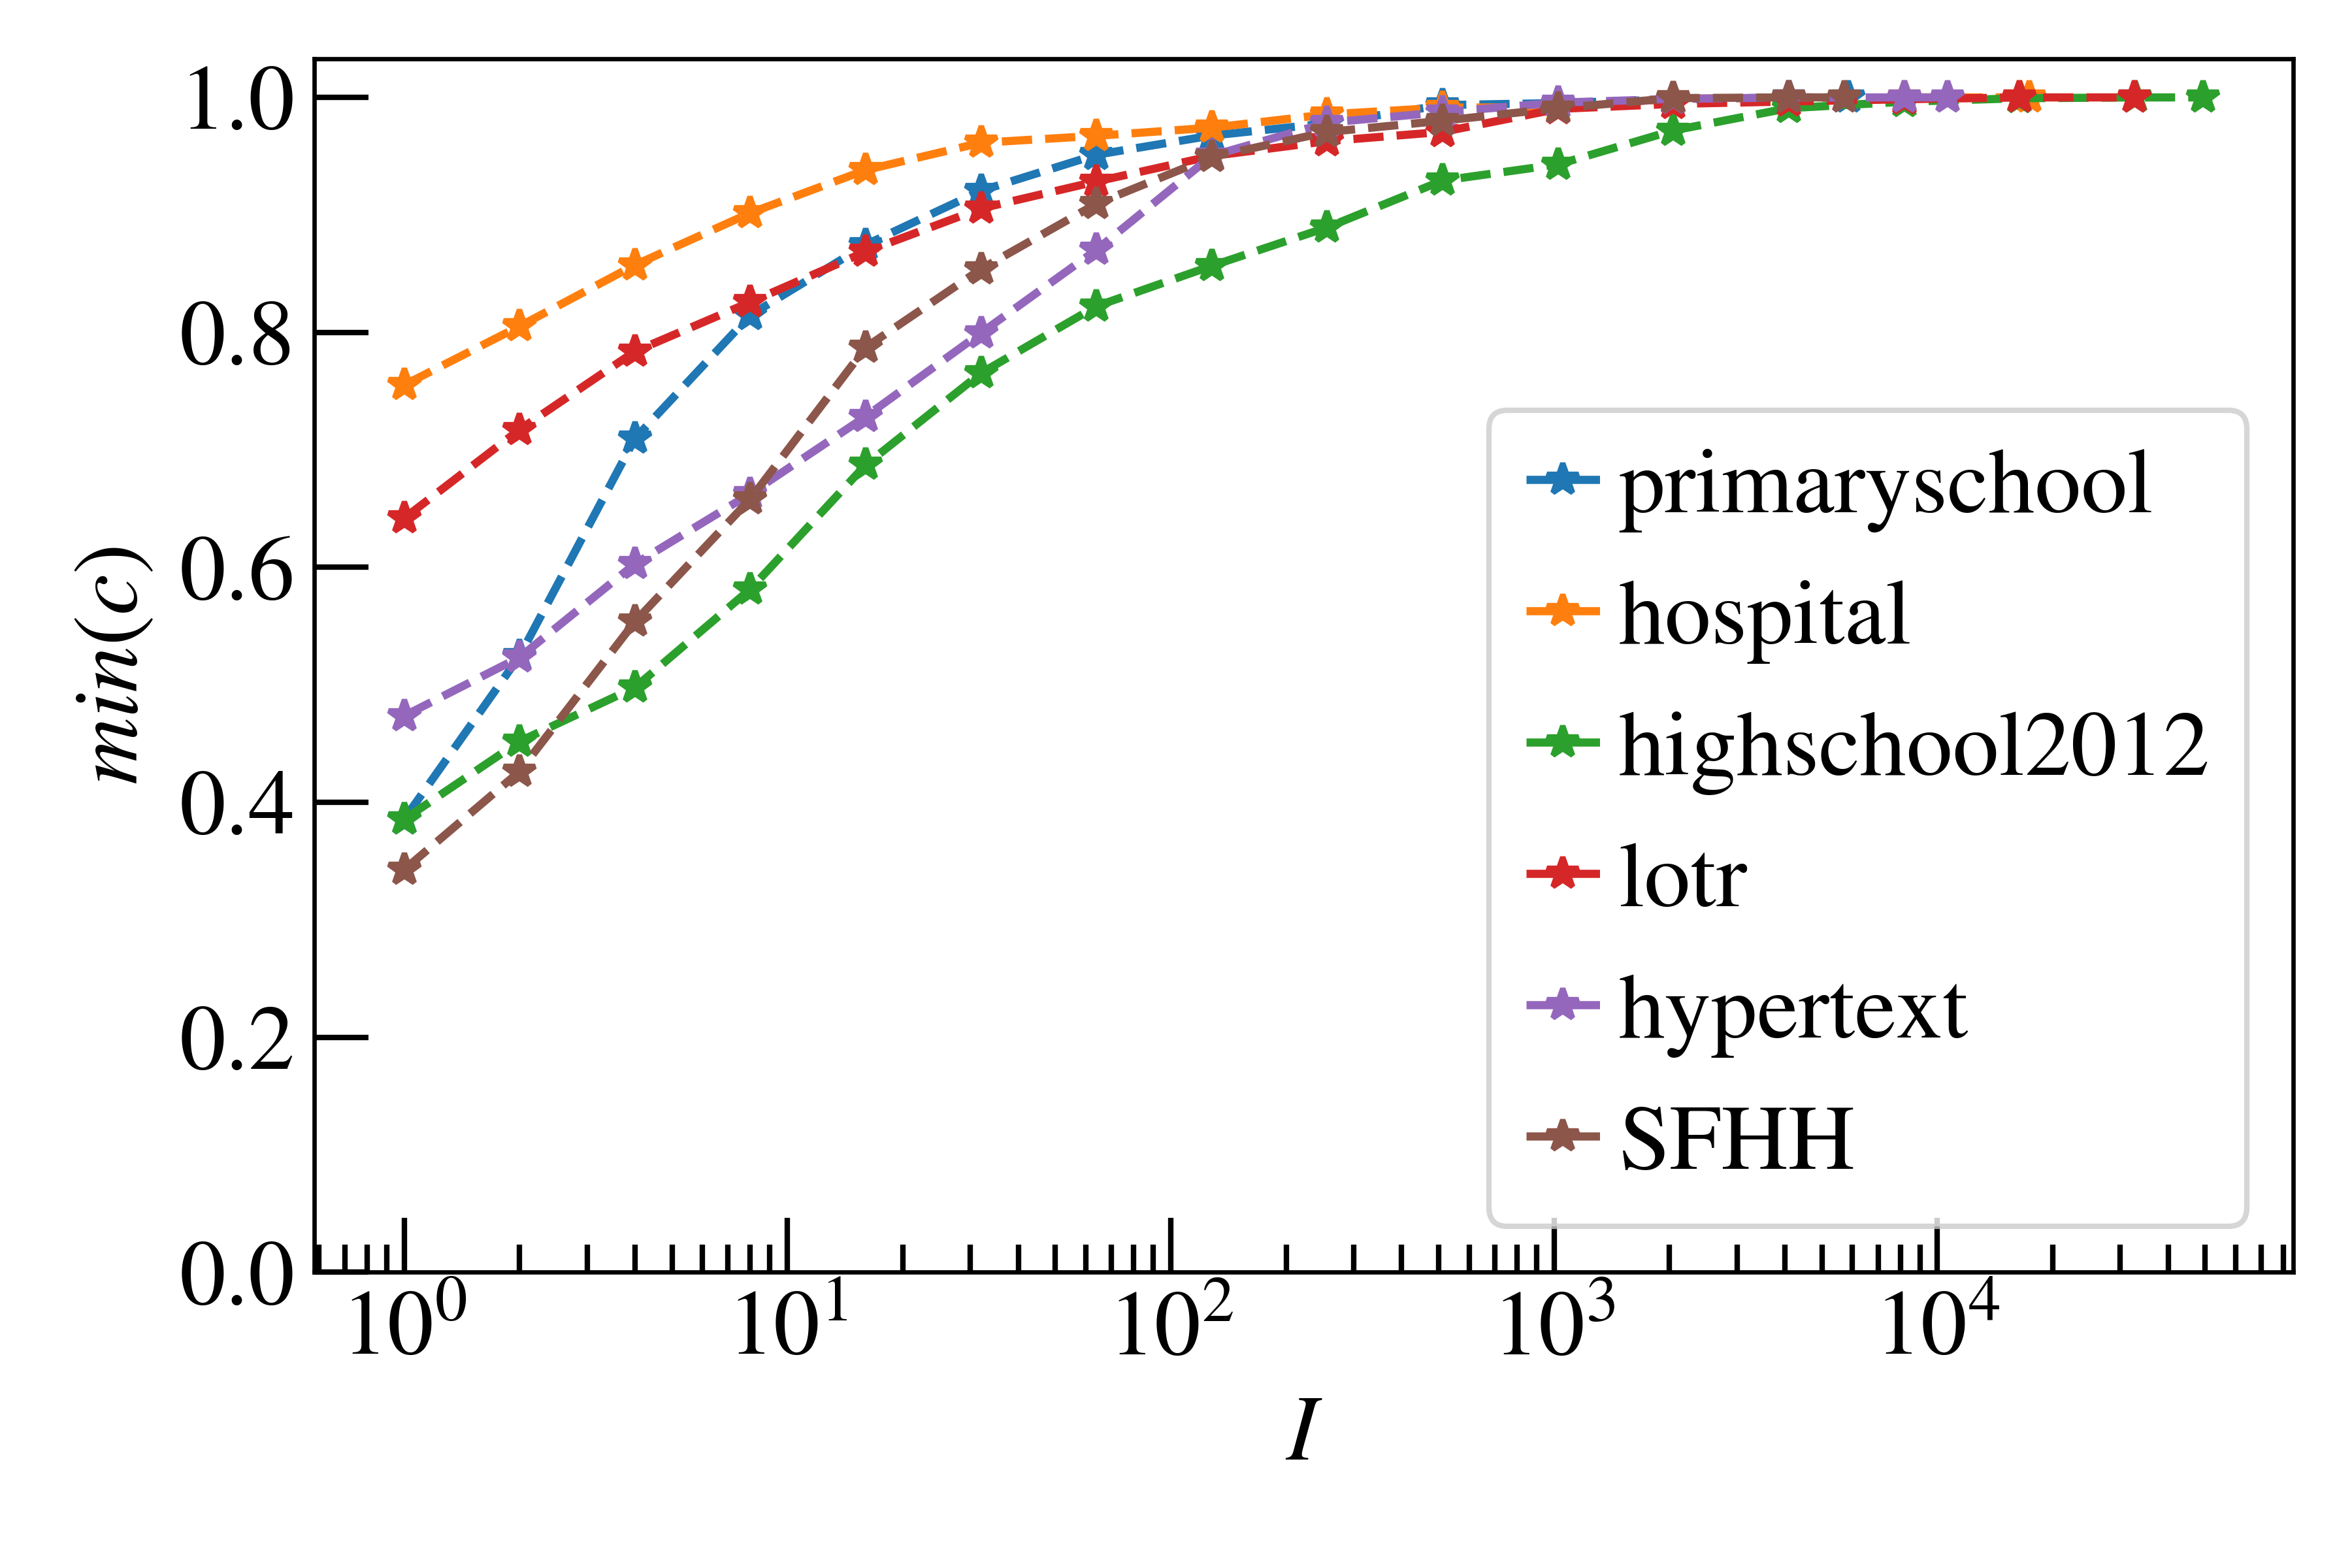
\includegraphics[width=0.48\textwidth]{fig/emp_min.png}
%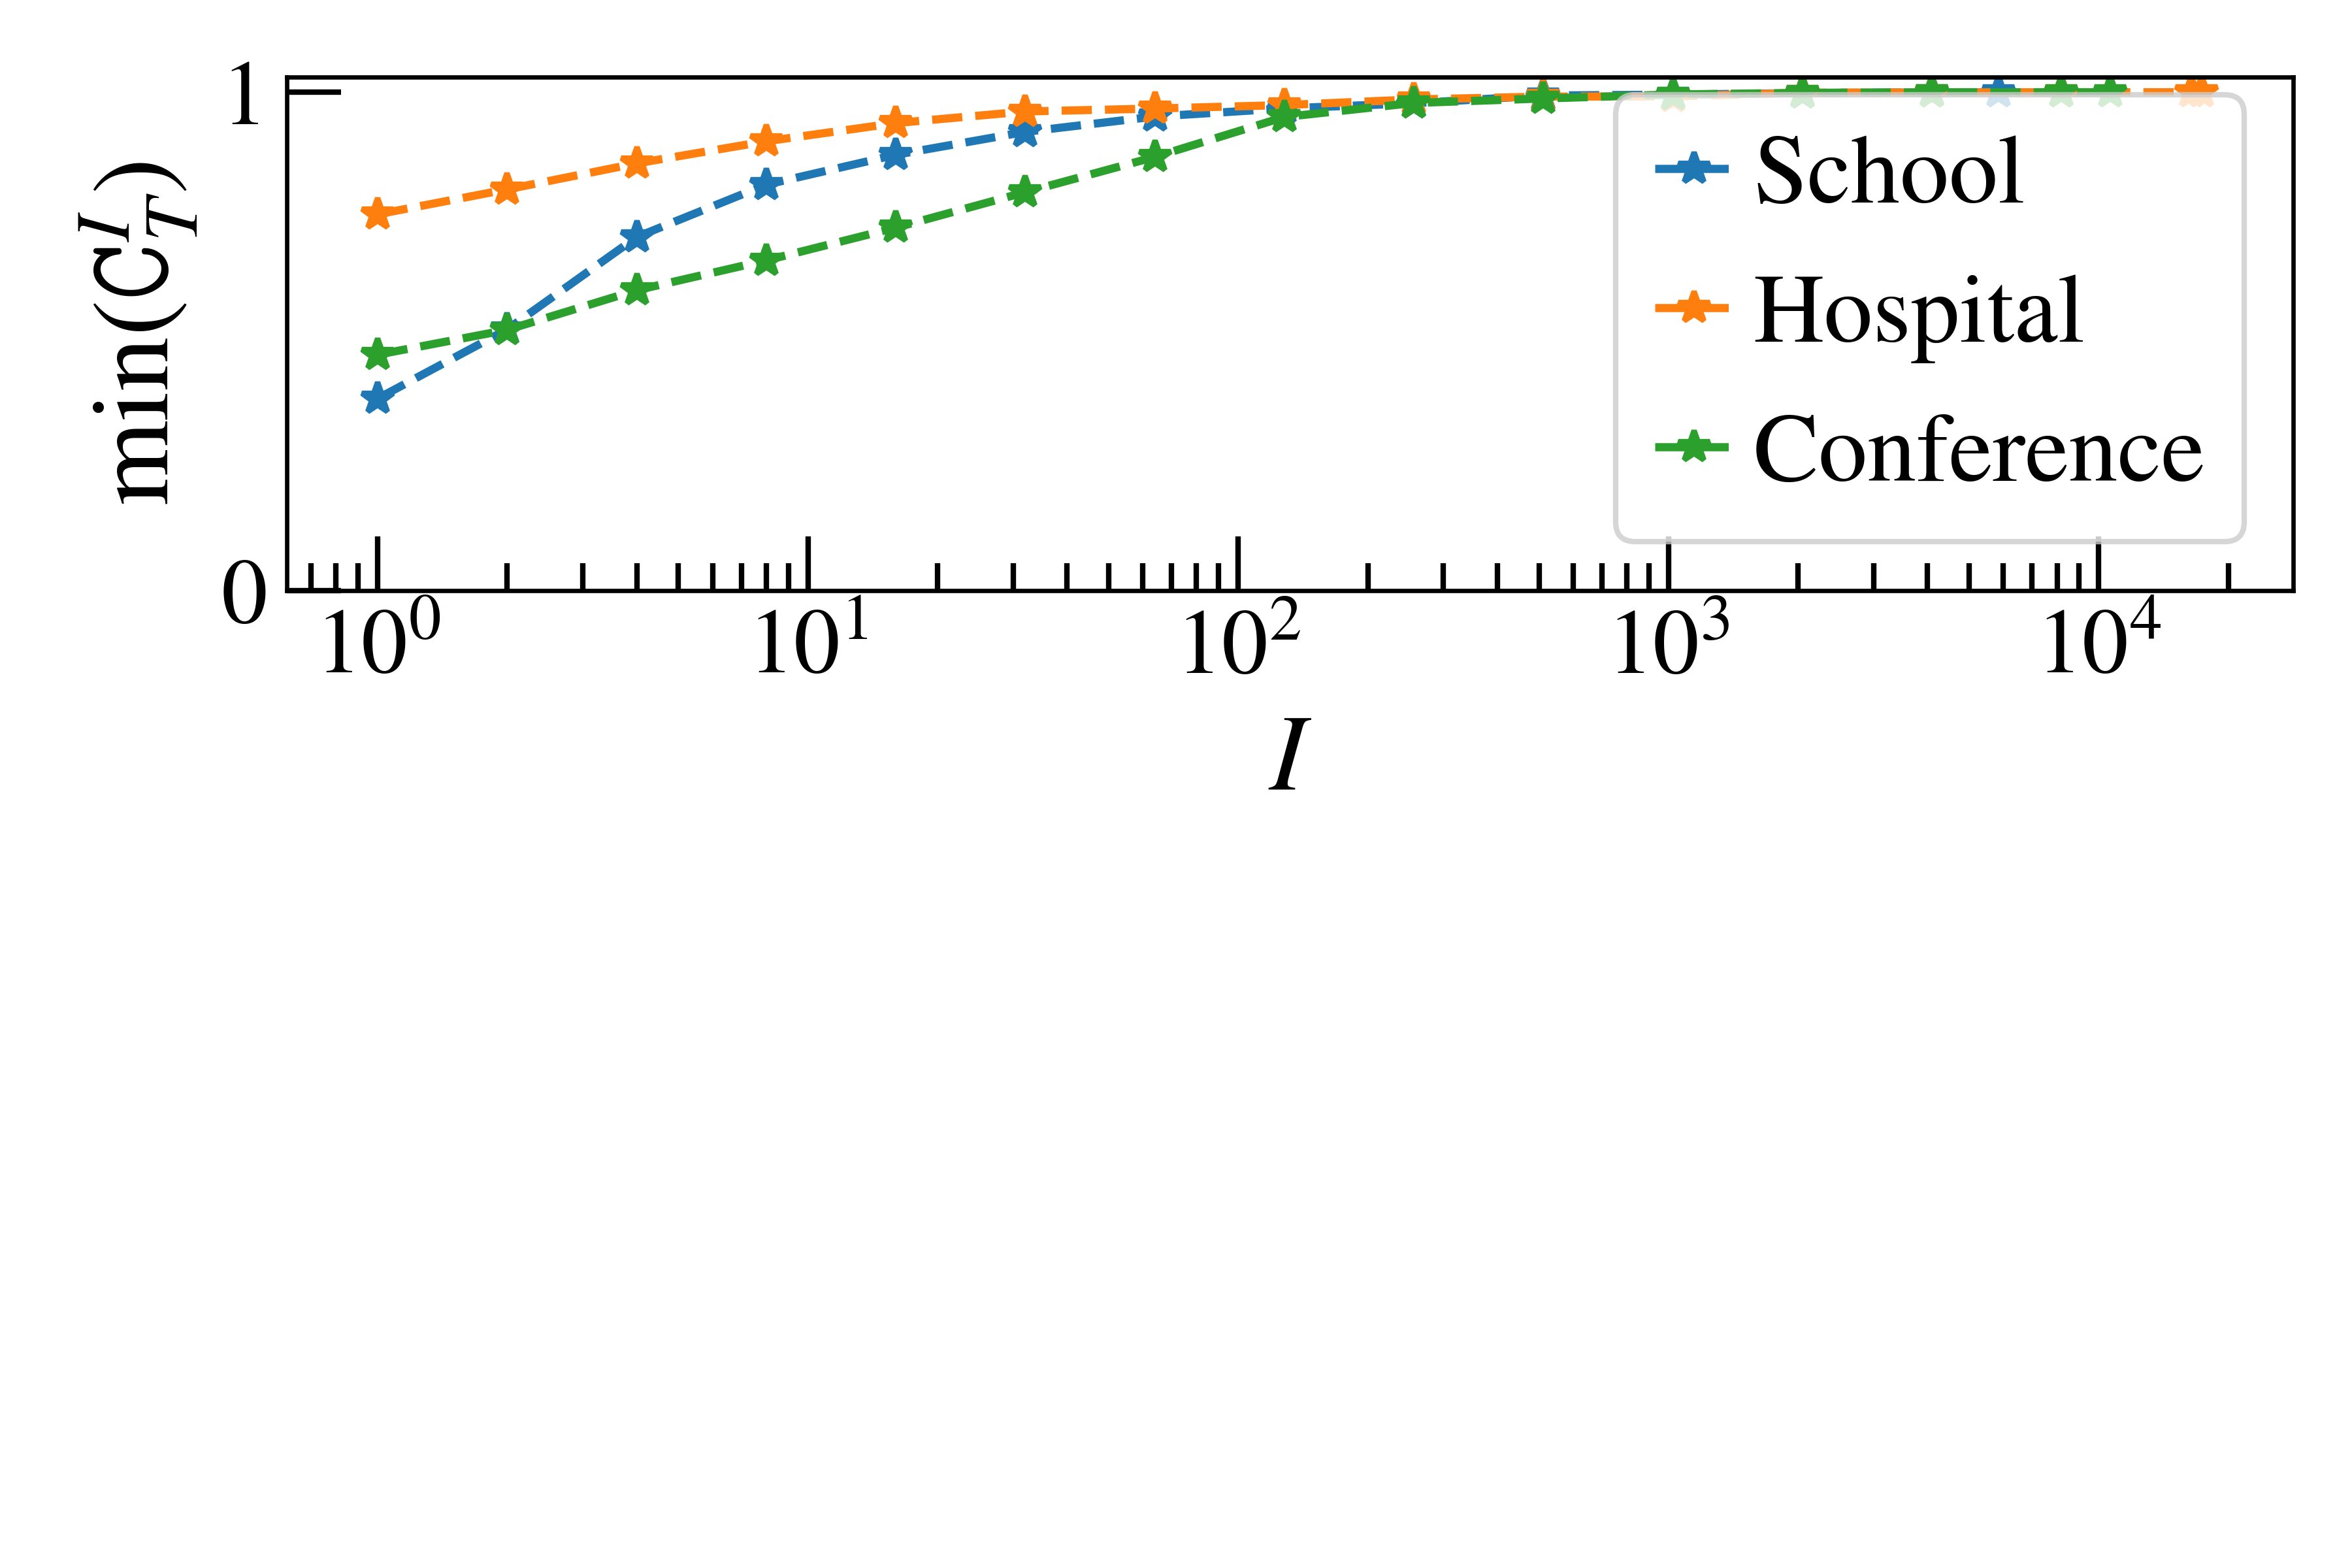
\includegraphics[width=0.48\textwidth]{fig/emp_ET_min_line.png}
\caption{\label{fig:dataMin}
Minima of the generalized causal fidelity as a function of the number of aggregation intervals $I$ for different datasets (upper panel) and their randomized versions (lower panel).
}
\end{figure}


\section{\label{sec:conclusions}Conclusions}
%what we did
In this paper we have addressed the problem of information loss for data aggregation in terms of the temporal accessibility graphs.
In particular, we have investigated how information loss regarding accessibility depends on the temporal network length and on the aggregation interval number.

To quantify how well an aggregated network represents the underlying original temporal network we have leveraged on the accessibility matrix to introduce a \emph{generalized causal fidelity} which measures how well an arbitrary temporal network represents a baseline temporal network. We have introduced sub-aggregated temporal networks that allow for arbitrary aggregation depth by slicing temporal networks into intervals of constant length.

The behavior of the generalized causal fidelity revealed the presence of an universal minimum for  both artificial and real networks. We characterize this minimum, which identifies the maximum information loss range, in terms of the underlying fully  aggregated network and in particular by the emergence of giant components and their saturation as temporal network length is increased.

By considering uncorrelated temporal snapshots we get insights into characteristics of temporal networks that drive the generalized causal fidelity. For the case of full aggregation, i.e. when aggregating the whole temporal network into one snapshot,  we presented a simple model that related the expected density of the accessibility of the fully aggregated network to the edge probability of each snapshot and the total number of snapshots of the random temporal networks.  
By inverting this relation we obtained a functional dependence of temporal network length and the density of both individual snapshots and aggregated representation. The values of the temporal network length that corresponds to the critical point for percolation in the aggregated network and to the giant component saturation define the interval in temporal network lengths where the aggregate representation of a given temporal network is least appropriate, as information loss due to aggregation is then maximal. 
This analytical approach gives the insight that the generalized causal fidelity is mainly driven by emerging connectedness in the aggregated network that is not present in the non-aggregated contribution of the temporal accessibility. 
% Since in the aggregated temporal network the connectedness, and thereby accessibility, emerges faster then in the temporal network, the generalized causal fidelity shows a valley pattern in the range where connectedness emerged in the aggregated network, but lags behind in the non-aggregated network. 
% %SBM
We showed that, when random temporal networks with distinct temporal communities are considered, connectedness can emerge at different stages of temporal network lengths.
%SF
For arbitrary degree sequences we showed how the presence of highly connected nodes results in minimal information loss.

The analysis of sub-aggregated temporal networks reveals that with few aggregation intervals, the expected worst case can be improved substantially compared to only one aggregation interval.  
However, the marginal effect of considering additional aggregation intervals rapidly decreases.
%EMP
For all analyzed datasets,  
we correctly estimated the location of the valley of the generalized causal fidelity where aggregation yields maximal information loss.  
\fla{comment on dataset degree heterogeneity}
% For all analyzed datasets we provided a simple analytical expression for the saturation value $T_f$ such that for $T>T_f$ information loss is always negligible compared to the worse case scenario for any aggregated representation and depending only on the number of nodes and on the average snapshot density.
%critical comments
Importantly, empirical temporal networks presents a combination of different  effects that are not present in simple random temporal networks, such as community structure, different activity rates, and many others. 
Despite this, the insights from random temporal network give an intuition into some of the relevant processes that may characterize information loss in real systems.  These insights and the analytical results rely on the independence between the snapshots and edges. 
% In general, these insights are mainly insightful for ongoing, stationary process. E.g. if a temporal network is considered where nodes join over time, and others drop out and ore not active anymore, it is not clear how the behavior looks like, since in these cases the original temporal network does not have the chance to close path to nodes that are not active anymore.
It remains a challenge for futures works to generalize this approach to correlated temporal snapshots and to include important temporal network features such as edge burstiness.


\vspace{0.5cm}
\begin{acknowledgments}
 FI acknowledges funding of SNSF (Switzerland) through project  200021\_182659. CJT acknowledges financial support from the  University of Zurich through the University Research Priority Program on Social Networks. 
\end{acknowledgments}

%\appendix


\bibliography{biblio,apssamp}
\end{document}